\documentclass[11pt]{article}

\usepackage[margin=1in]{geometry}
\usepackage{setspace}
\onehalfspacing
\usepackage{graphicx}
\graphicspath{report_images/}
\usepackage{appendix}
\usepackage{listings}
\usepackage{float}
\usepackage{multirow}
\usepackage{amsthm}
% The next three lines make the table and figure numbers also include section number
\usepackage{chngcntr}
\counterwithin{table}{section}
\counterwithin{figure}{section}
% Needed to make titling page without a page number
\usepackage{titling}

% DOCUMENT INFORMATION =================================================
\font\titleFont=cmr12 at 11pt
\title {{\titleFont ECEN 429: Introduction to Digital Systems Design Laboratory \\ North Carolina Agricultural and Technical State University \\ Department of Electrical and Computer Engineering}} % Declare Title
\author{\titleFont Reporter: Nikiyah Beulah \\ \titleFont Partner: Chris Cannon} % Declare authors
\date{\titleFont March 29, 2018}
% ======================================================================

\begin{document}

\begin{titlingpage}
\maketitle
\begin{center}
	Lab 8
\end{center}
\end{titlingpage}

\section{Introduction}
This lab tested our ability to implement a counter and control that counter by implementing a finite state machine. These tasks represent basic digital design skills where we are given a real task to implement and utilizing an integrated finite state machine to control it.

\section{Background, Design Solution, and Results}

\subsection{Problem 1 }

\subsubsection{Background}
Problem 1 requires a simple counter that can count up and down, with no other features required. This basic counter is simple to implement, it requires only an integer getting iterated up or down.

\subsubsection{Design Solution}
We used the clock divider developed in Lab 6 to help make this unit testable. We displayed our current count on a seven-segment display. We used a temporary count signal that will count up or down and then will be translated to the seven-segment display. The input ports are summarized in Table ~\ref{tab:counter_input_Ports} and the output ports are summarized in Table ~\ref{tab:counter_output_Ports}.

\begin{table}[H]
\begin{center}
\begin{tabular}{| l | l | l |}
	\hline
	Bit & Label & Port \\ \hline
	clk & Clock & W5 \\ \hline
	direction & Switch 0 & V17 \\ \hline
	reset & Button R & T17 \\ \hline
\end{tabular}
\caption{\label{tab:counter_input_Ports}Input port assignments for  the counter.}
\end{center}
\end{table}

\begin{table}[H]
\begin{center}
\begin{tabular}{| l | l | l |}
	\hline
	Bit & Label & Port \\ \hline
	clk led & LED 15 & L1 \\ \hline
	count6 & CA & W7 \\ \hline
	count5 & CB & W6 \\ \hline
	count4 & CC & U8 \\ \hline
	count3 & CD & V8 \\ \hline
	count2 & CE & U5 \\ \hline
	count1 & CF & V5 \\ \hline
	count0 & CG & U7 \\ \hline
\end{tabular}
\caption{\label{tab:counter_output_Ports}Output port assignments for counter.}
\end{center}
\end{table}

\subsubsection{Results}
The counter worked as expected and selected results are shown in Figures ~\ref{fig:counter_res1} through ~\ref{fig:counter_res6}.

\begin{figure}[H]
\begin{center}
	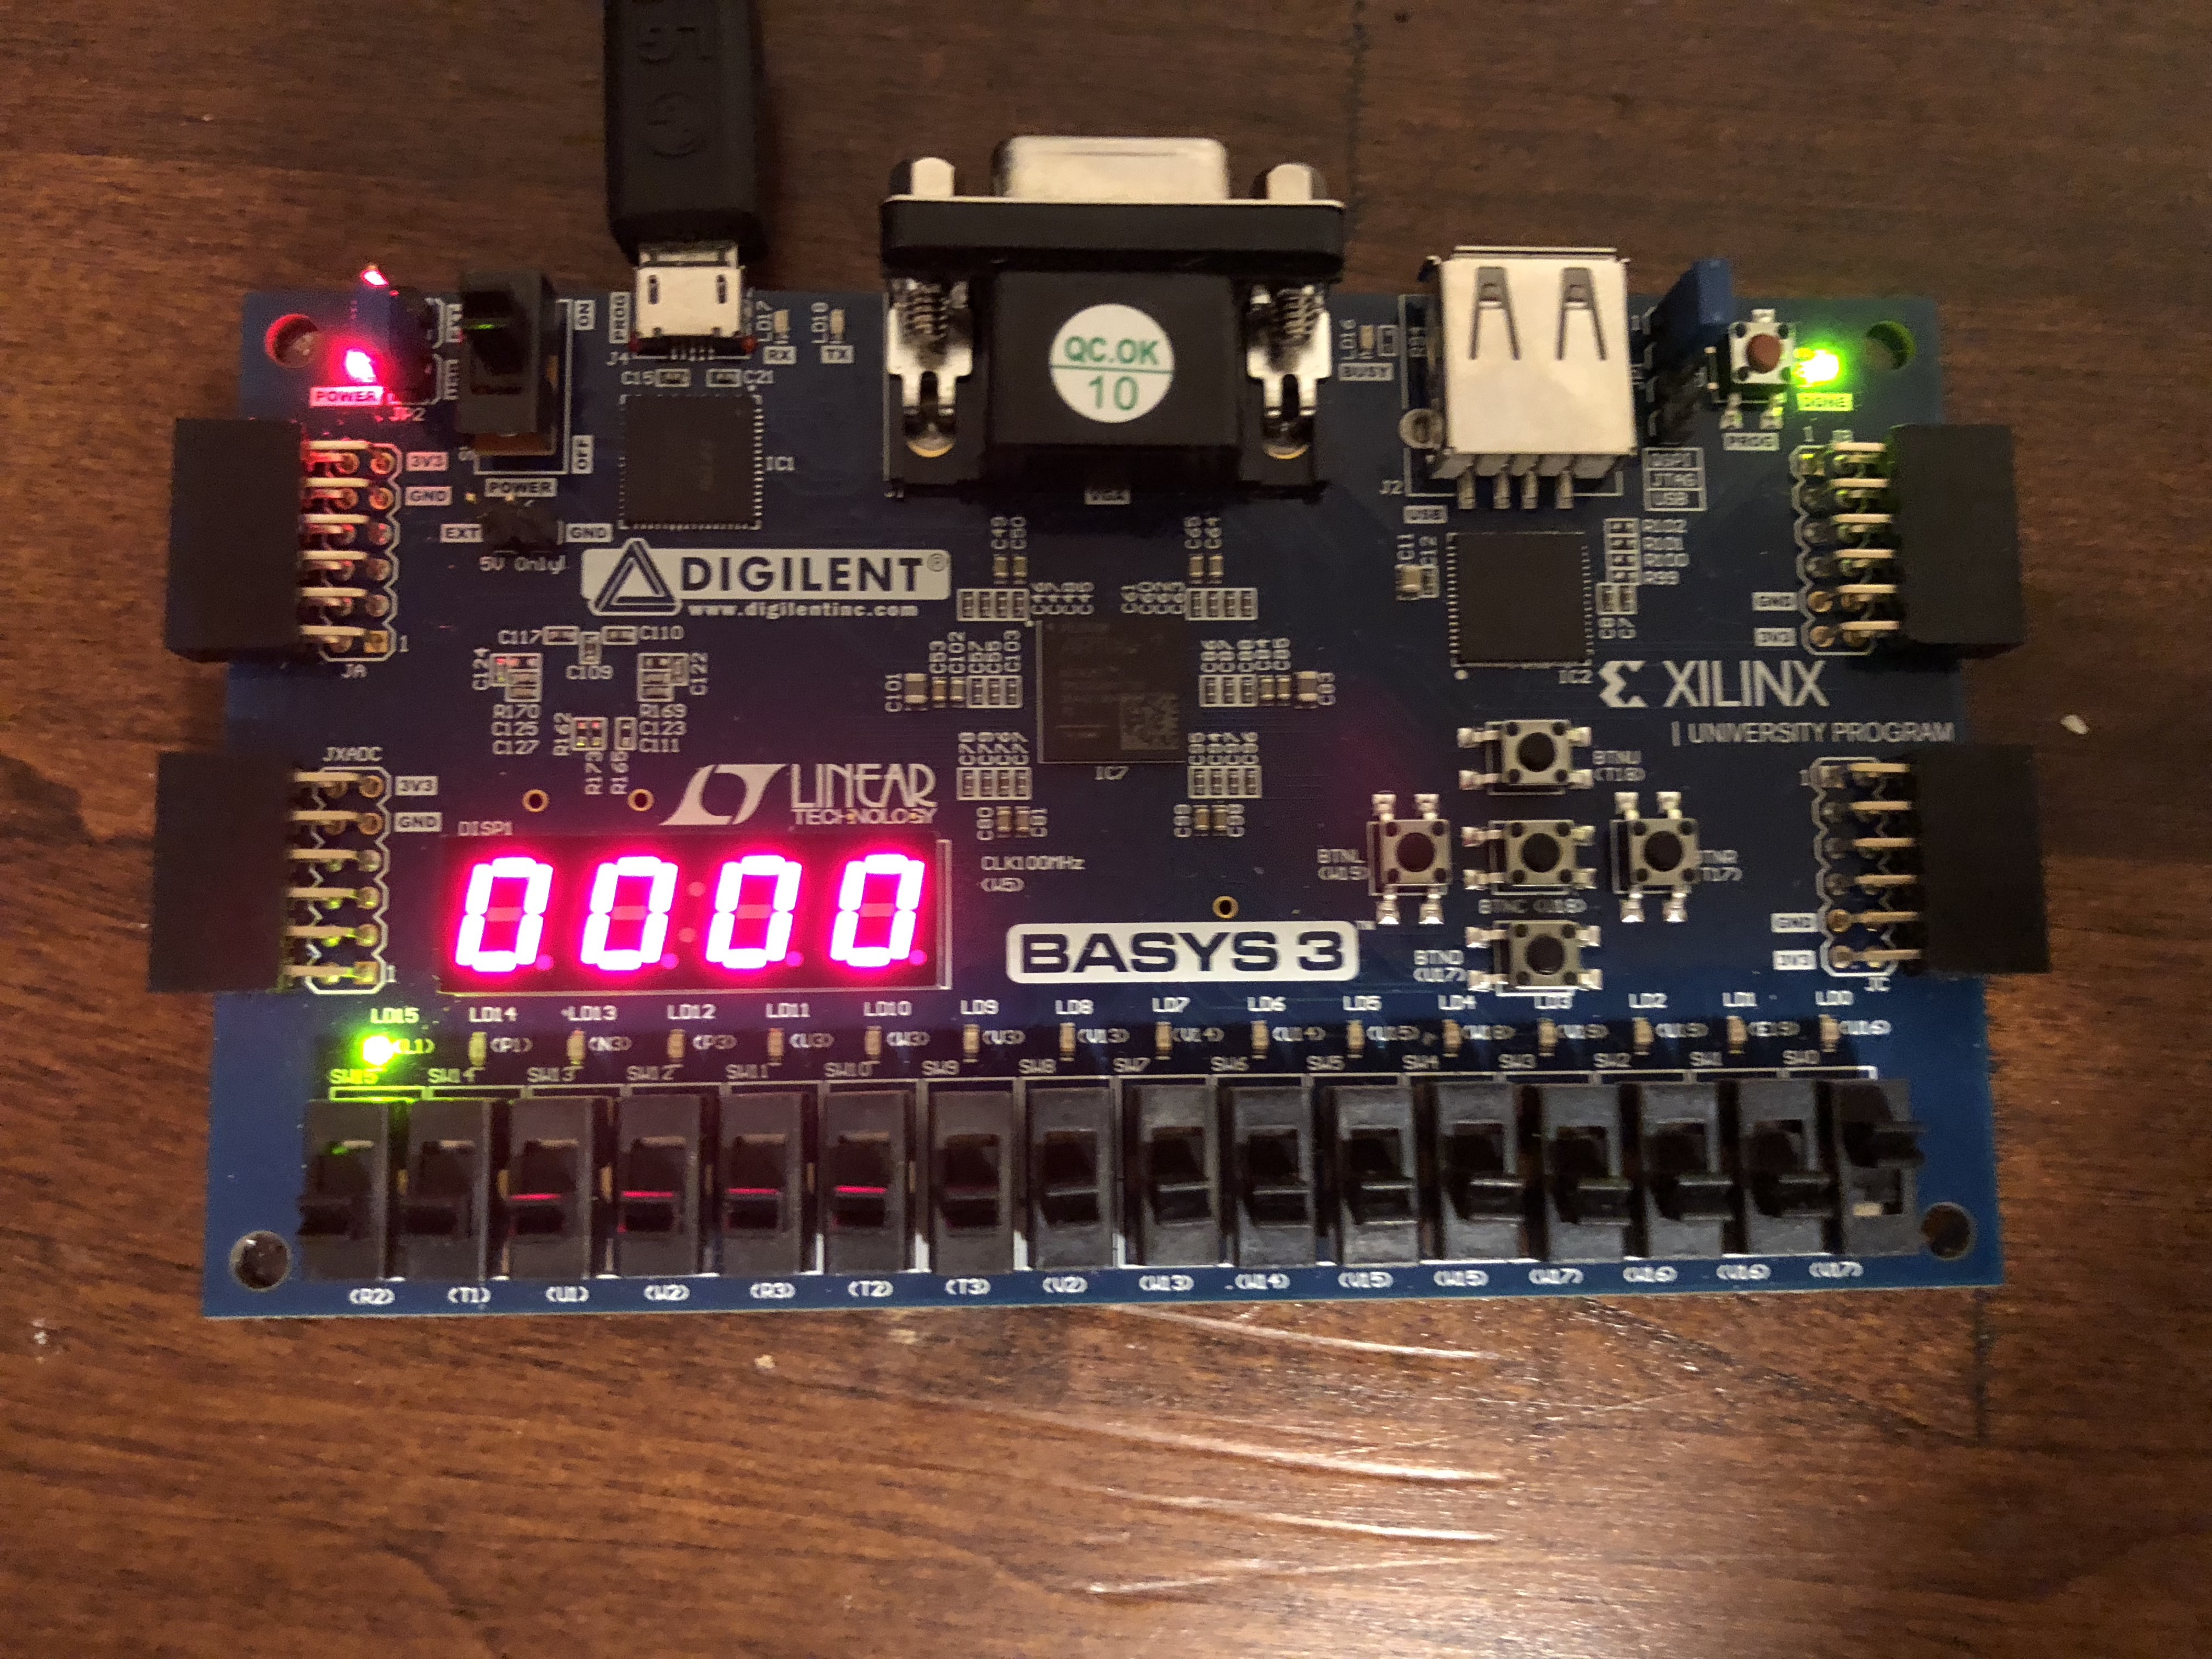
\includegraphics[width=0.5\textwidth]{./images/p1/IMG_1001.jpg}
	\caption{\label{fig:counter_res1}Counting up, at 0. Direction Switch 1 is on.}
\end{center}
\end{figure}

\begin{figure}[H]
\begin{center}
	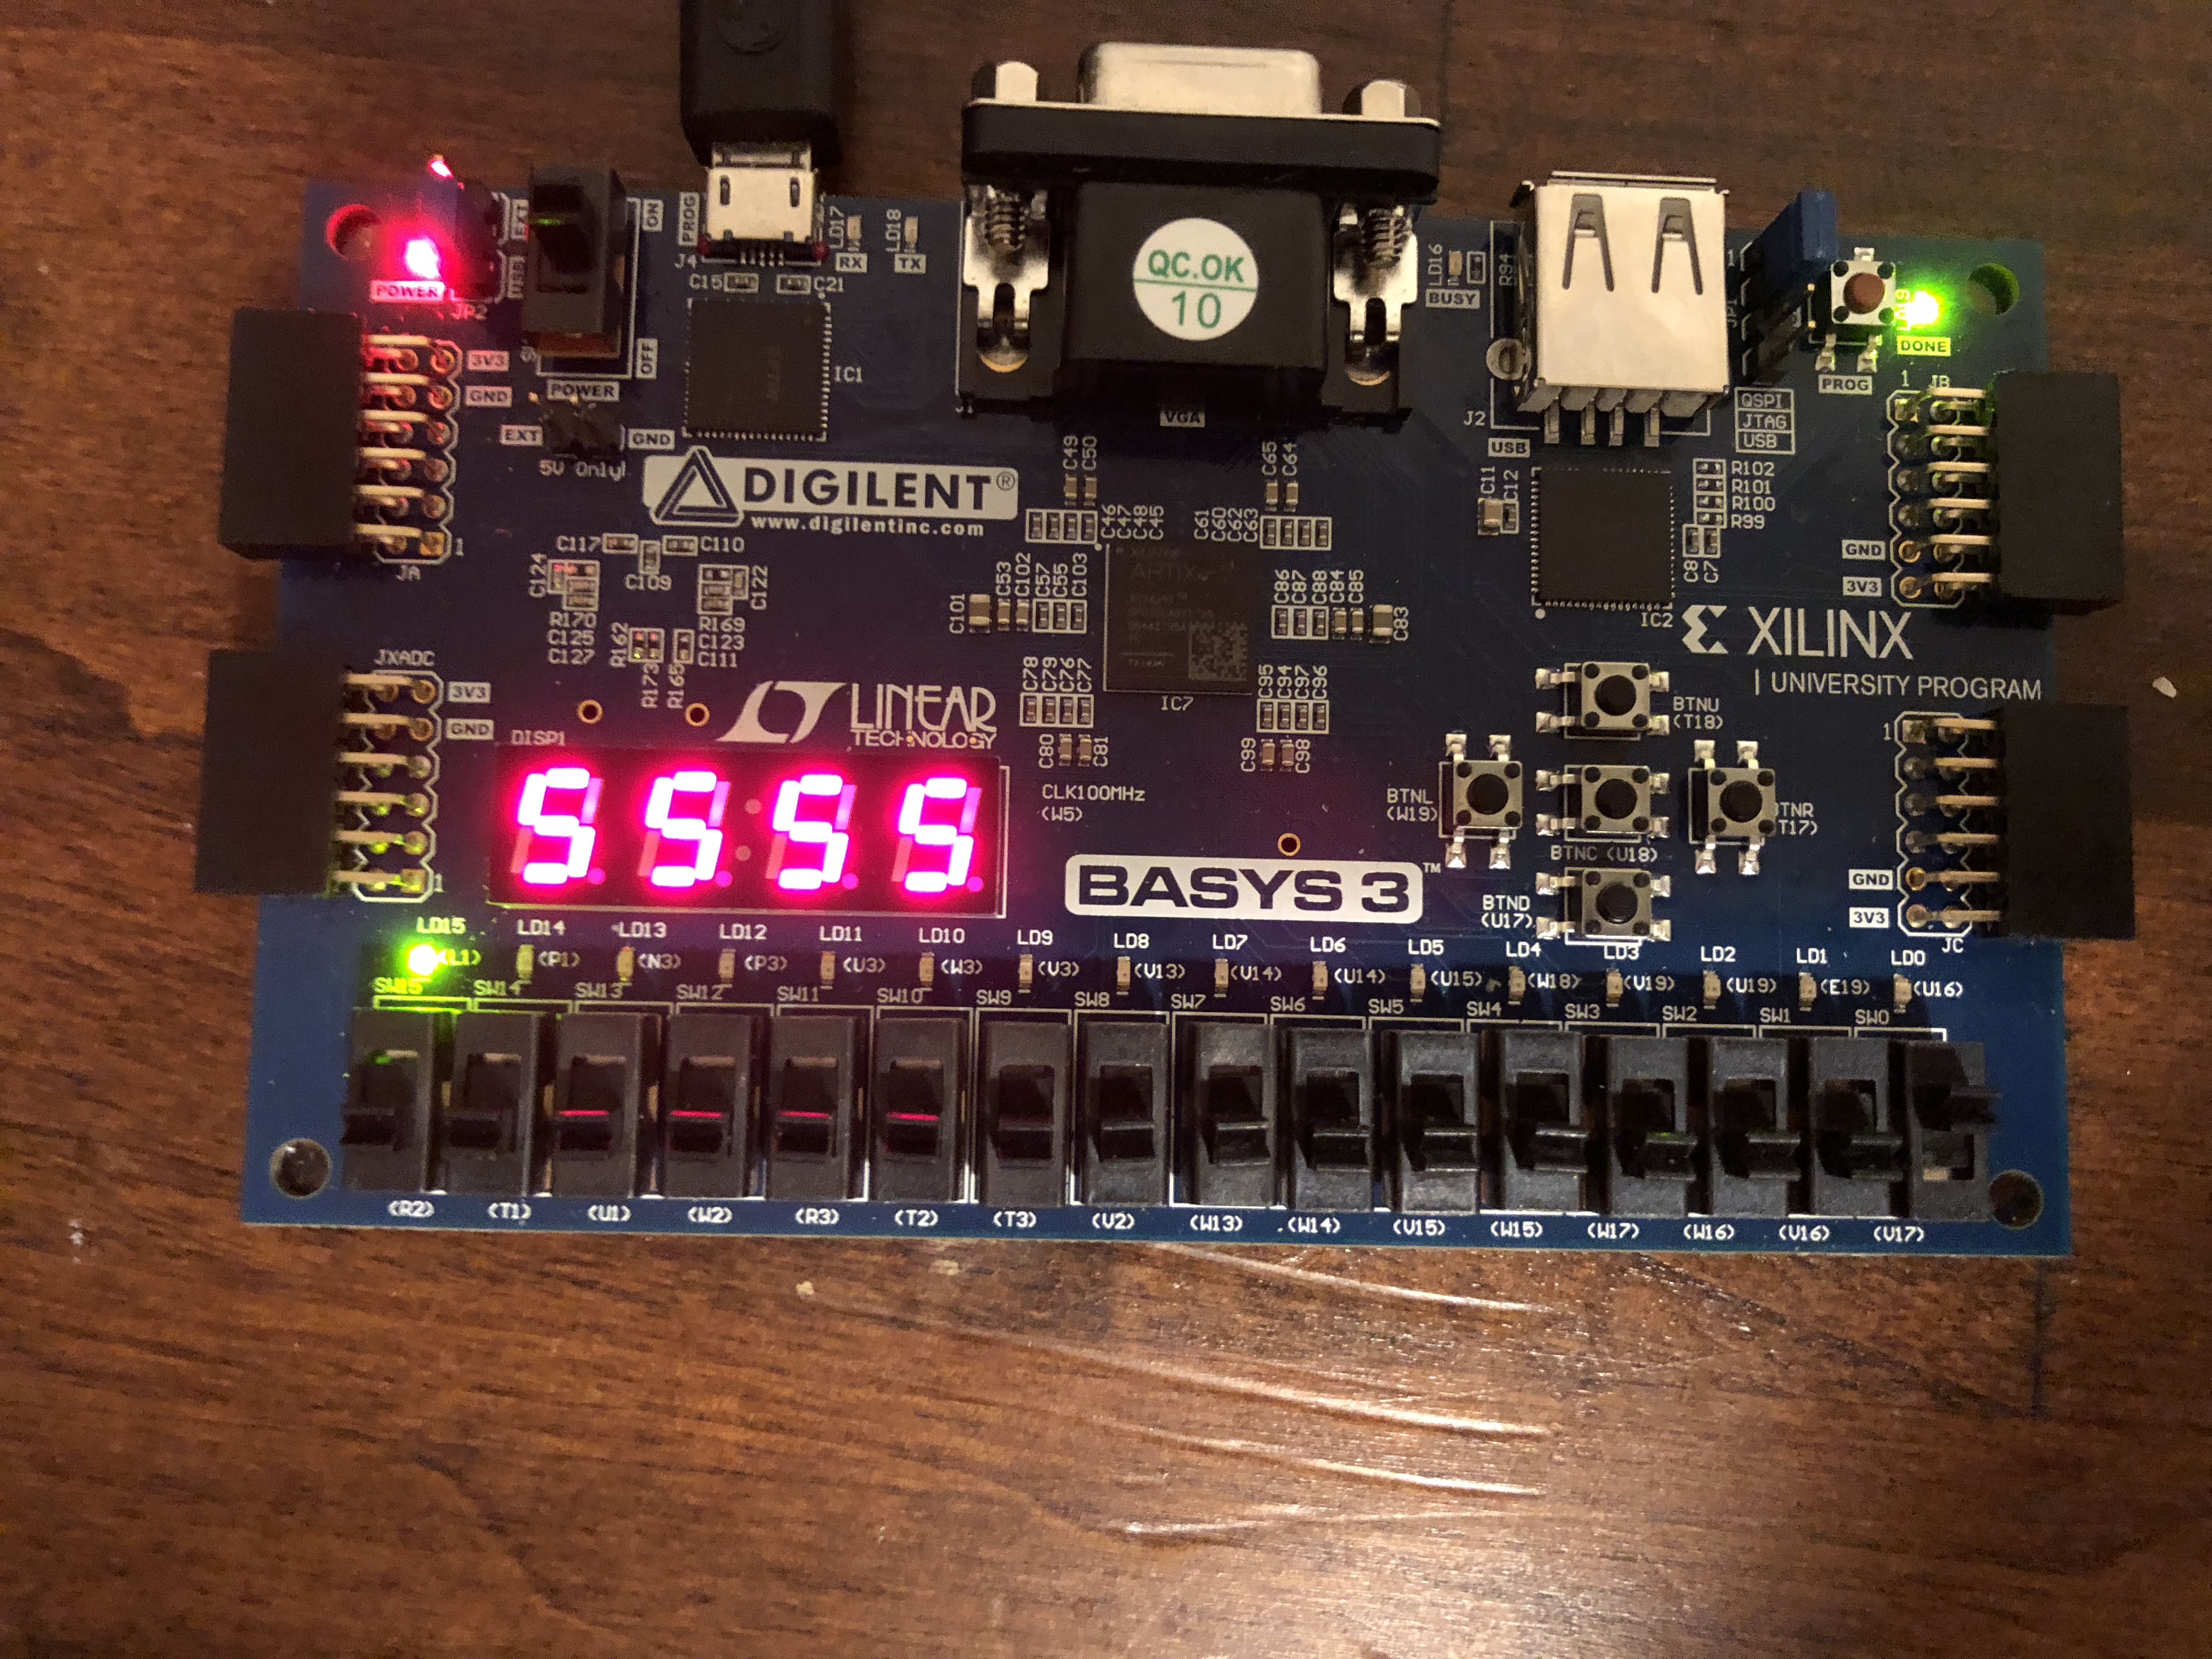
\includegraphics[width=0.5\textwidth]{./images/p1/IMG_1002.jpg}
	\caption{\label{fig:counter_res2}Counting up, at 5. Direction Switch 1 is on.}
\end{center}
\end{figure}

\begin{figure}[H]
\begin{center}
	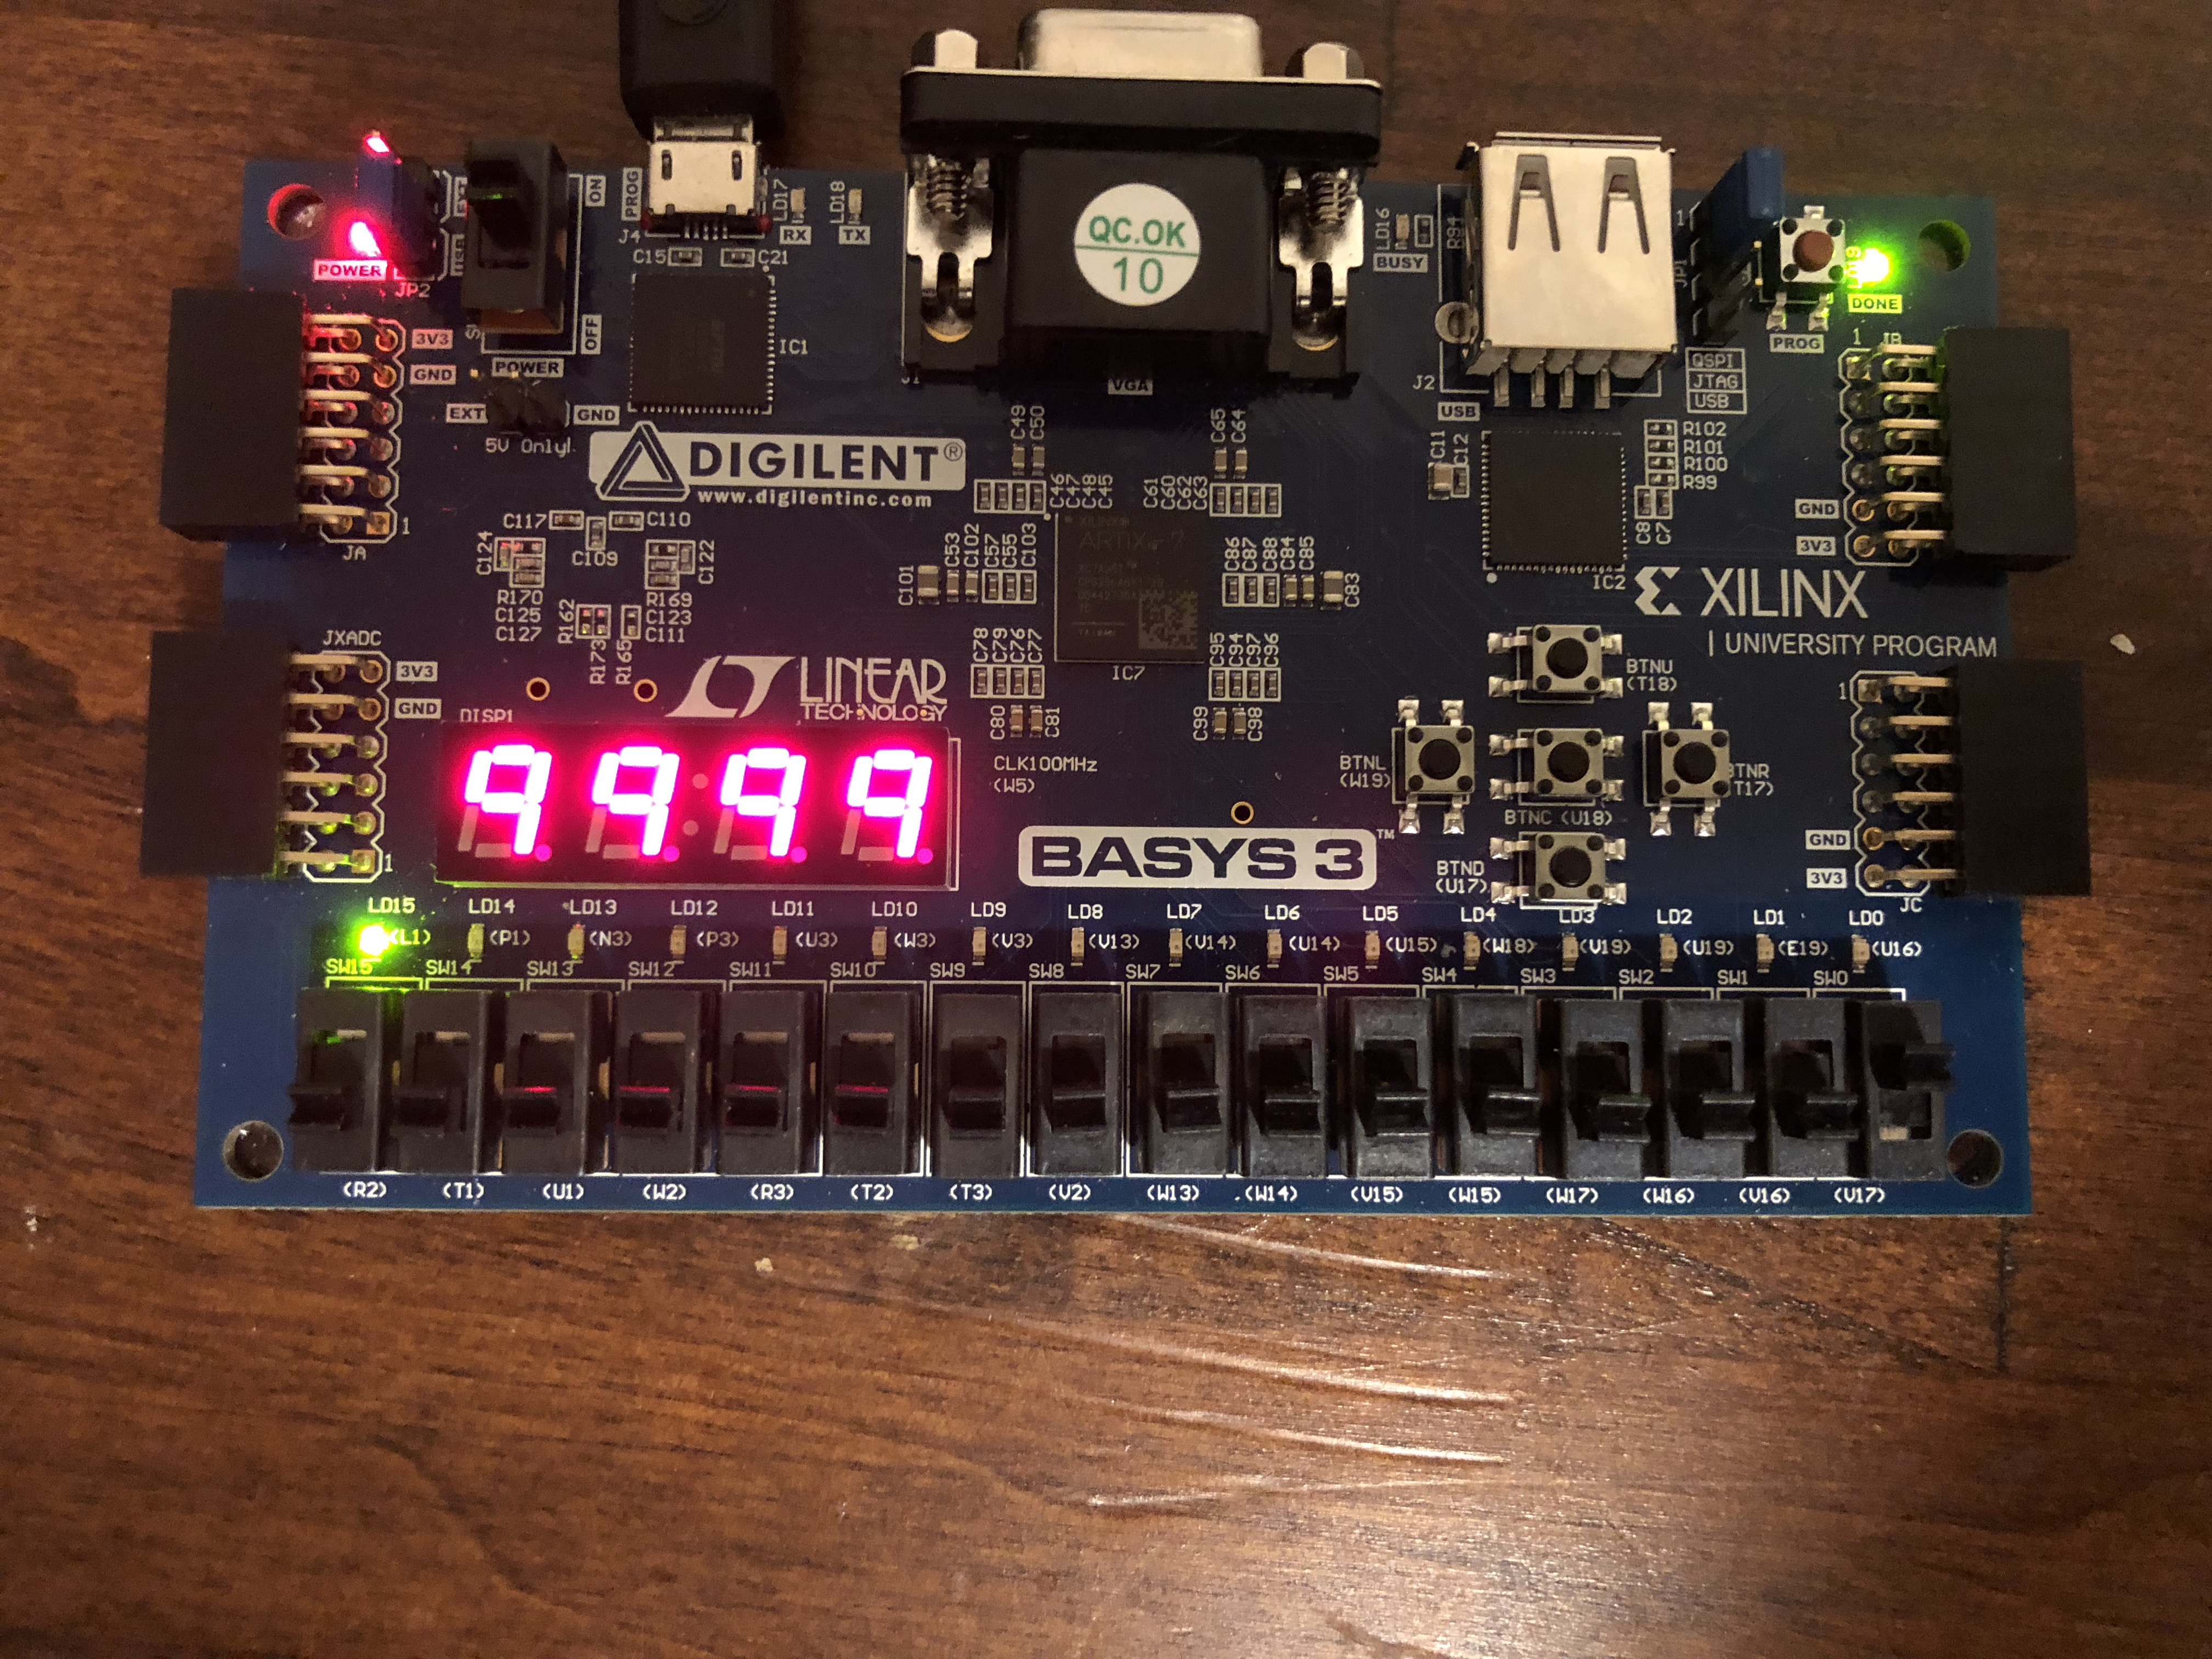
\includegraphics[width=0.5\textwidth]{./images/p1/IMG_1003.jpg}
	\caption{\label{fig:counter_res3}Counting up, at 9. Direction Switch 1 is on.}
\end{center}
\end{figure}

\begin{figure}[H]
\begin{center}
	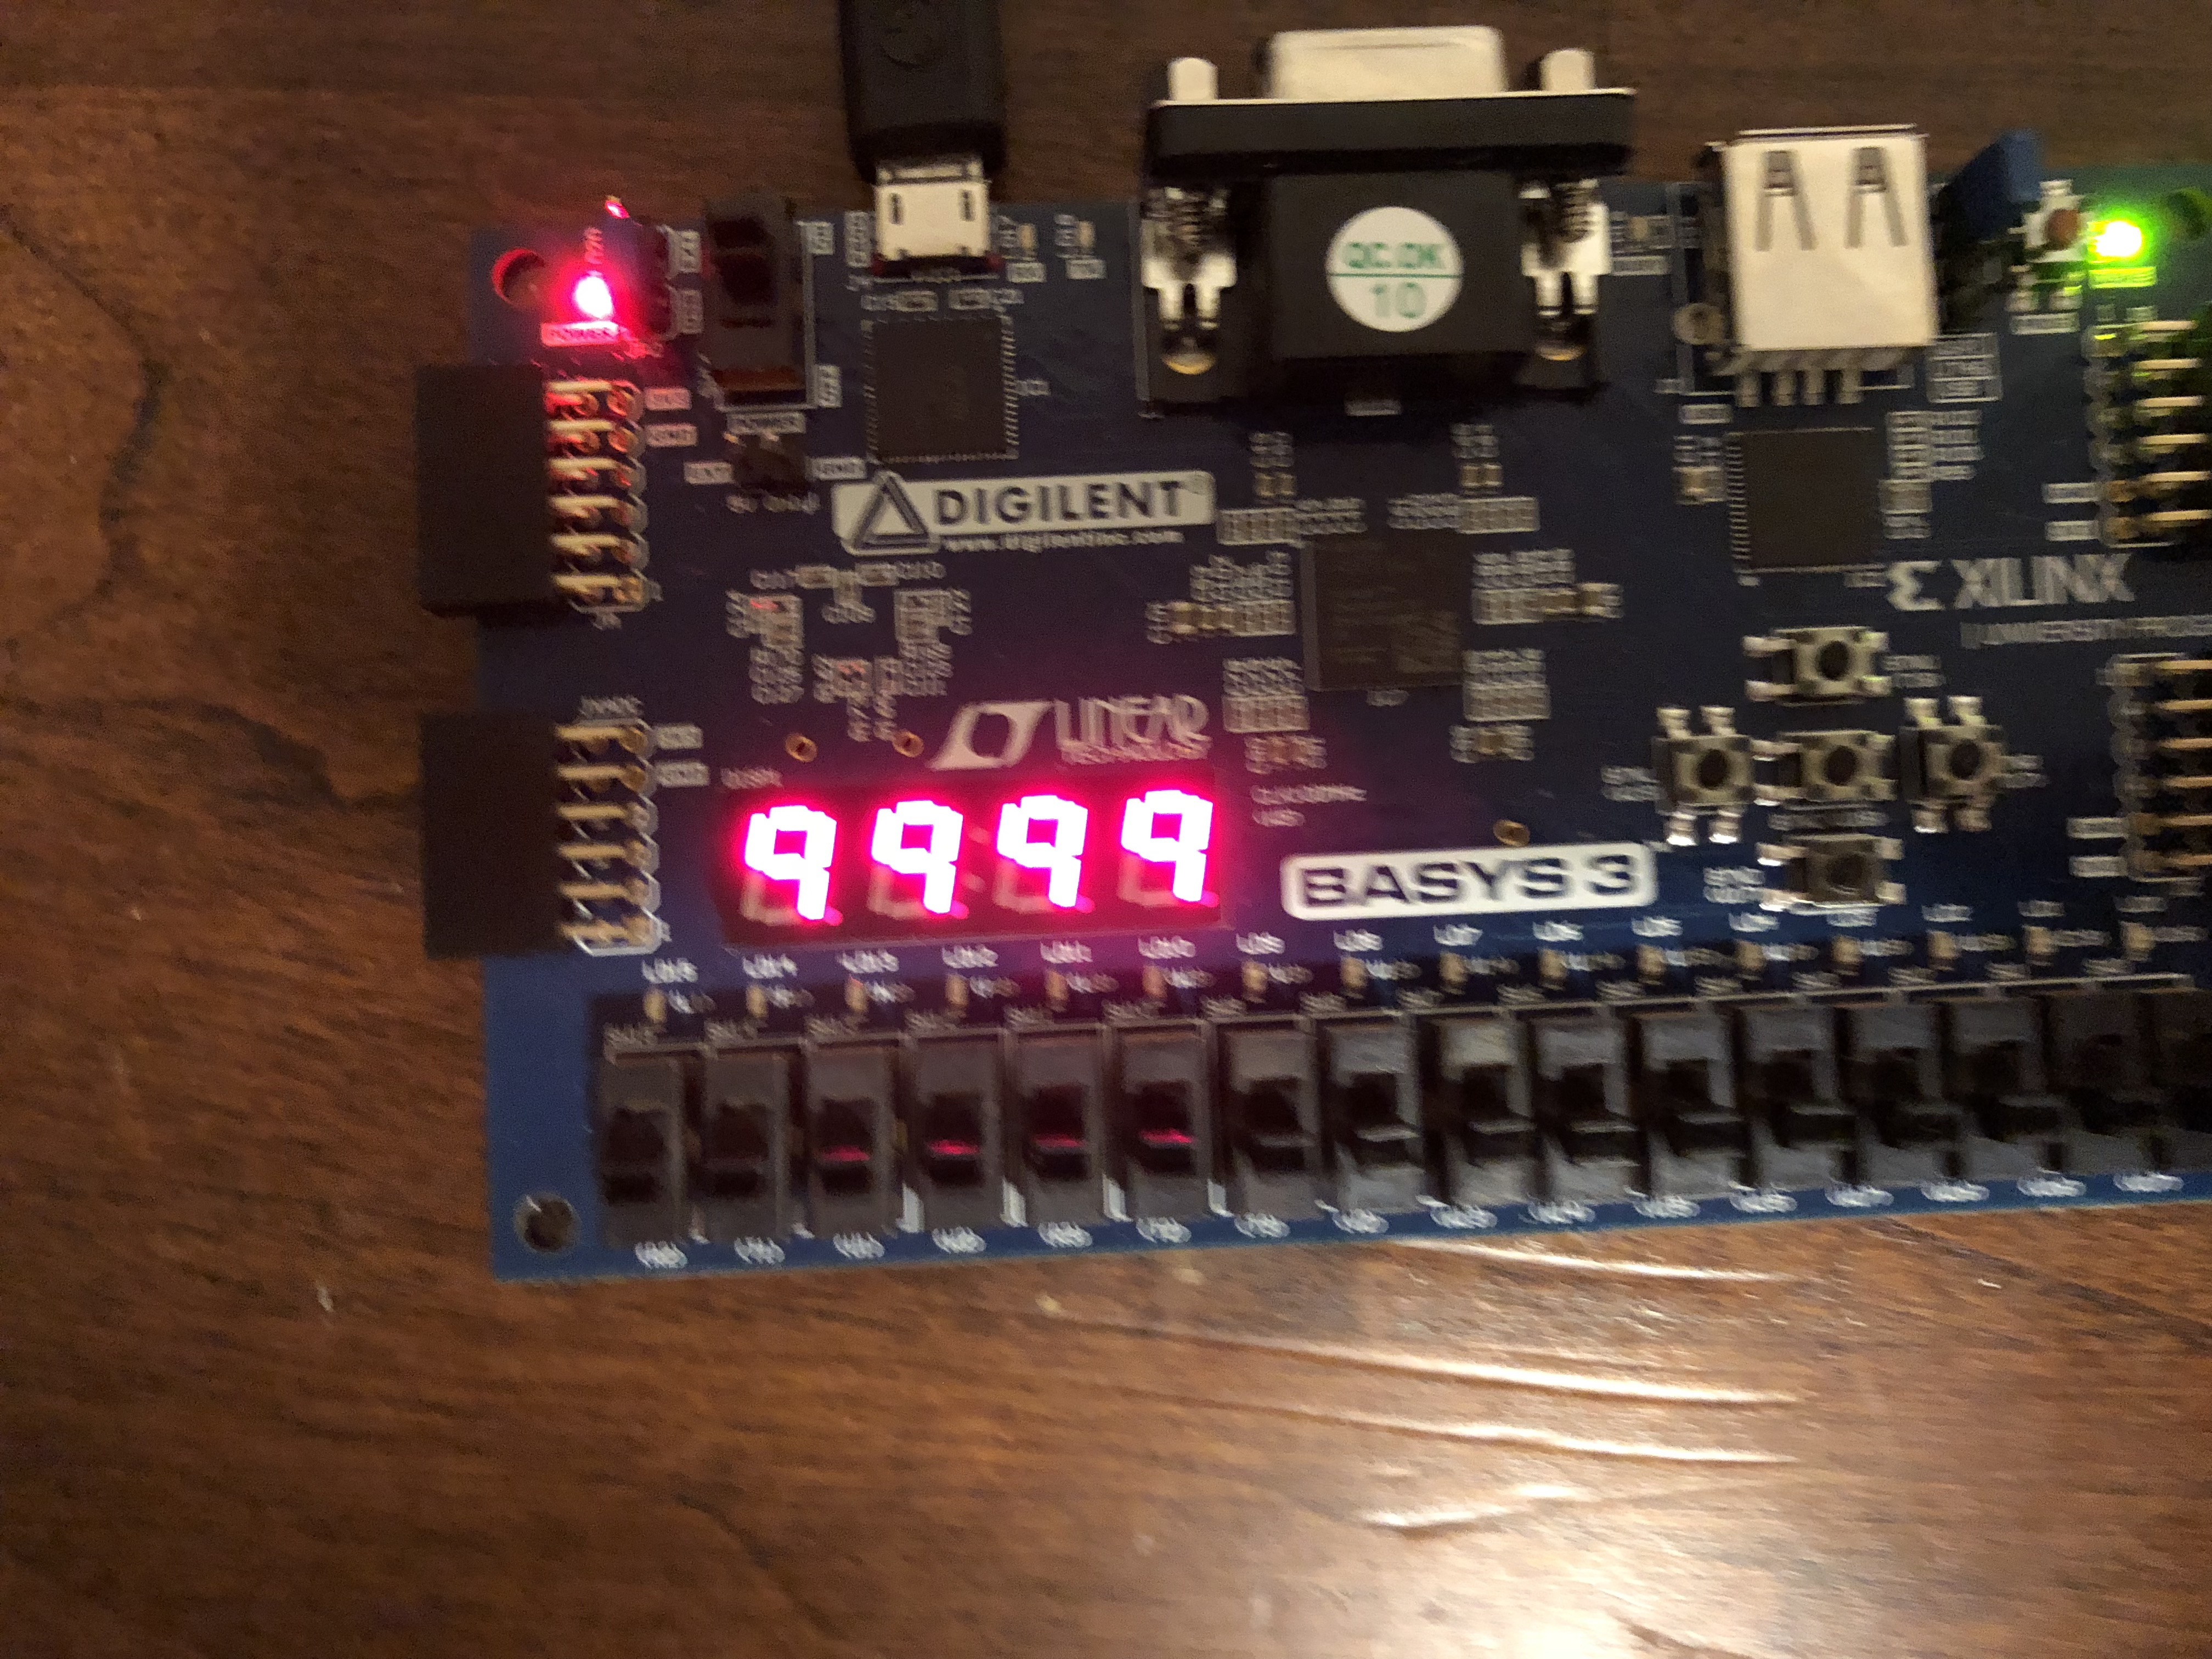
\includegraphics[width=0.5\textwidth]{./images/p1/IMG_1004.jpg}
	\caption{\label{fig:counter_res4}Counting down, at 9. Direction Switch 1 if off.}
\end{center}
\end{figure}

\begin{figure}[H]
\begin{center}
	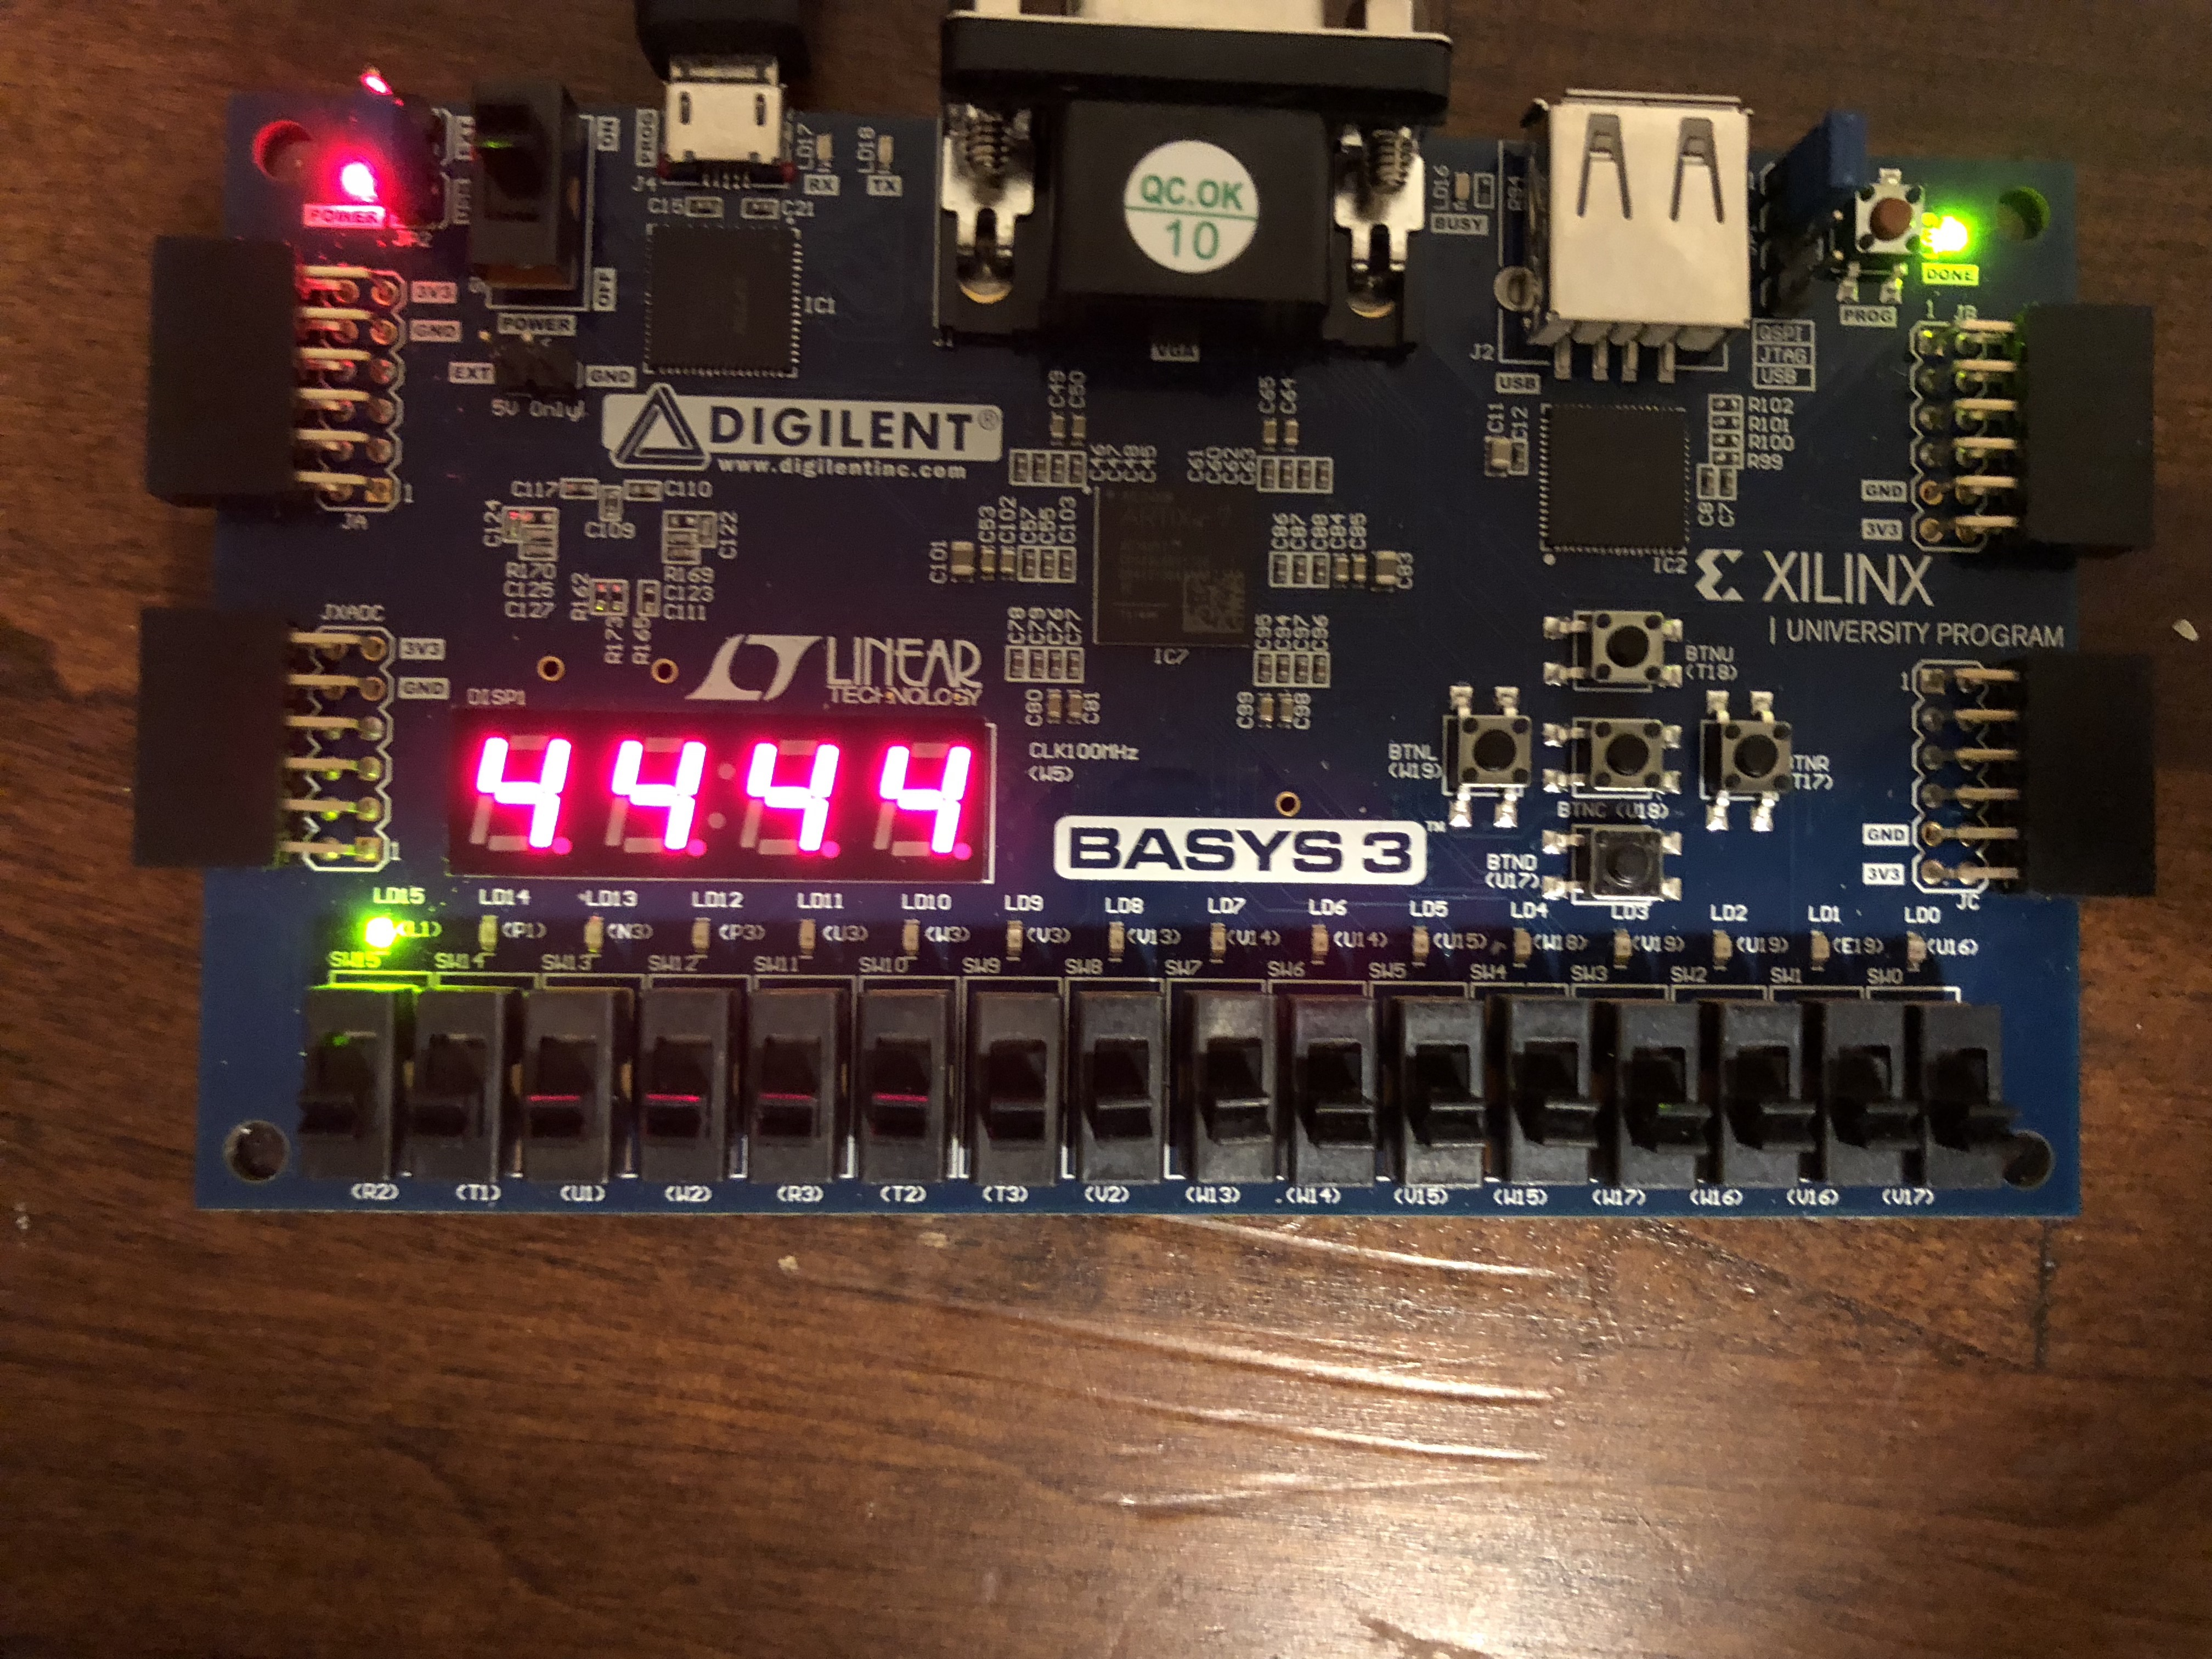
\includegraphics[width=0.5\textwidth]{./images/p1/IMG_1005.jpg}
	\caption{\label{fig:counter_res5}Counting down, at 4. Direction Switch 1 is off.}
\end{center}
\end{figure}

\begin{figure}[H]
\begin{center}
	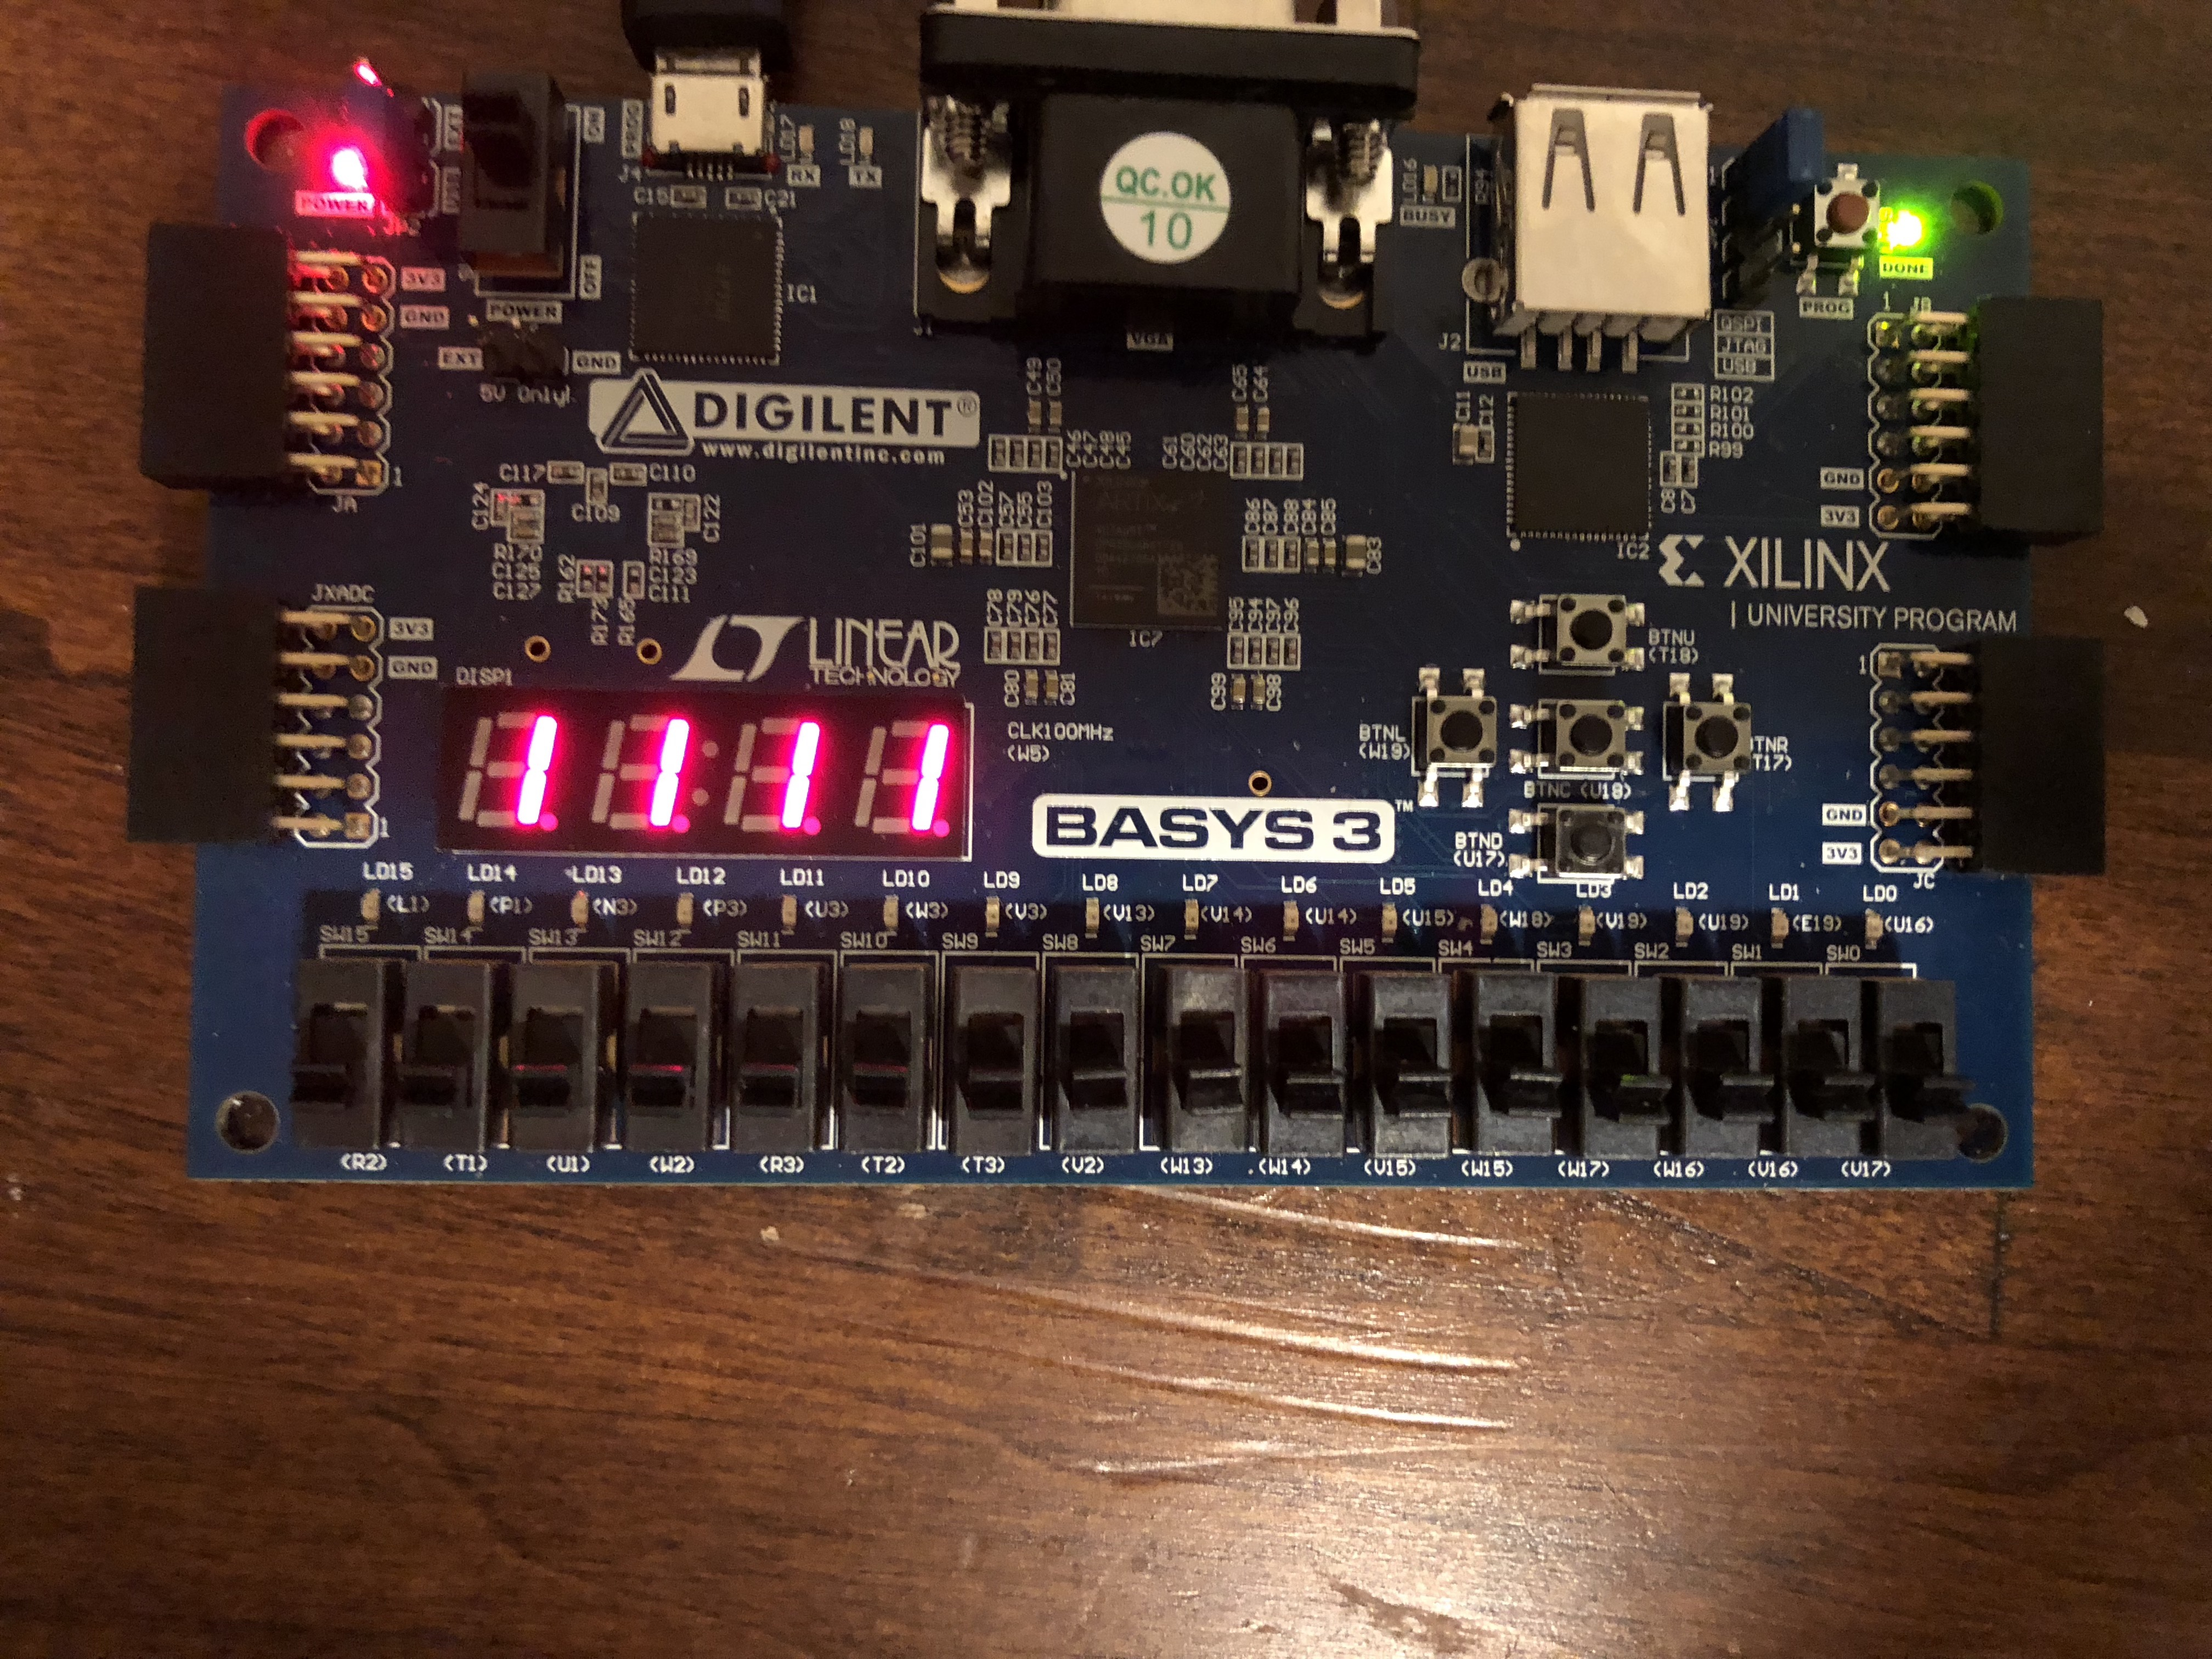
\includegraphics[width=0.5\textwidth]{./images/p1/IMG_1006.jpg}
	\caption{\label{fig:counter_res6}Counting down, at 1. Direction Switch 1 is off.}
\end{center}
\end{figure}

\subsection{Problem 2 }

\subsubsection{Background}
For Problem 2, we are required to add wrap-around functionality, load, enable, and synchronous reset to the counter from Problem 1.

\subsubsection{Design Solution}
Some functionality, such as reset and enable, already existed from the previous problem, where we found it easier to implement a synchronous design with these things than without them. For this problem, they just had to be given input ports. The input ports are summarized in Table ~\ref{tab:advanced_counter_input_Ports} and the output ports are summarized in ~\ref{tab:advanced_counter_output_Ports}. For the load operation, we decided to accept a 4-bit number so that we could inititalize the counter to any value that it could normally count to, 0 through 9. Any value greater than 9 ("1001") automatically results in the counter being set to 0.

\begin{table}[H]
\begin{center}
\begin{tabular}{| l | l | l |}
	\hline
	Bit & Label & Port \\ \hline
	clk &  Clock & W5 \\ \hline
	direction & Switch 0 & V17 \\ \hline
	load & Switch 1 & V16 \\ \hline
	enable & Switch 2 & W16 \\ \hline
	reset & Button Right & T17 \\ \hline
	input3 & Switch 15 & R2 \\ \hline
	input2 & Switch 14 & T1 \\ \hline
	input1 & Switch 13 & U1 \\ \hline
	input 0 & Switch 12 & W2 \\ \hline
\end{tabular}
\caption{\label{tab:advanced_counter_input_Ports}Input port assignments for  the advanced counter.}
\end{center}
\end{table}

\begin{table}[H]
\begin{center}
\begin{tabular}{| l | l | l |}
	\hline
	Bit & Label & Port \\ \hline
	clk led & LED 15 & L1 \\ \hline
	count6 & CA & W7 \\ \hline
	count5 & CB & W6 \\ \hline
	count4 & CC & U8 \\ \hline
	count3 & CD & V8 \\ \hline
	count2 & CE & U5 \\ \hline
	count1 & CF & V5 \\ \hline
	count0 & CG & U7 \\ \hline
\end{tabular}
\caption{\label{tab:advanced_counter_output_Ports}Output port assignments for the advanced counter.}
\end{center}
\end{table}


\subsubsection{Results}
The counter was able to successfully load values and pause when disabled. Selected photographs are shown in Figures ~\ref{fig:advanced_counter_res1} through ~\ref{fig:advanced_counter_res7}.

\begin{figure}[H]
\begin{center}
	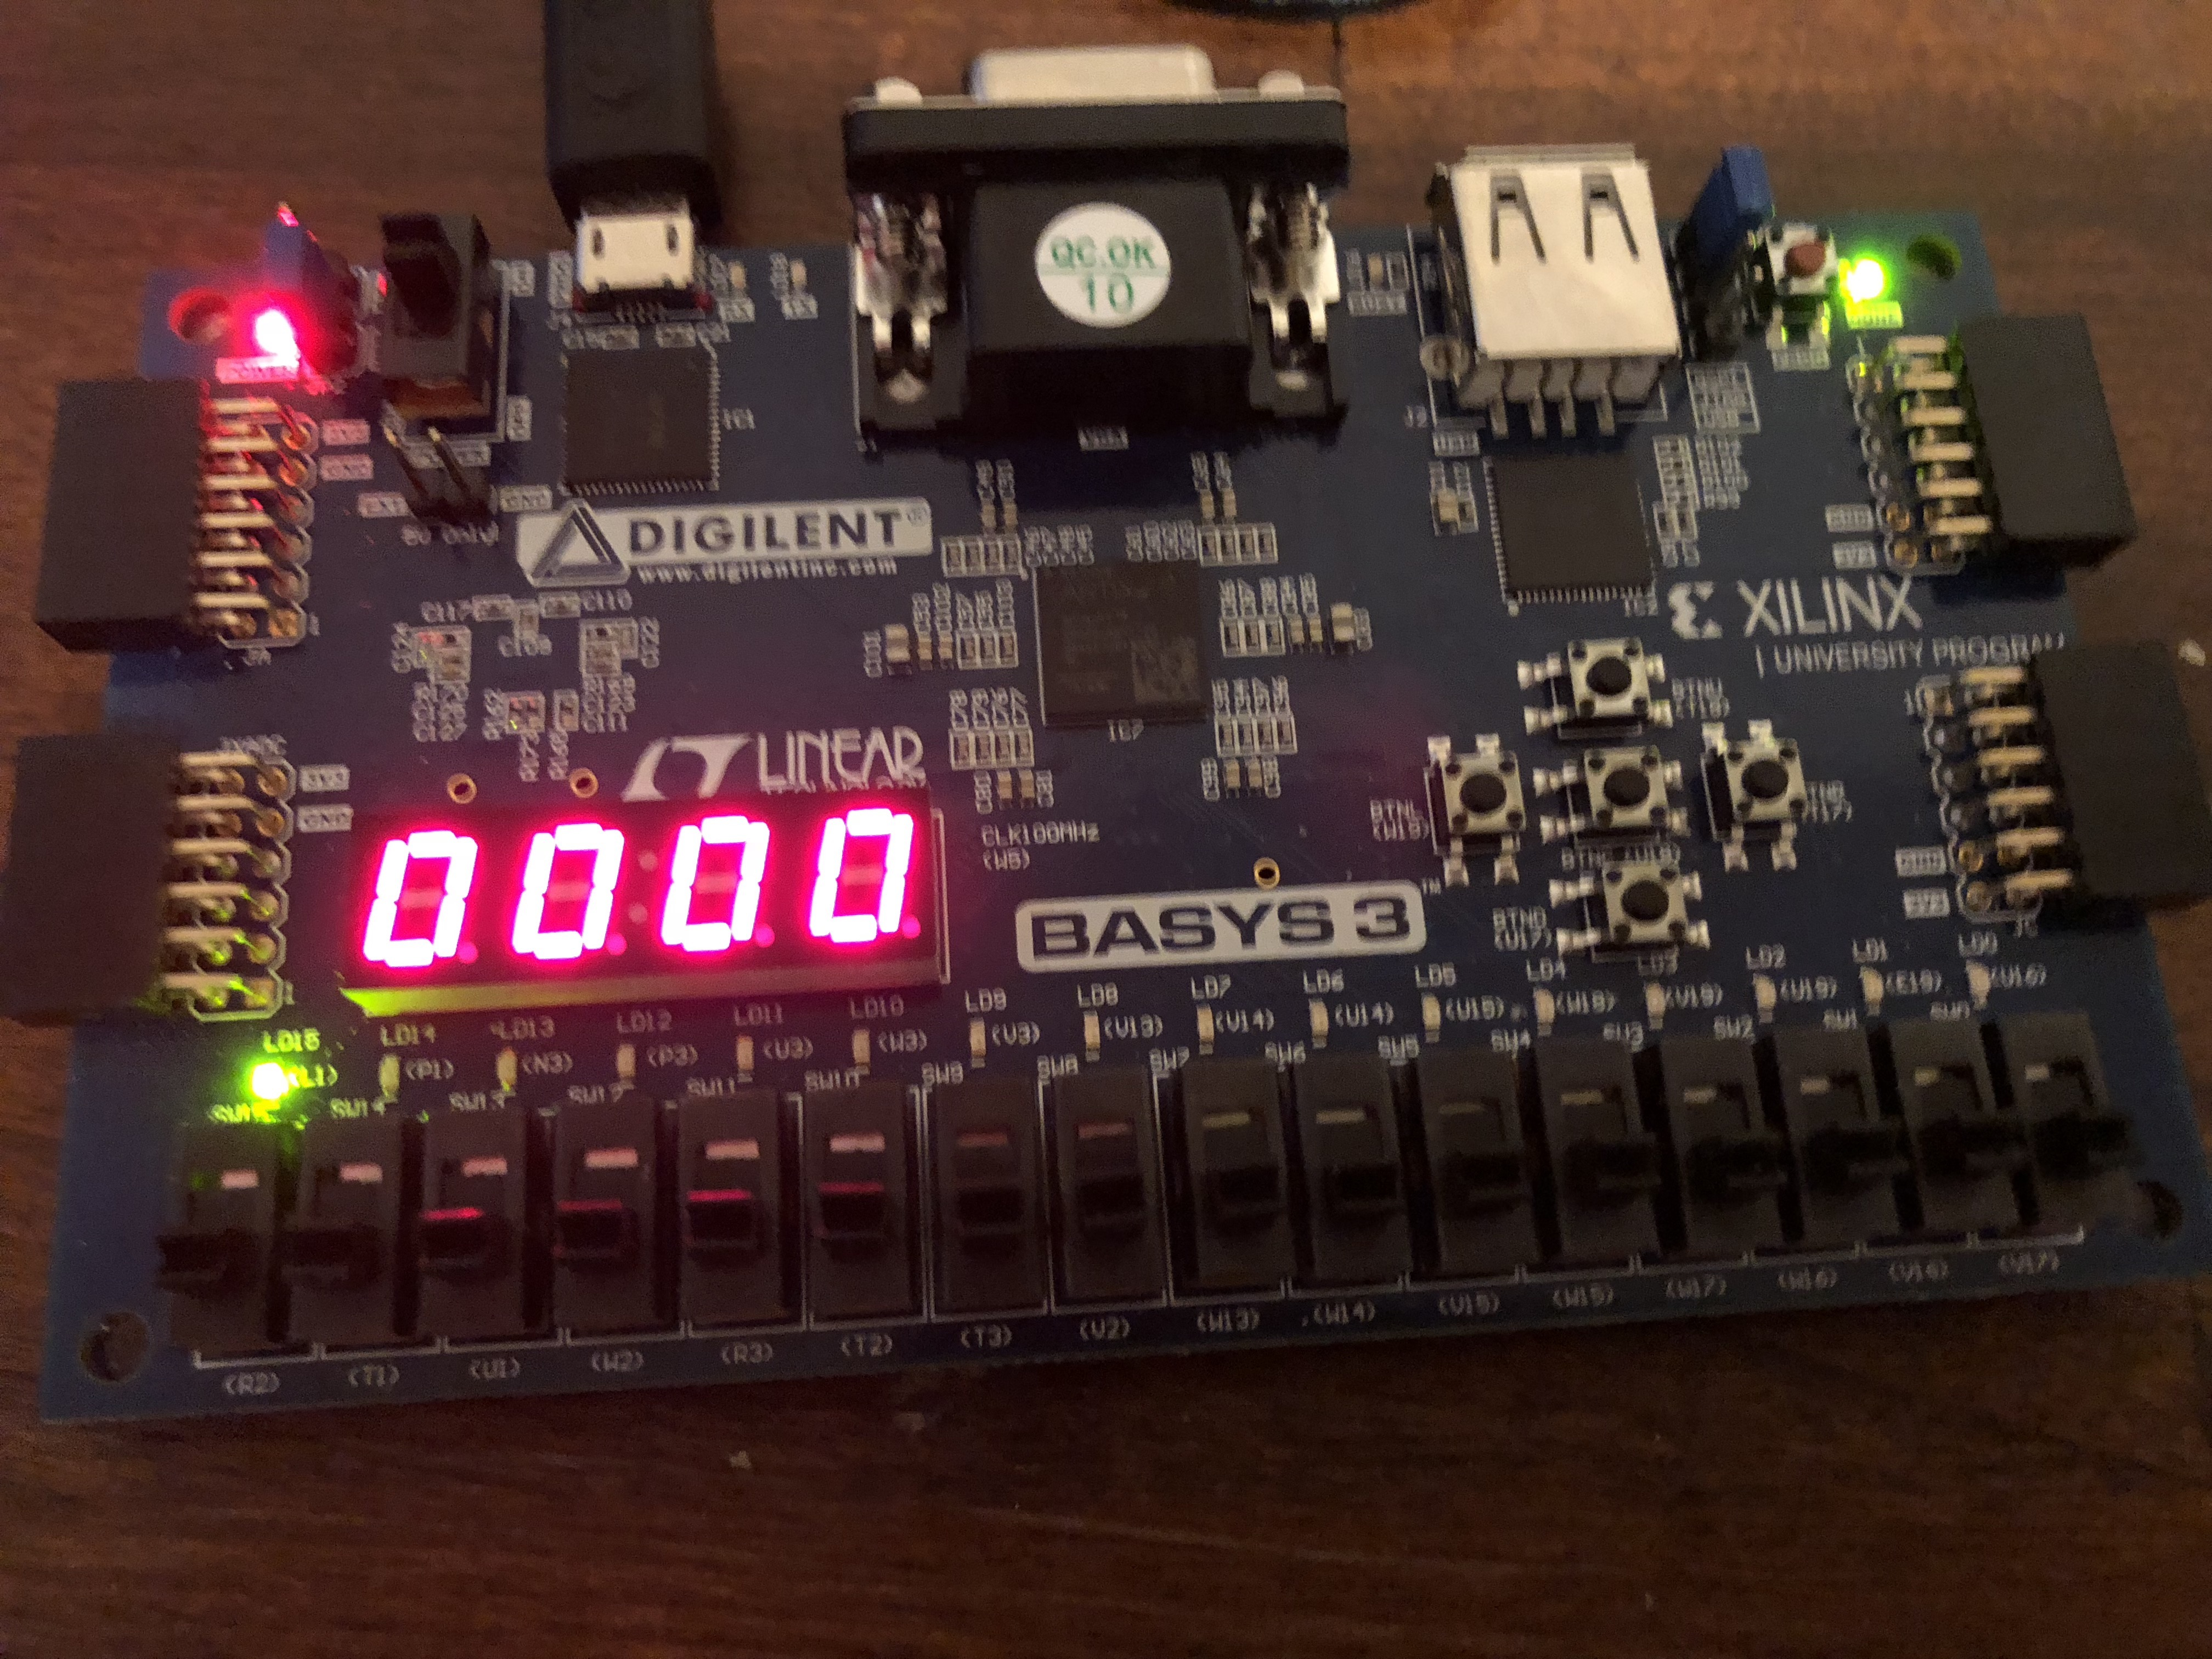
\includegraphics[width=0.5\textwidth]{./images/p2/IMG_1007.jpg}
	\caption{\label{fig:advanced_counter_res1}Disabled, meaning that the counter will retain the value 0 until it is told to count again.}
\end{center}
\end{figure}

\begin{figure}[H]
\begin{center}
	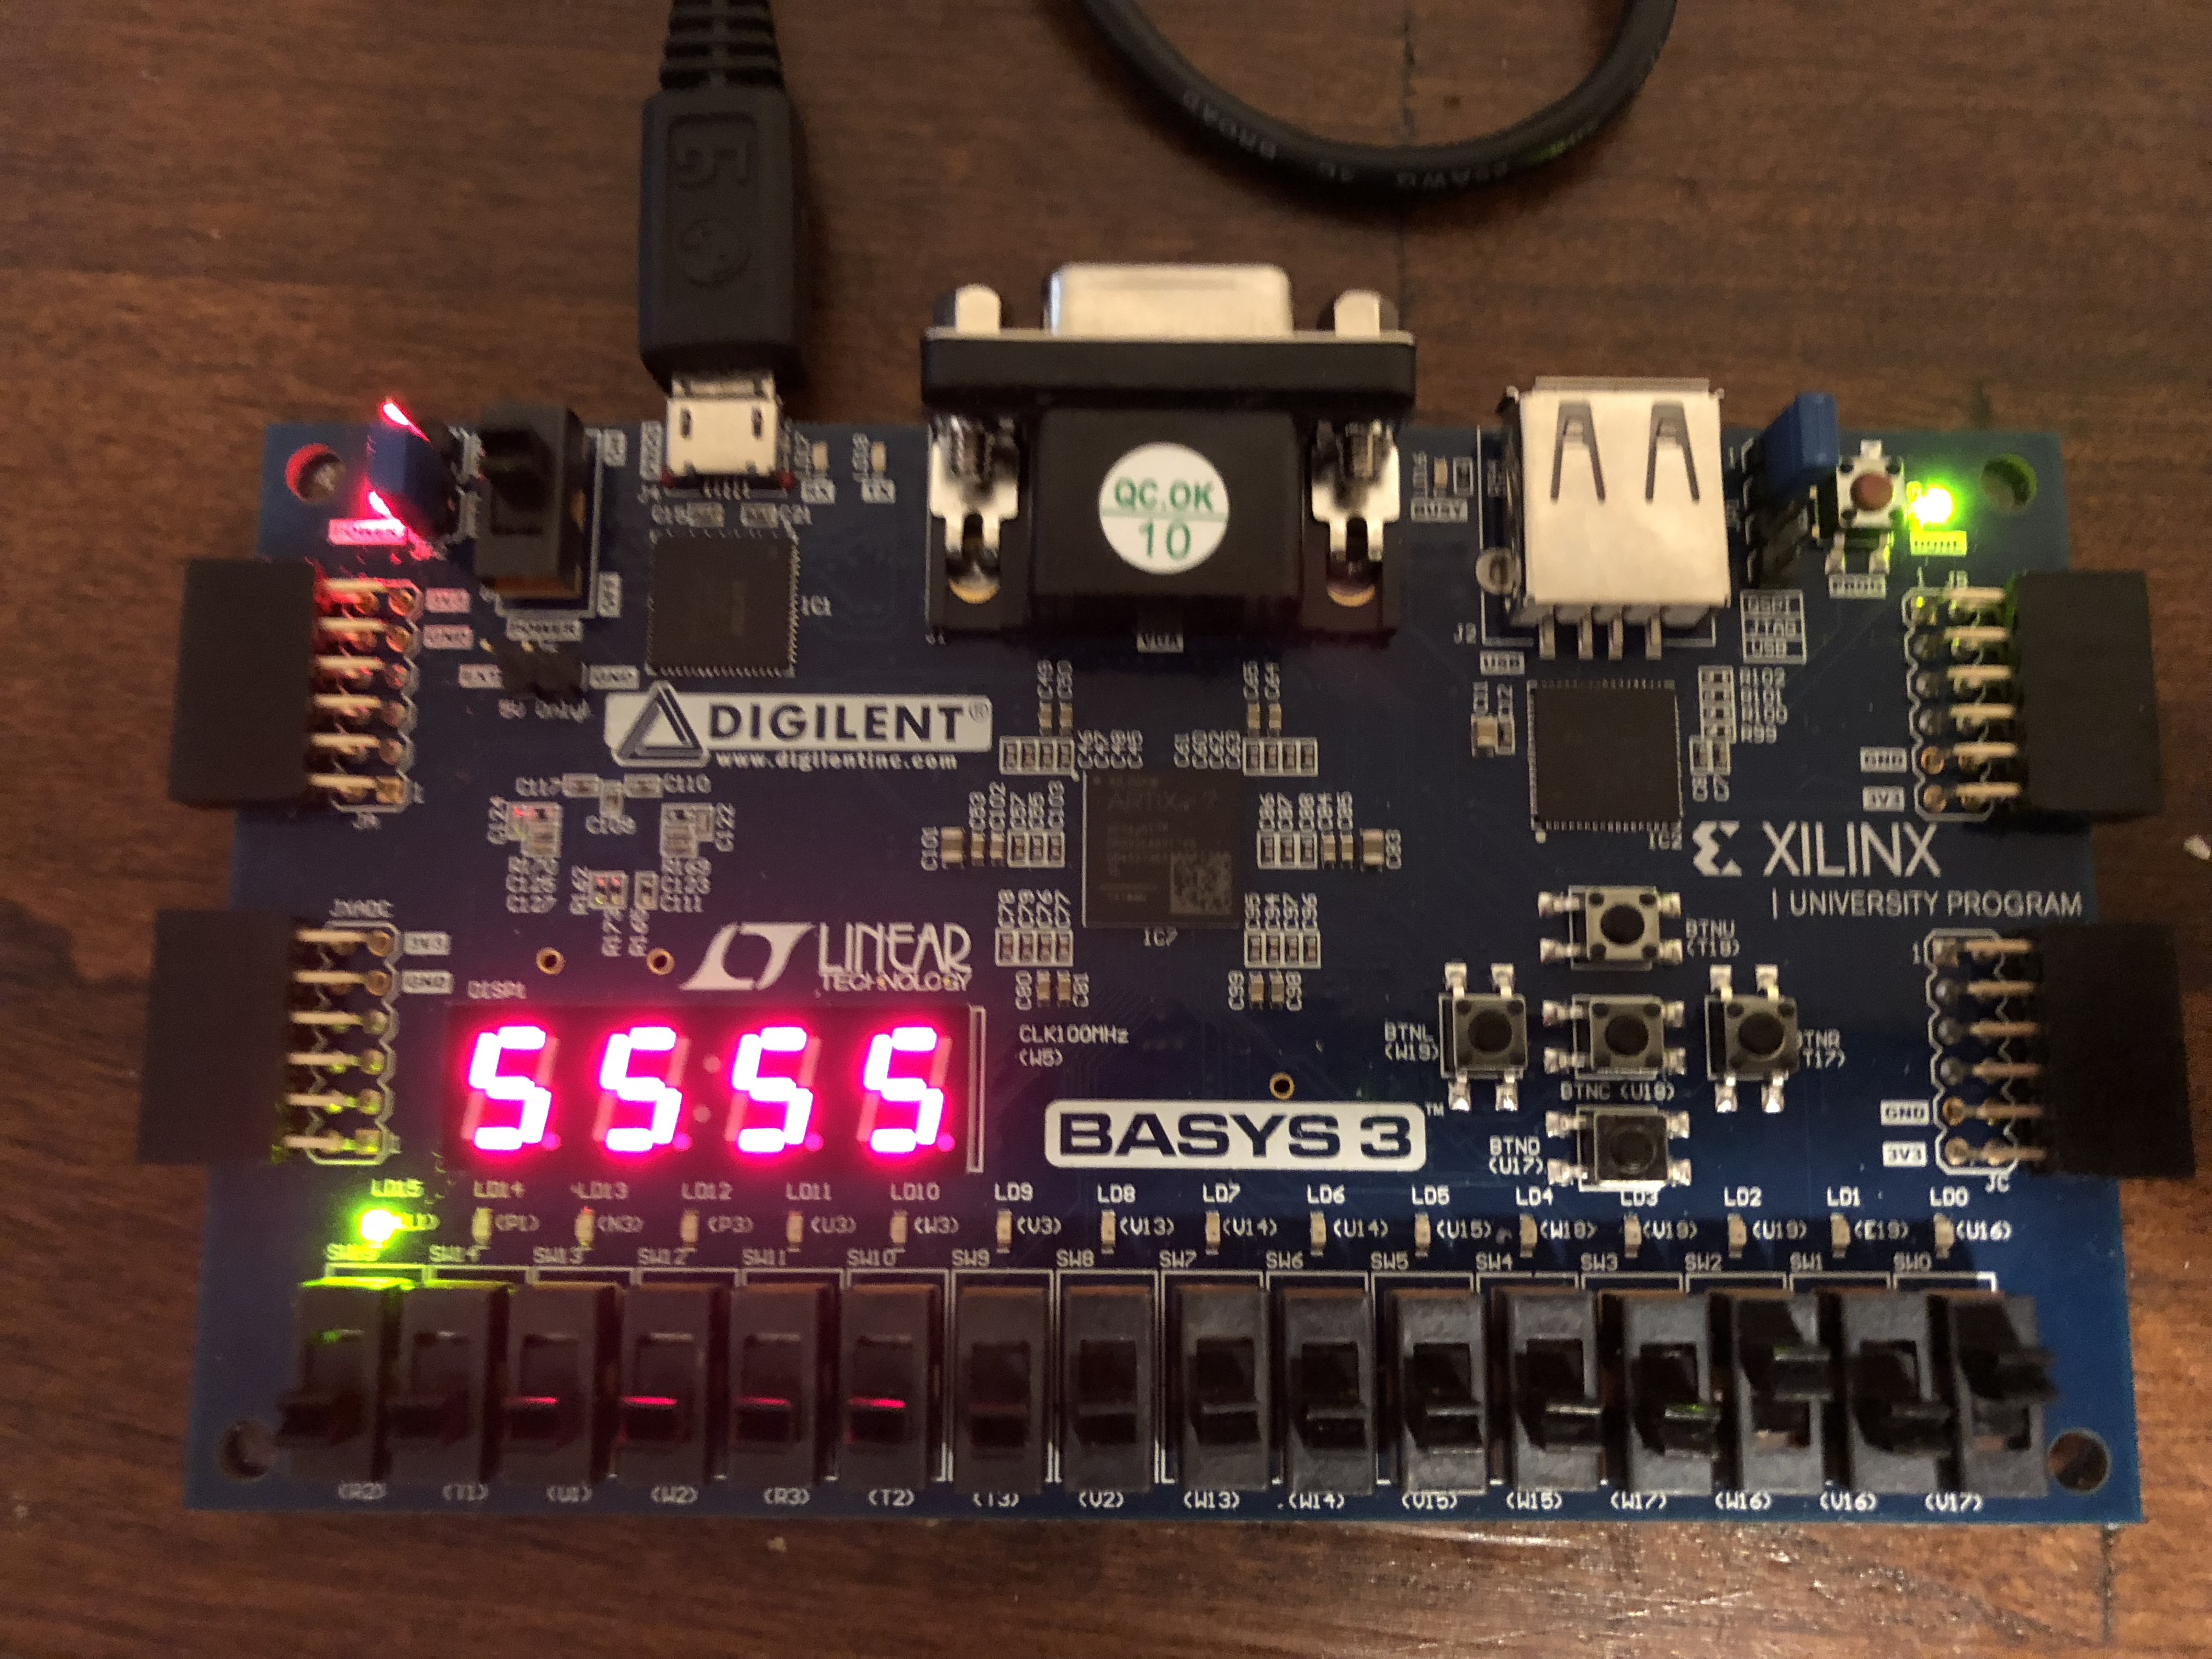
\includegraphics[width=0.5\textwidth]{./images/p2/IMG_1008.jpg}
	\caption{\label{fig:advanced_counter_res2}Enabled and counting up.}
\end{center}
\end{figure}

\begin{figure}[H]
\begin{center}
	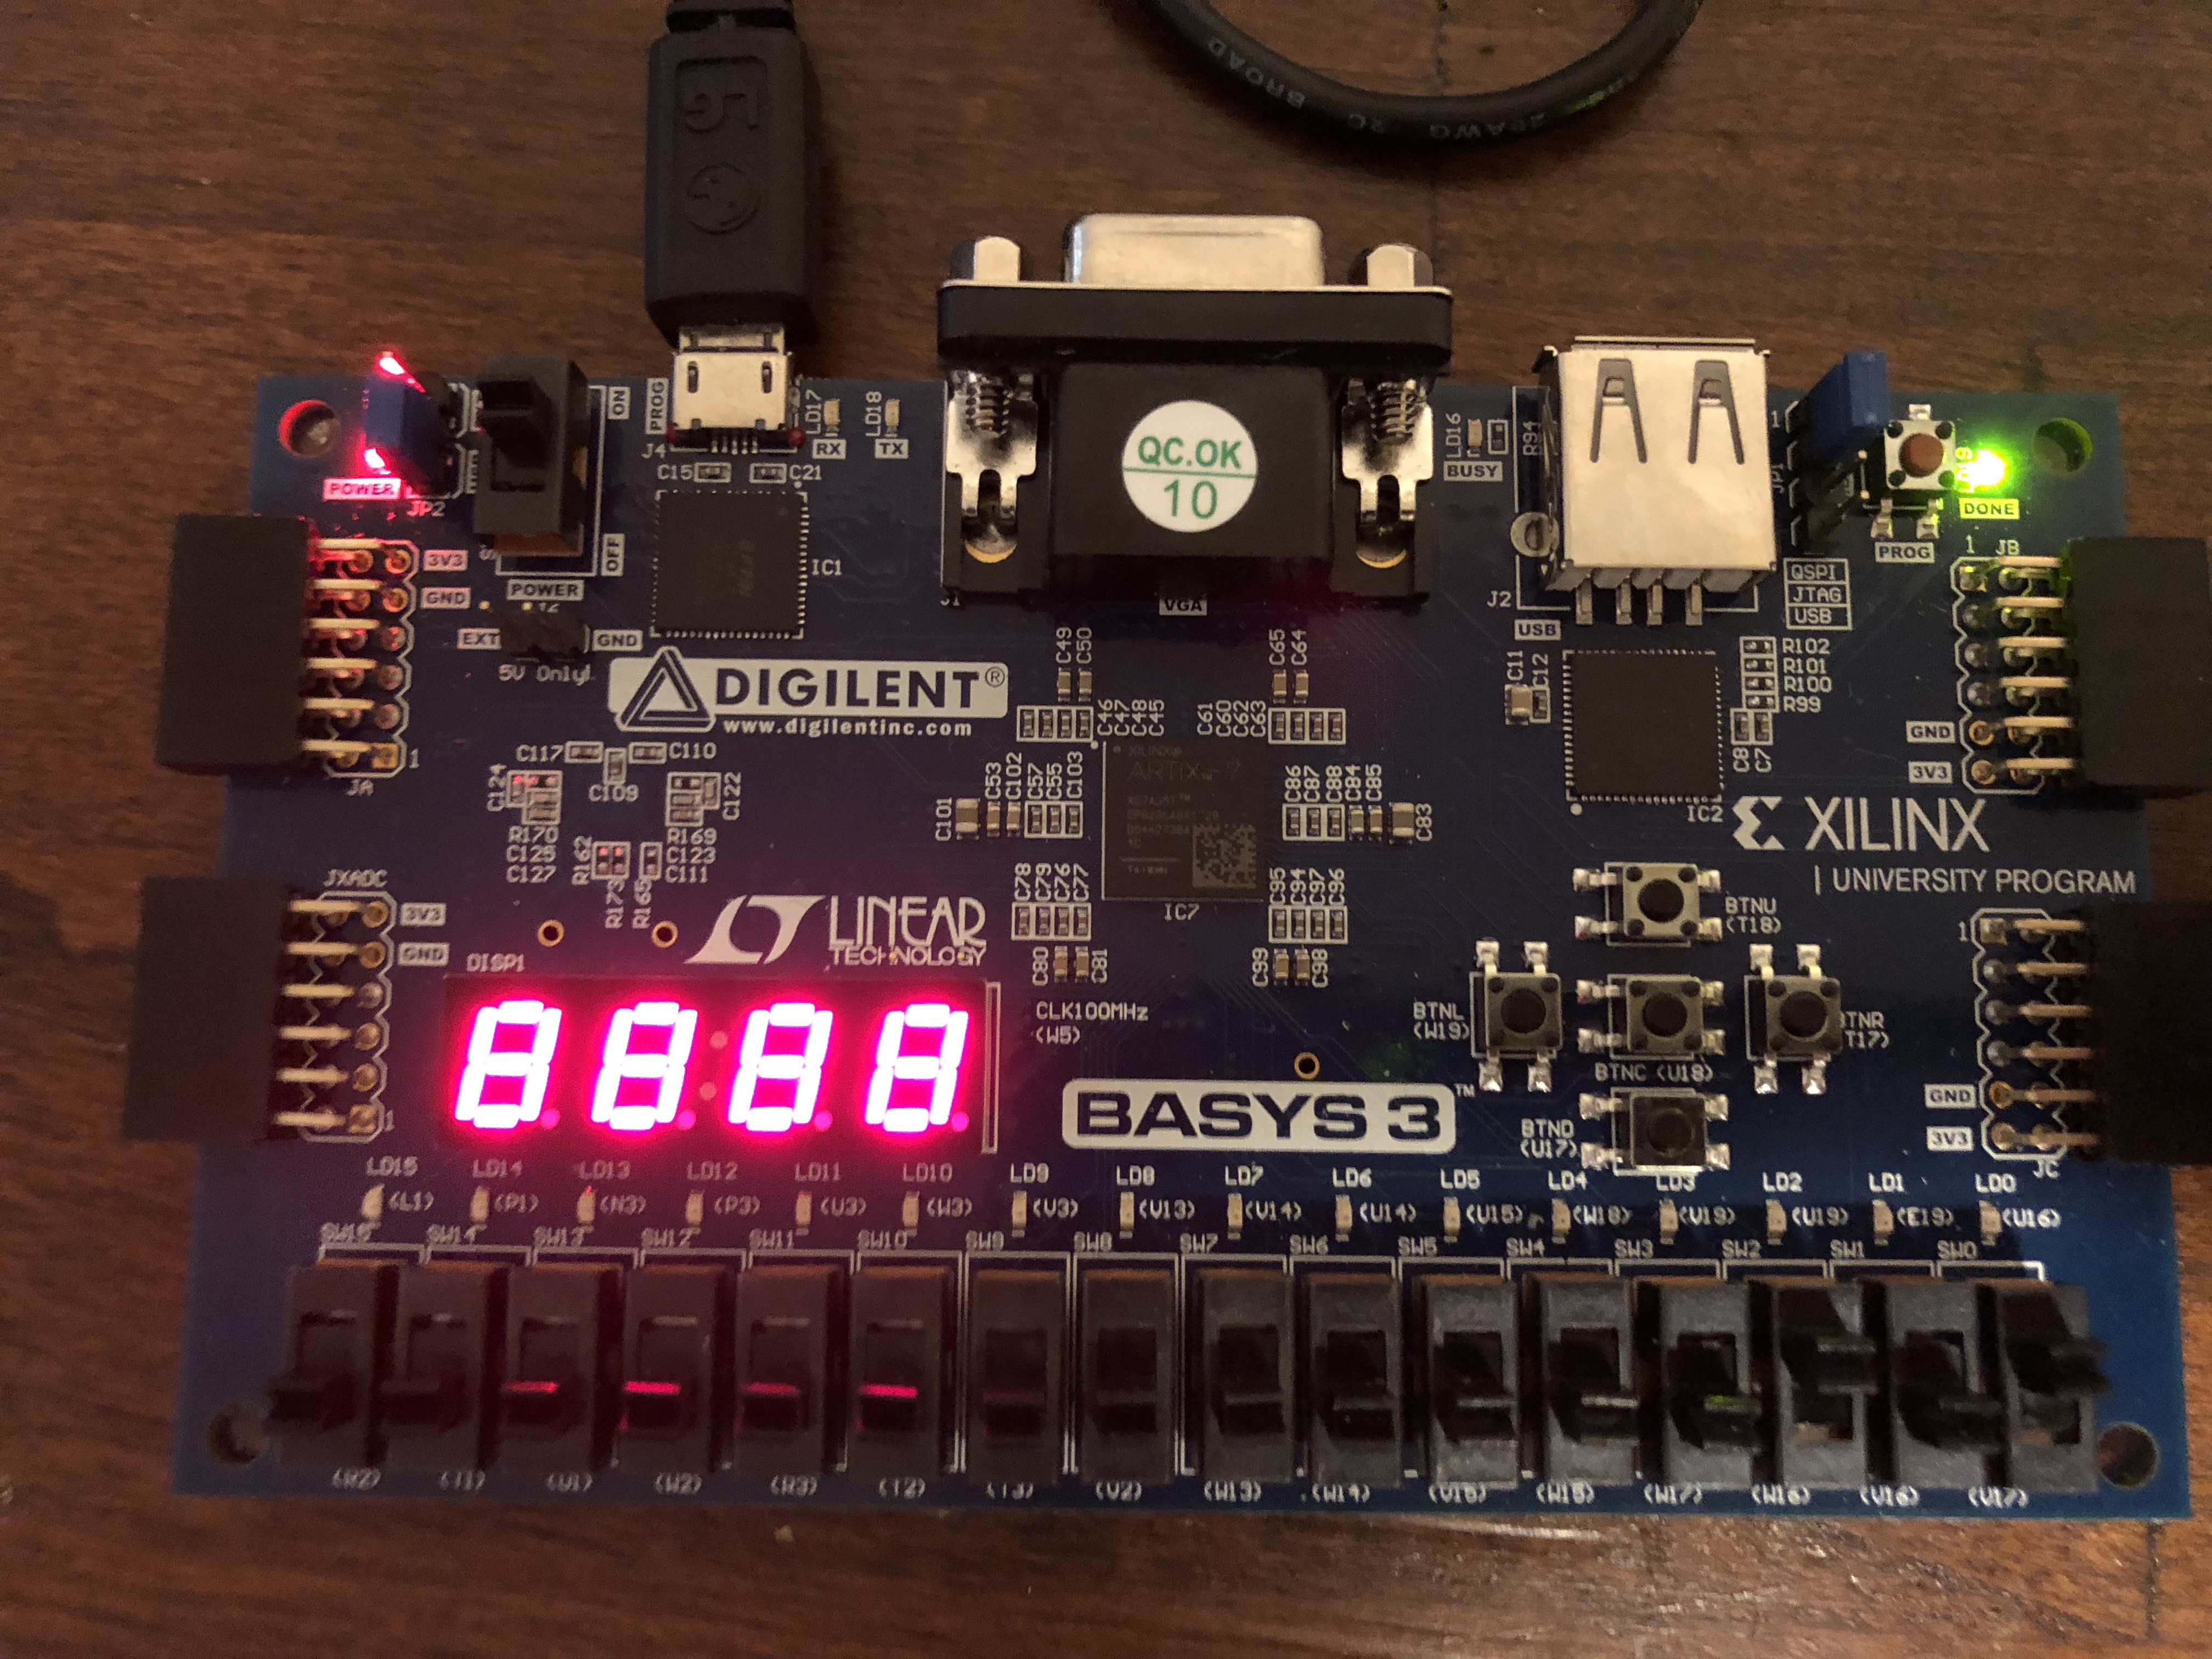
\includegraphics[width=0.5\textwidth]{./images/p2/IMG_1009.jpg}
	\caption{\label{fig:advanced_counter_res3}Enabled and counting up.}
\end{center}
\end{figure}

\begin{figure}[H]
\begin{center}
	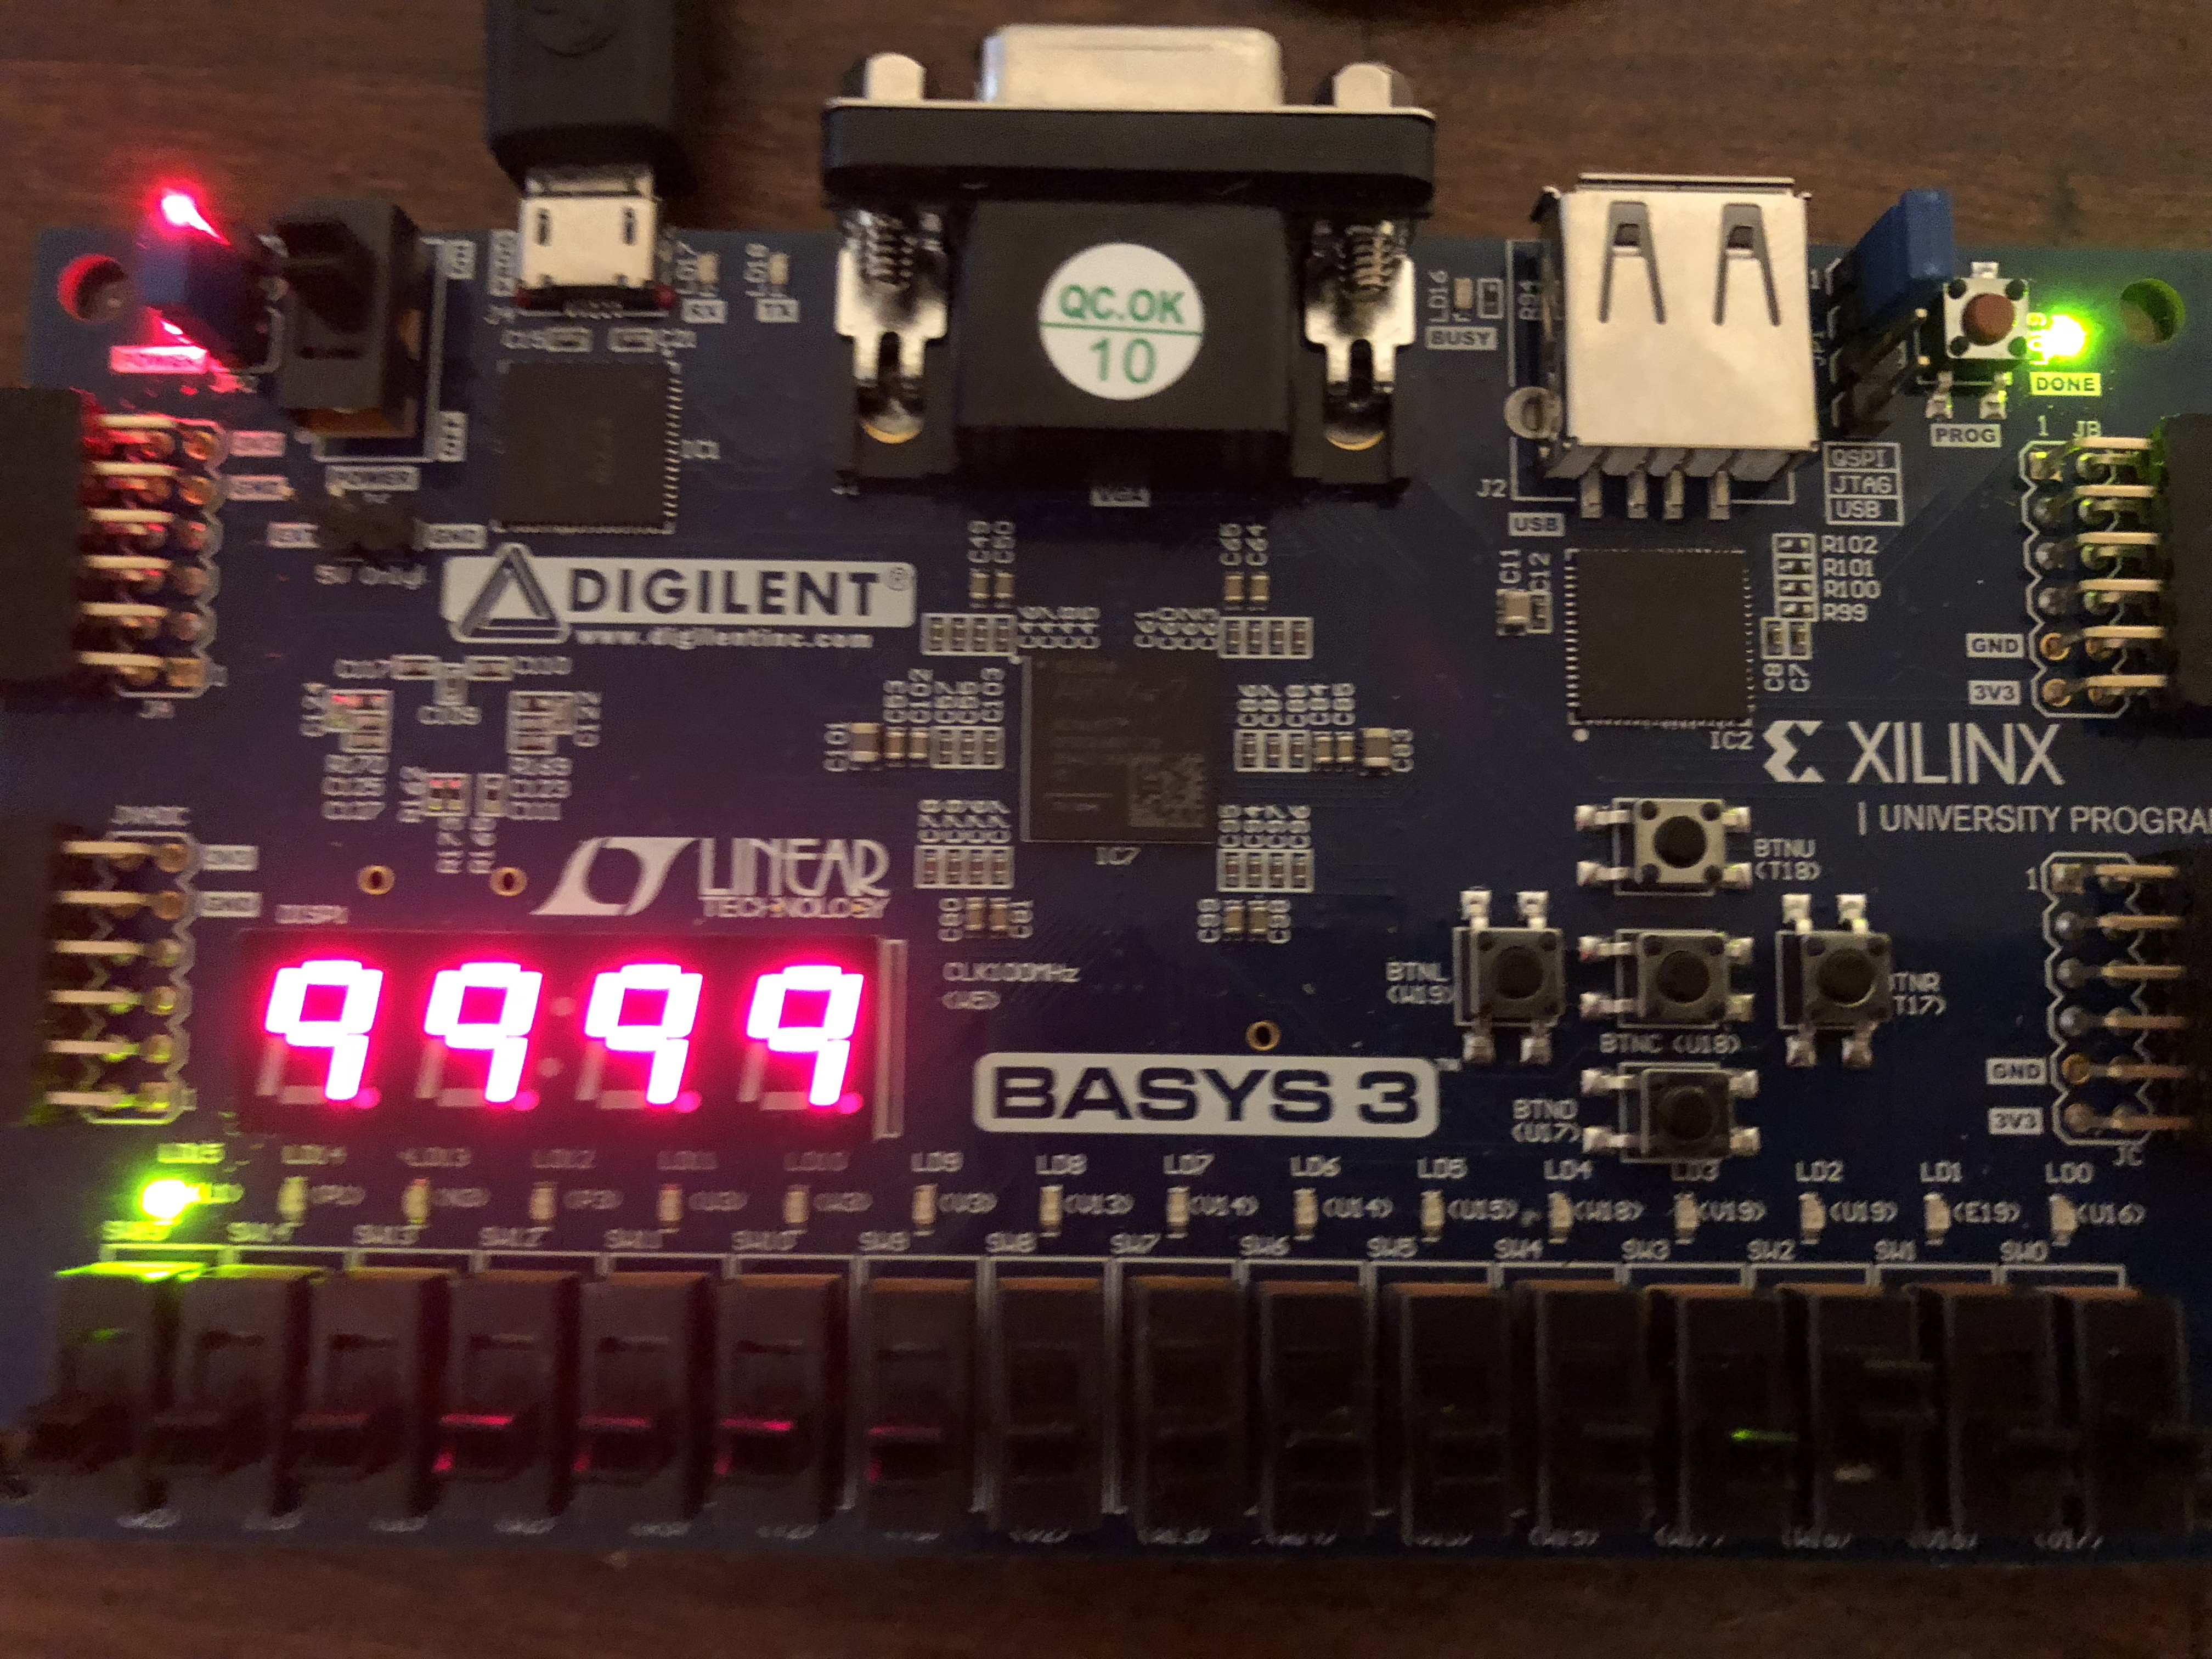
\includegraphics[width=0.5\textwidth]{./images/p2/IMG_1010.jpg}
	\caption{\label{fig:advanced_counter_res4}Enabled and counting down, which means the counter has just transitioned from 0 to 9 because of the wrap-around functionality.}
\end{center}
\end{figure}

\begin{figure}[H]
\begin{center}
	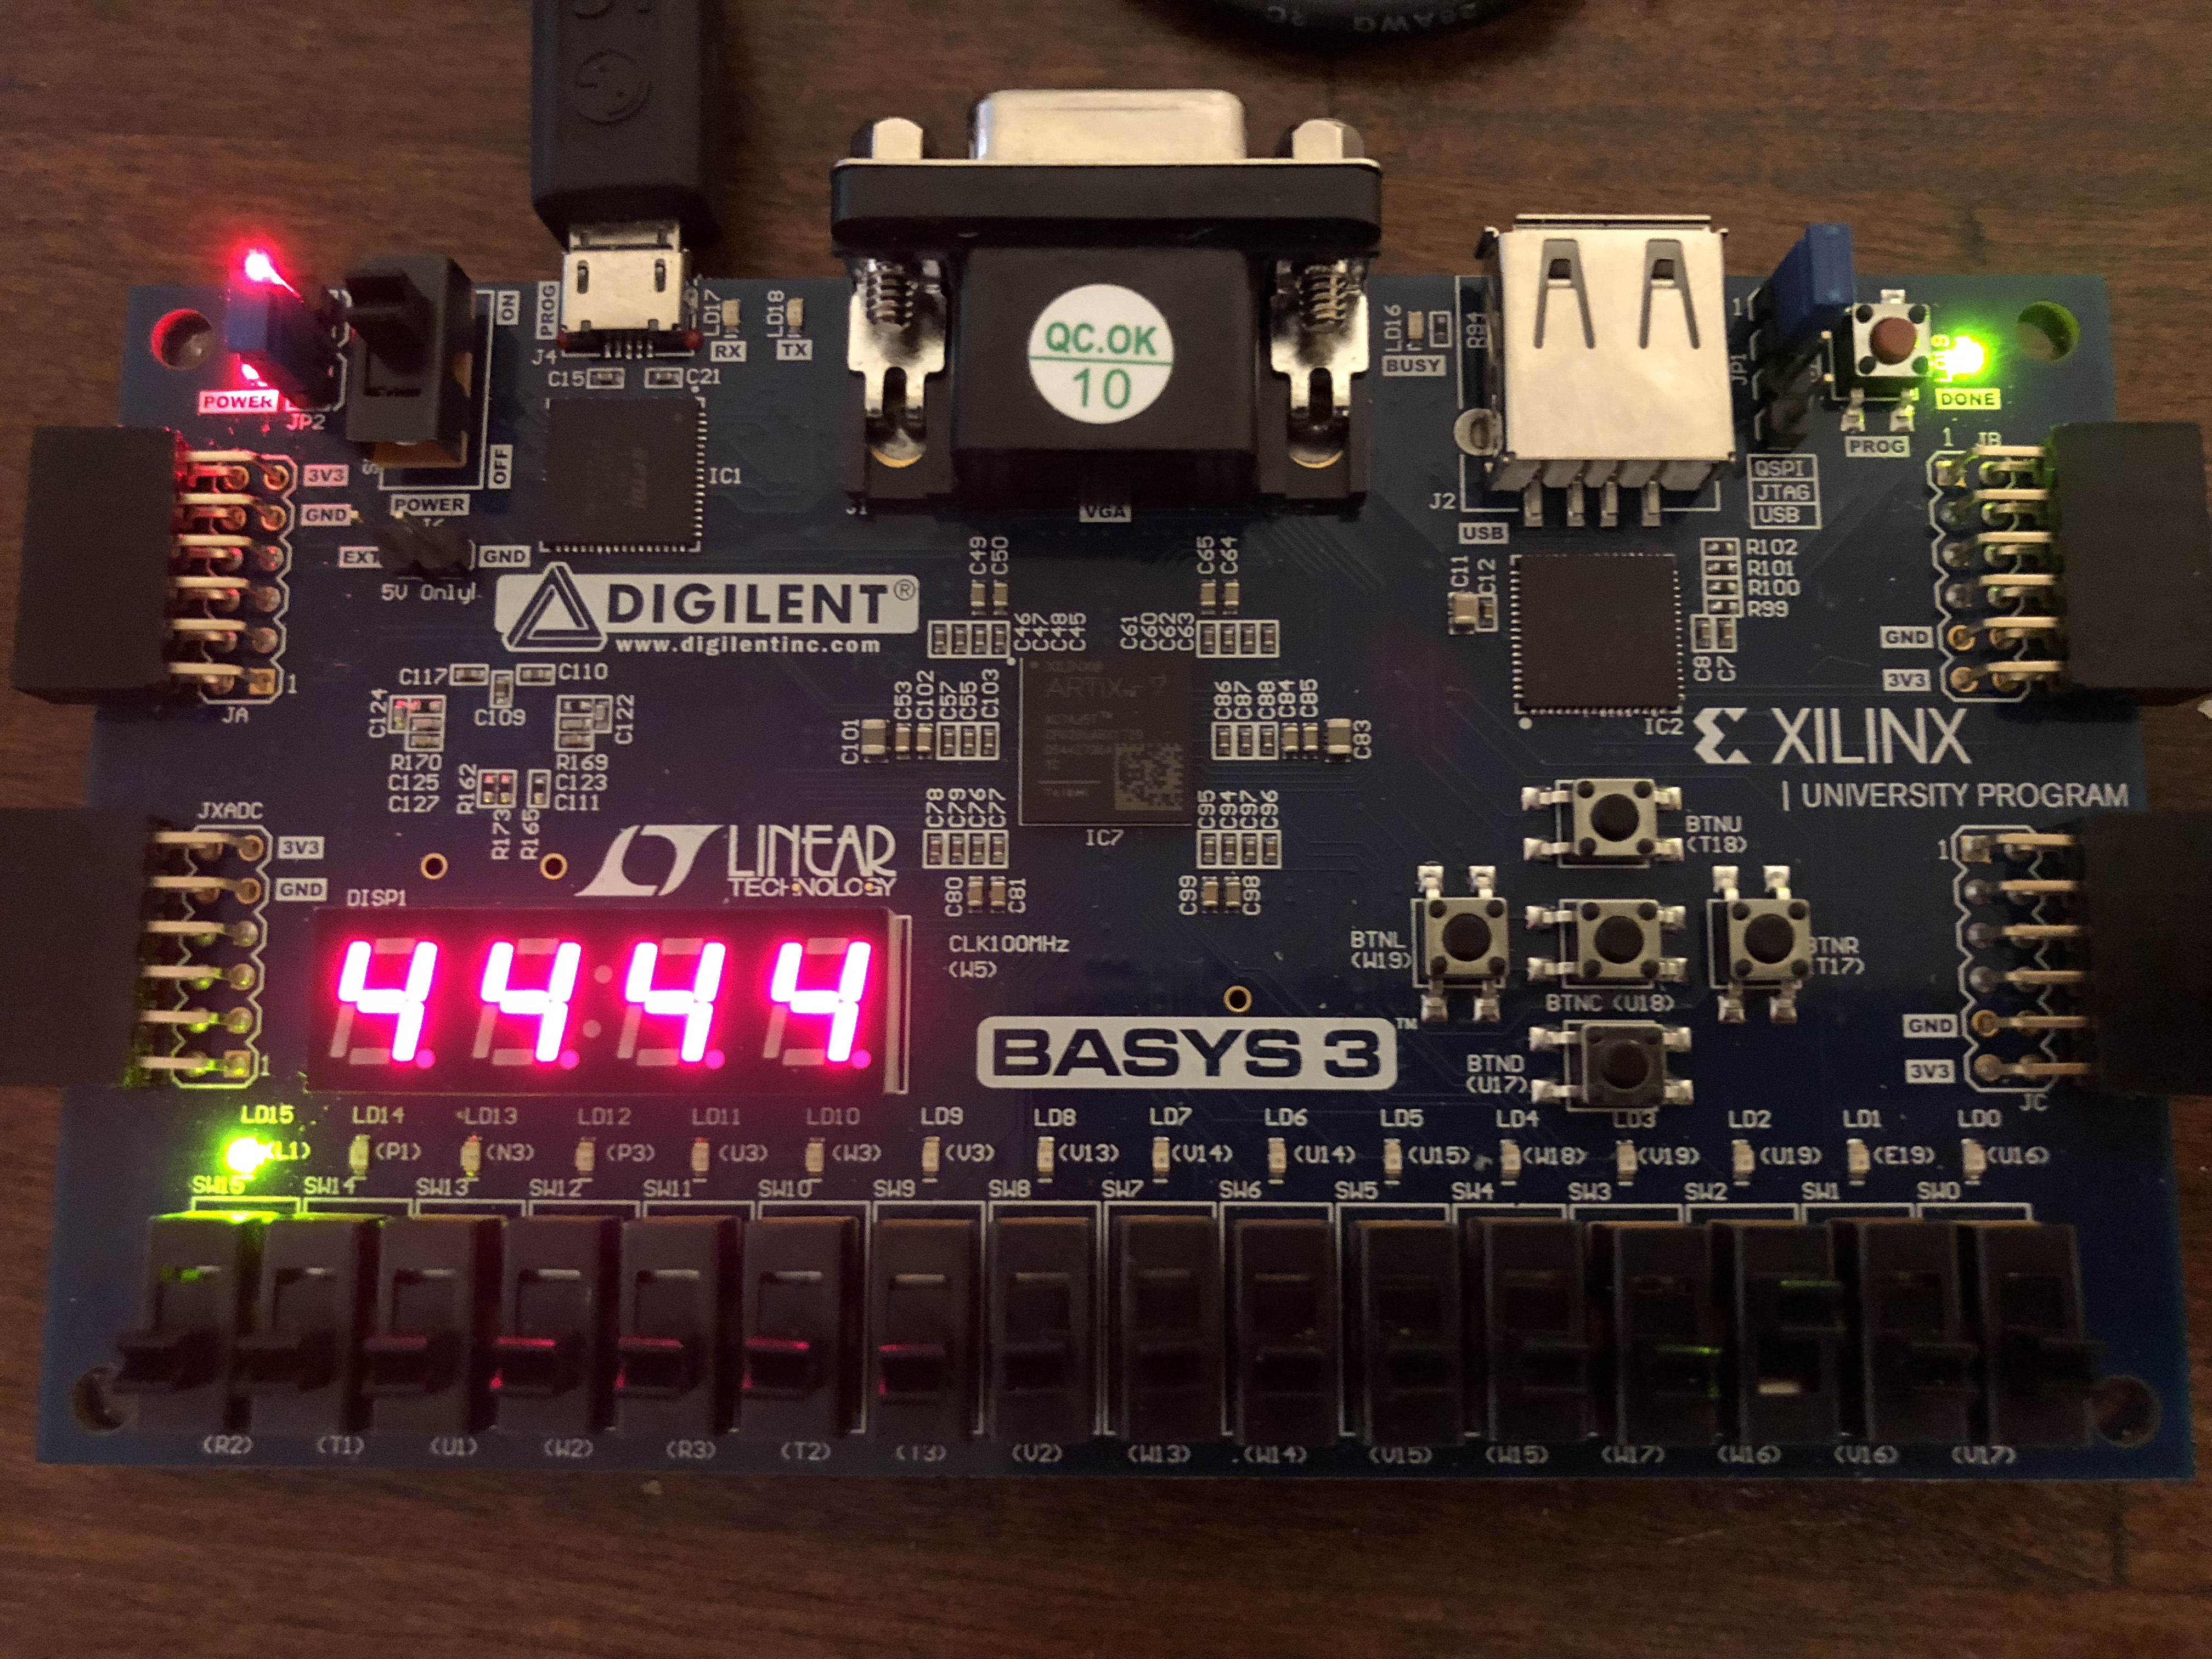
\includegraphics[width=0.5\textwidth]{./images/p2/IMG_1011.jpg}
	\caption{\label{fig:advanced_counter_res5}Enabled and counting down.}
\end{center}
\end{figure}

\begin{figure}[H]
\begin{center}
	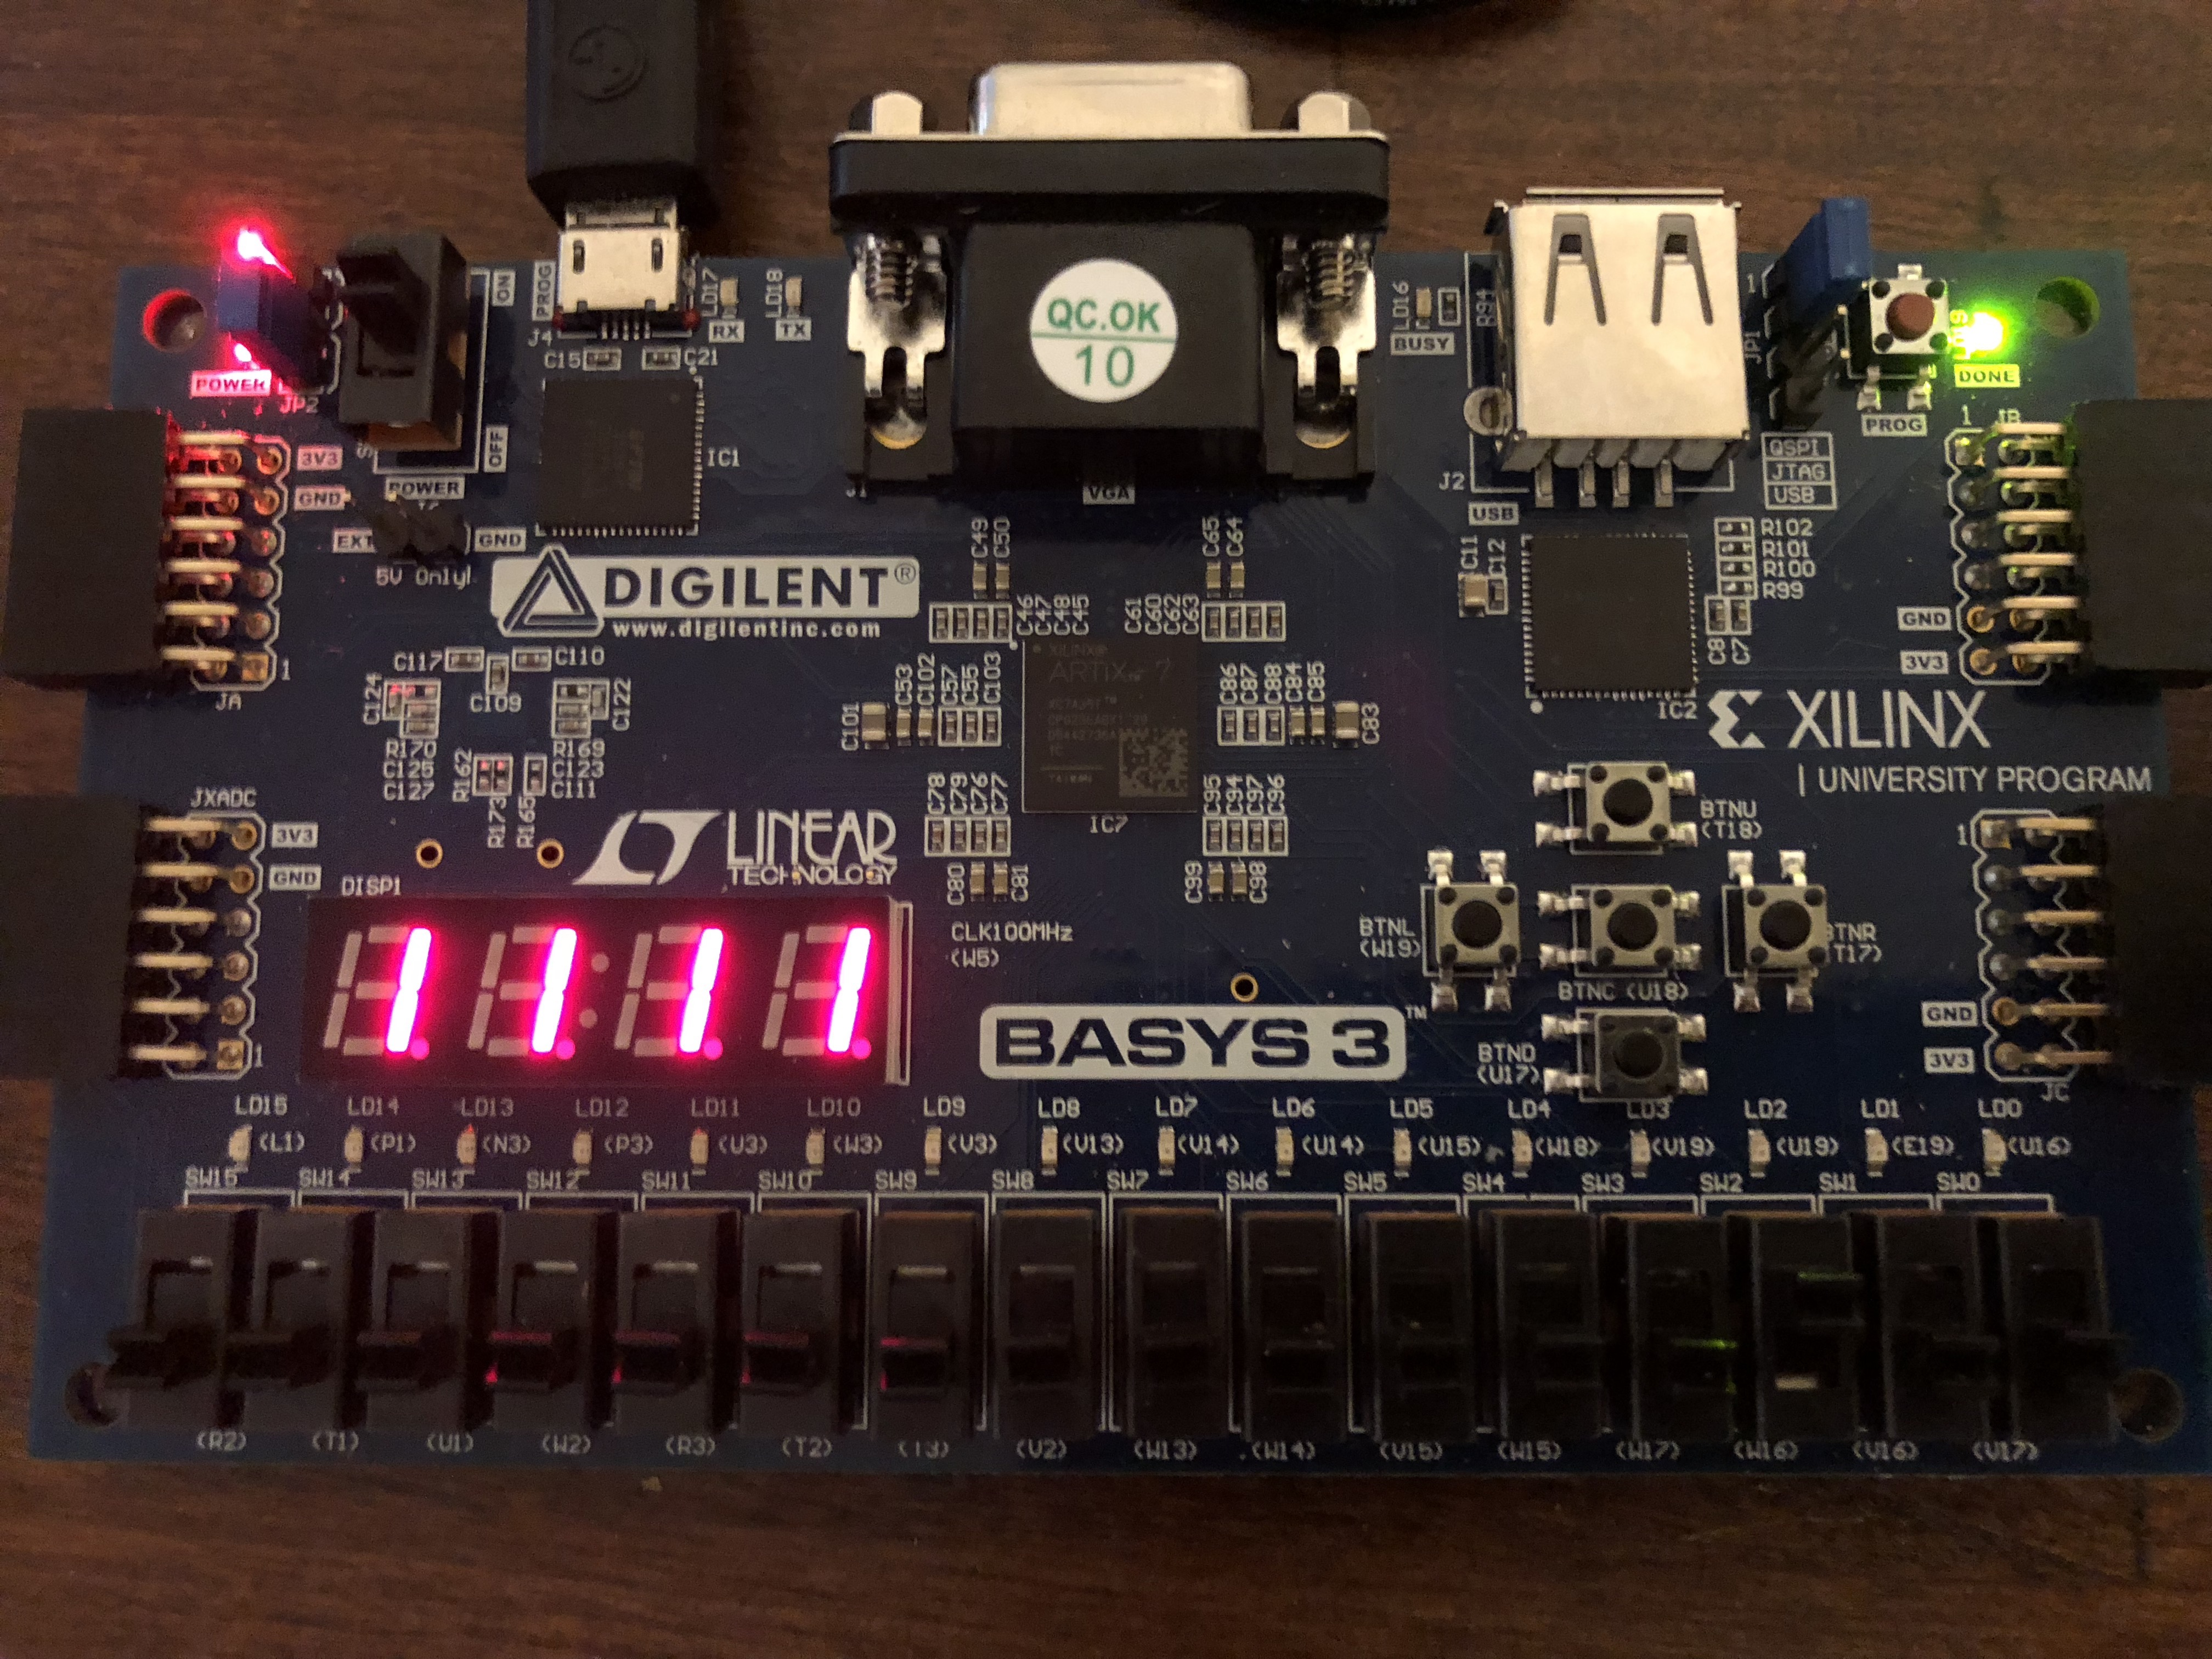
\includegraphics[width=0.5\textwidth]{./images/p2/IMG_1012.jpg}
	\caption{\label{fig:advanced_counter_res6}Enabled and counting down.}
\end{center}
\end{figure}

\begin{figure}[H]
\begin{center}
	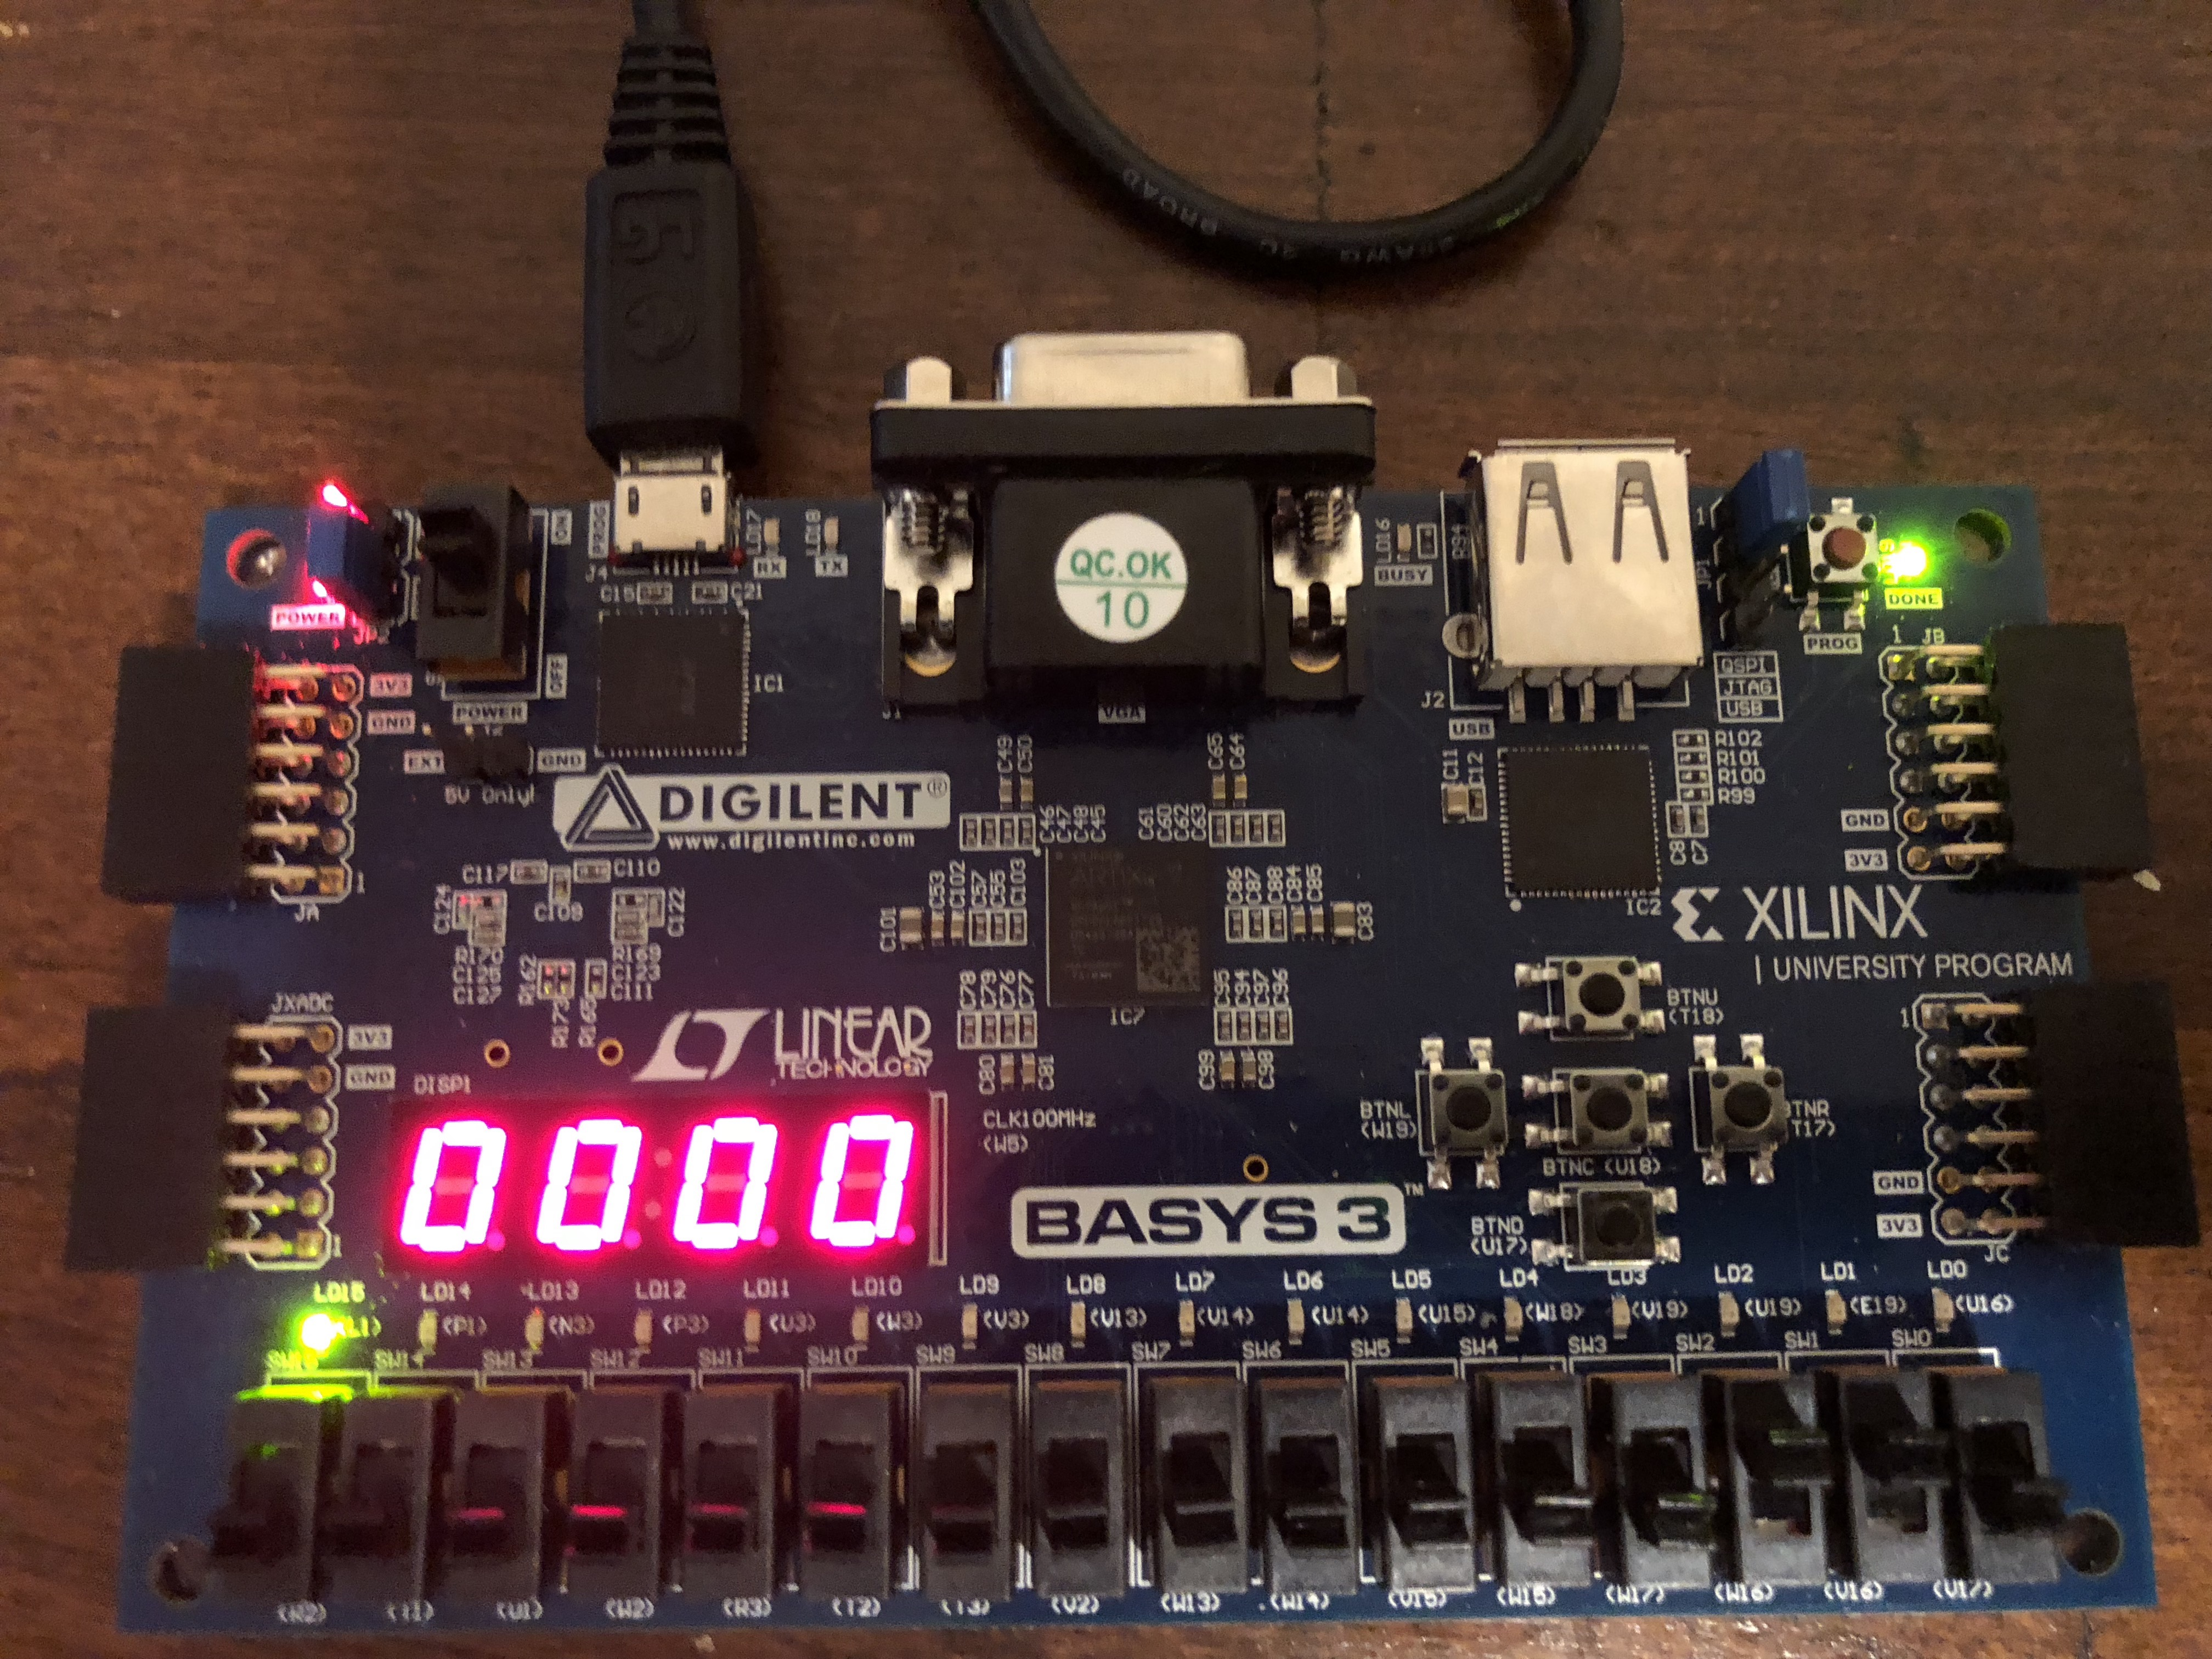
\includegraphics[width=0.5\textwidth]{./images/p2/IMG_1013.jpg}
	\caption{\label{fig:advanced_counter_res7}Enabled and instructed to load a value of "0000". Therefore, on every clock edge the counter is set back to 0.}
\end{center}
\end{figure}

\subsection{Problem 3}

\subsubsection{Background}
For Problem 3, we were to detect input sequences using a finite state machine that would change direction of the counter. There would be no other required interaction with the counter except by the reset.

\subsubsection{Design Solution}
We selected the sequence "101" to tell our machine to count up and "010" to tell our machine to count down. The state machine is shown in Figure ~\ref{fig:state_diagram}. We decided to have our counter go down by default. The input ports are summarized in Table ~\ref{tab:integration_input_Ports} and the output ports in Table ~\ref{tab:integration_output_Ports}. We decided to retain all capabilities of the previous problem such as load.

\begin{figure}[H]
\begin{center}
	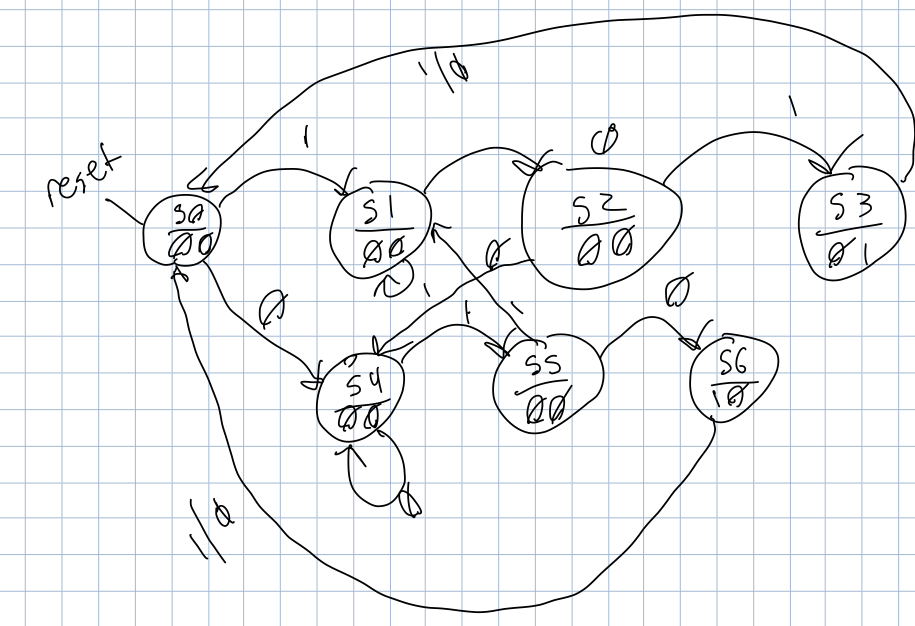
\includegraphics[width=0.5\textwidth]{./images/statediagram.png}
	\caption{\label{fig:state_diagram}}
\end{center}
\end{figure}

\begin{table}[H]
\begin{center}
\begin{tabular}{| l | l | l |}
	\hline
	Bit & Label & Port \\ \hline
	clk &  Clock & W5 \\ \hline
	direction & Switch 0 & V17 \\ \hline
	load & Switch 1 & V16 \\ \hline
	enable & Switch 2 & W16 \\ \hline
	reset & Button Right & T17 \\ \hline
	input3 & Switch 15 & R2 \\ \hline
	input2 & Switch 14 & T1 \\ \hline
	input1 & Switch 13 & U1 \\ \hline
	input 0 & Switch 12 & W2 \\ \hline
	state input & Button C & U18 \\ \hline
\end{tabular}
\caption{\label{tab:integration_input_Ports}Input port assignments for  the integrated circuit.}
\end{center}
\end{table}

\begin{table}[H]
\begin{center}
\begin{tabular}{| l | l | l |}
	\hline
	Bit & Label & Port \\ \hline
	clk led & LED 15 & L1 \\ \hline
	count6 & CA & W7 \\ \hline
	count5 & CB & W6 \\ \hline
	count4 & CC & U8 \\ \hline
	count3 & CD & V8 \\ \hline
	count2 & CE & U5 \\ \hline
	count1 & CF & V5 \\ \hline
	count0 & CG & U7 \\ \hline
\end{tabular}
\caption{\label{tab:integration_output_Ports}Output port assignments for the integrated circuit.}
\end{center}
\end{table}

\subsubsection{Results}
The finite state machine was able to successfully detect input sequences and change counter direction accordingly. Selected outputs are shown in Figures ~\ref{fig:int_res1} through ~\ref{fig:int_res6}.

\begin{figure}[H]
\begin{center}
	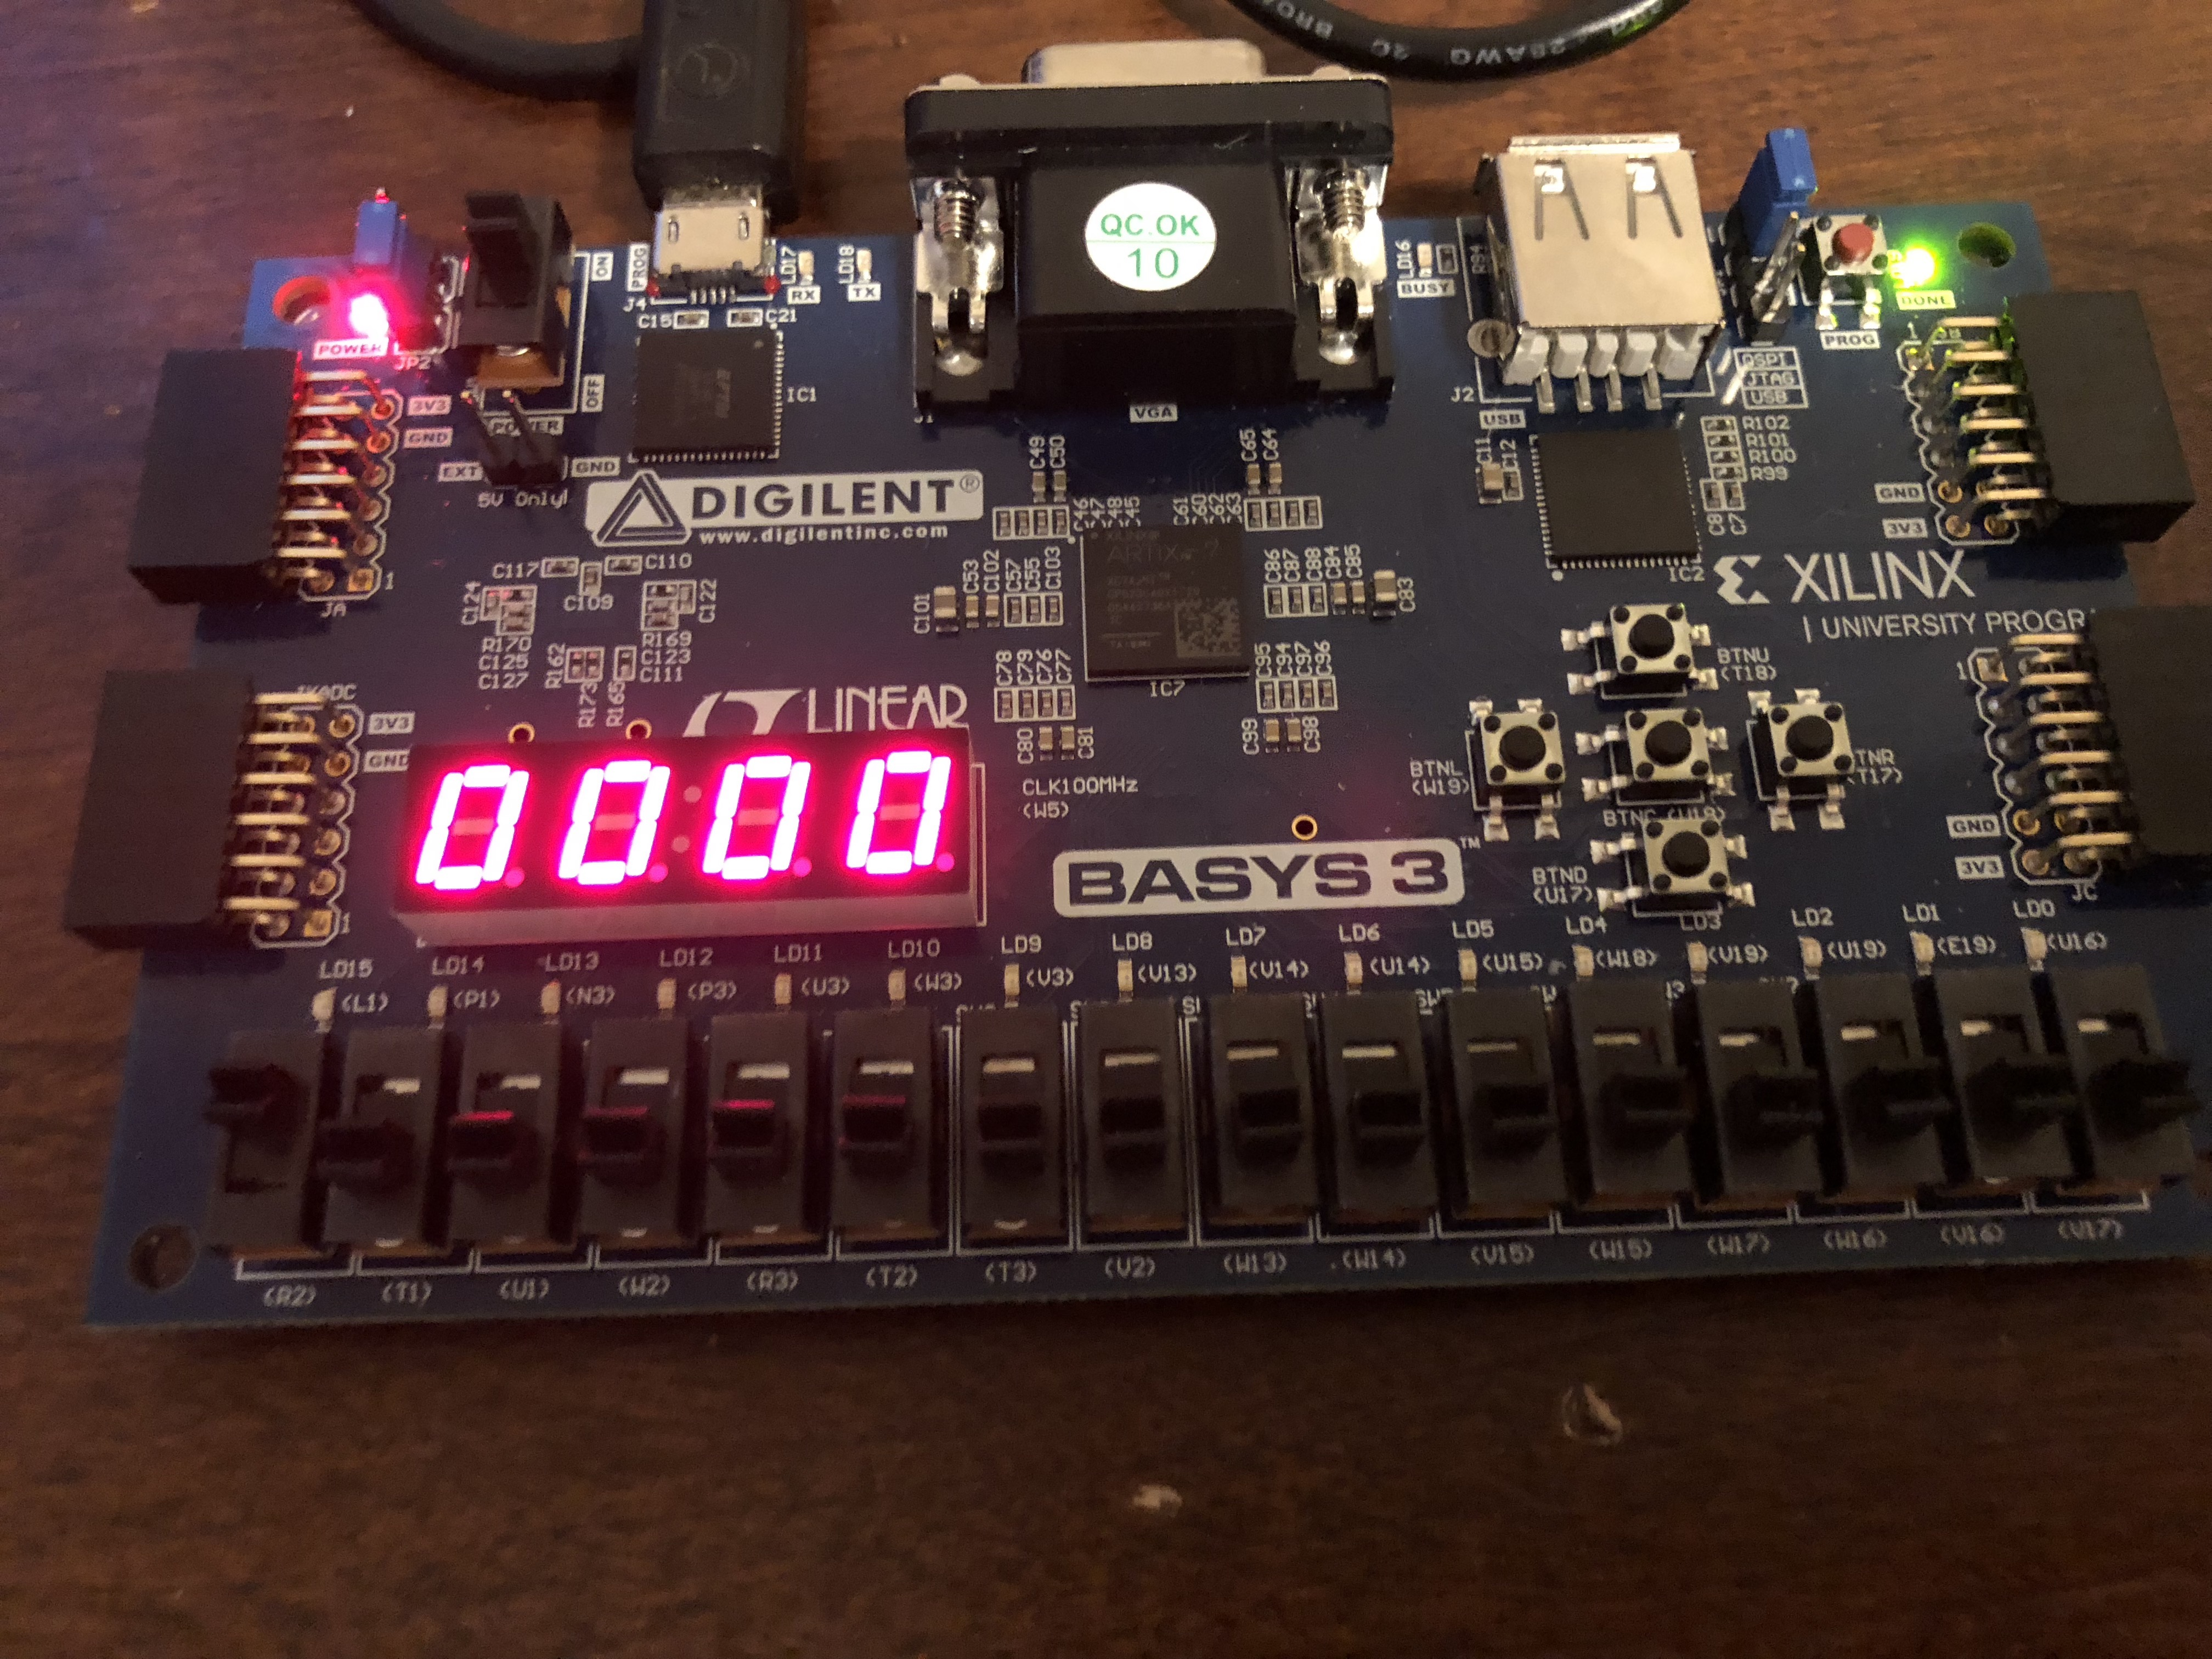
\includegraphics[width=0.5\textwidth]{./images/p3/IMG_1014.jpg}
	\caption{\label{fig:int_res1}Finite state machine has not detected a sequence, counting up.}
\end{center}
\end{figure}

\begin{figure}[H]
\begin{center}
	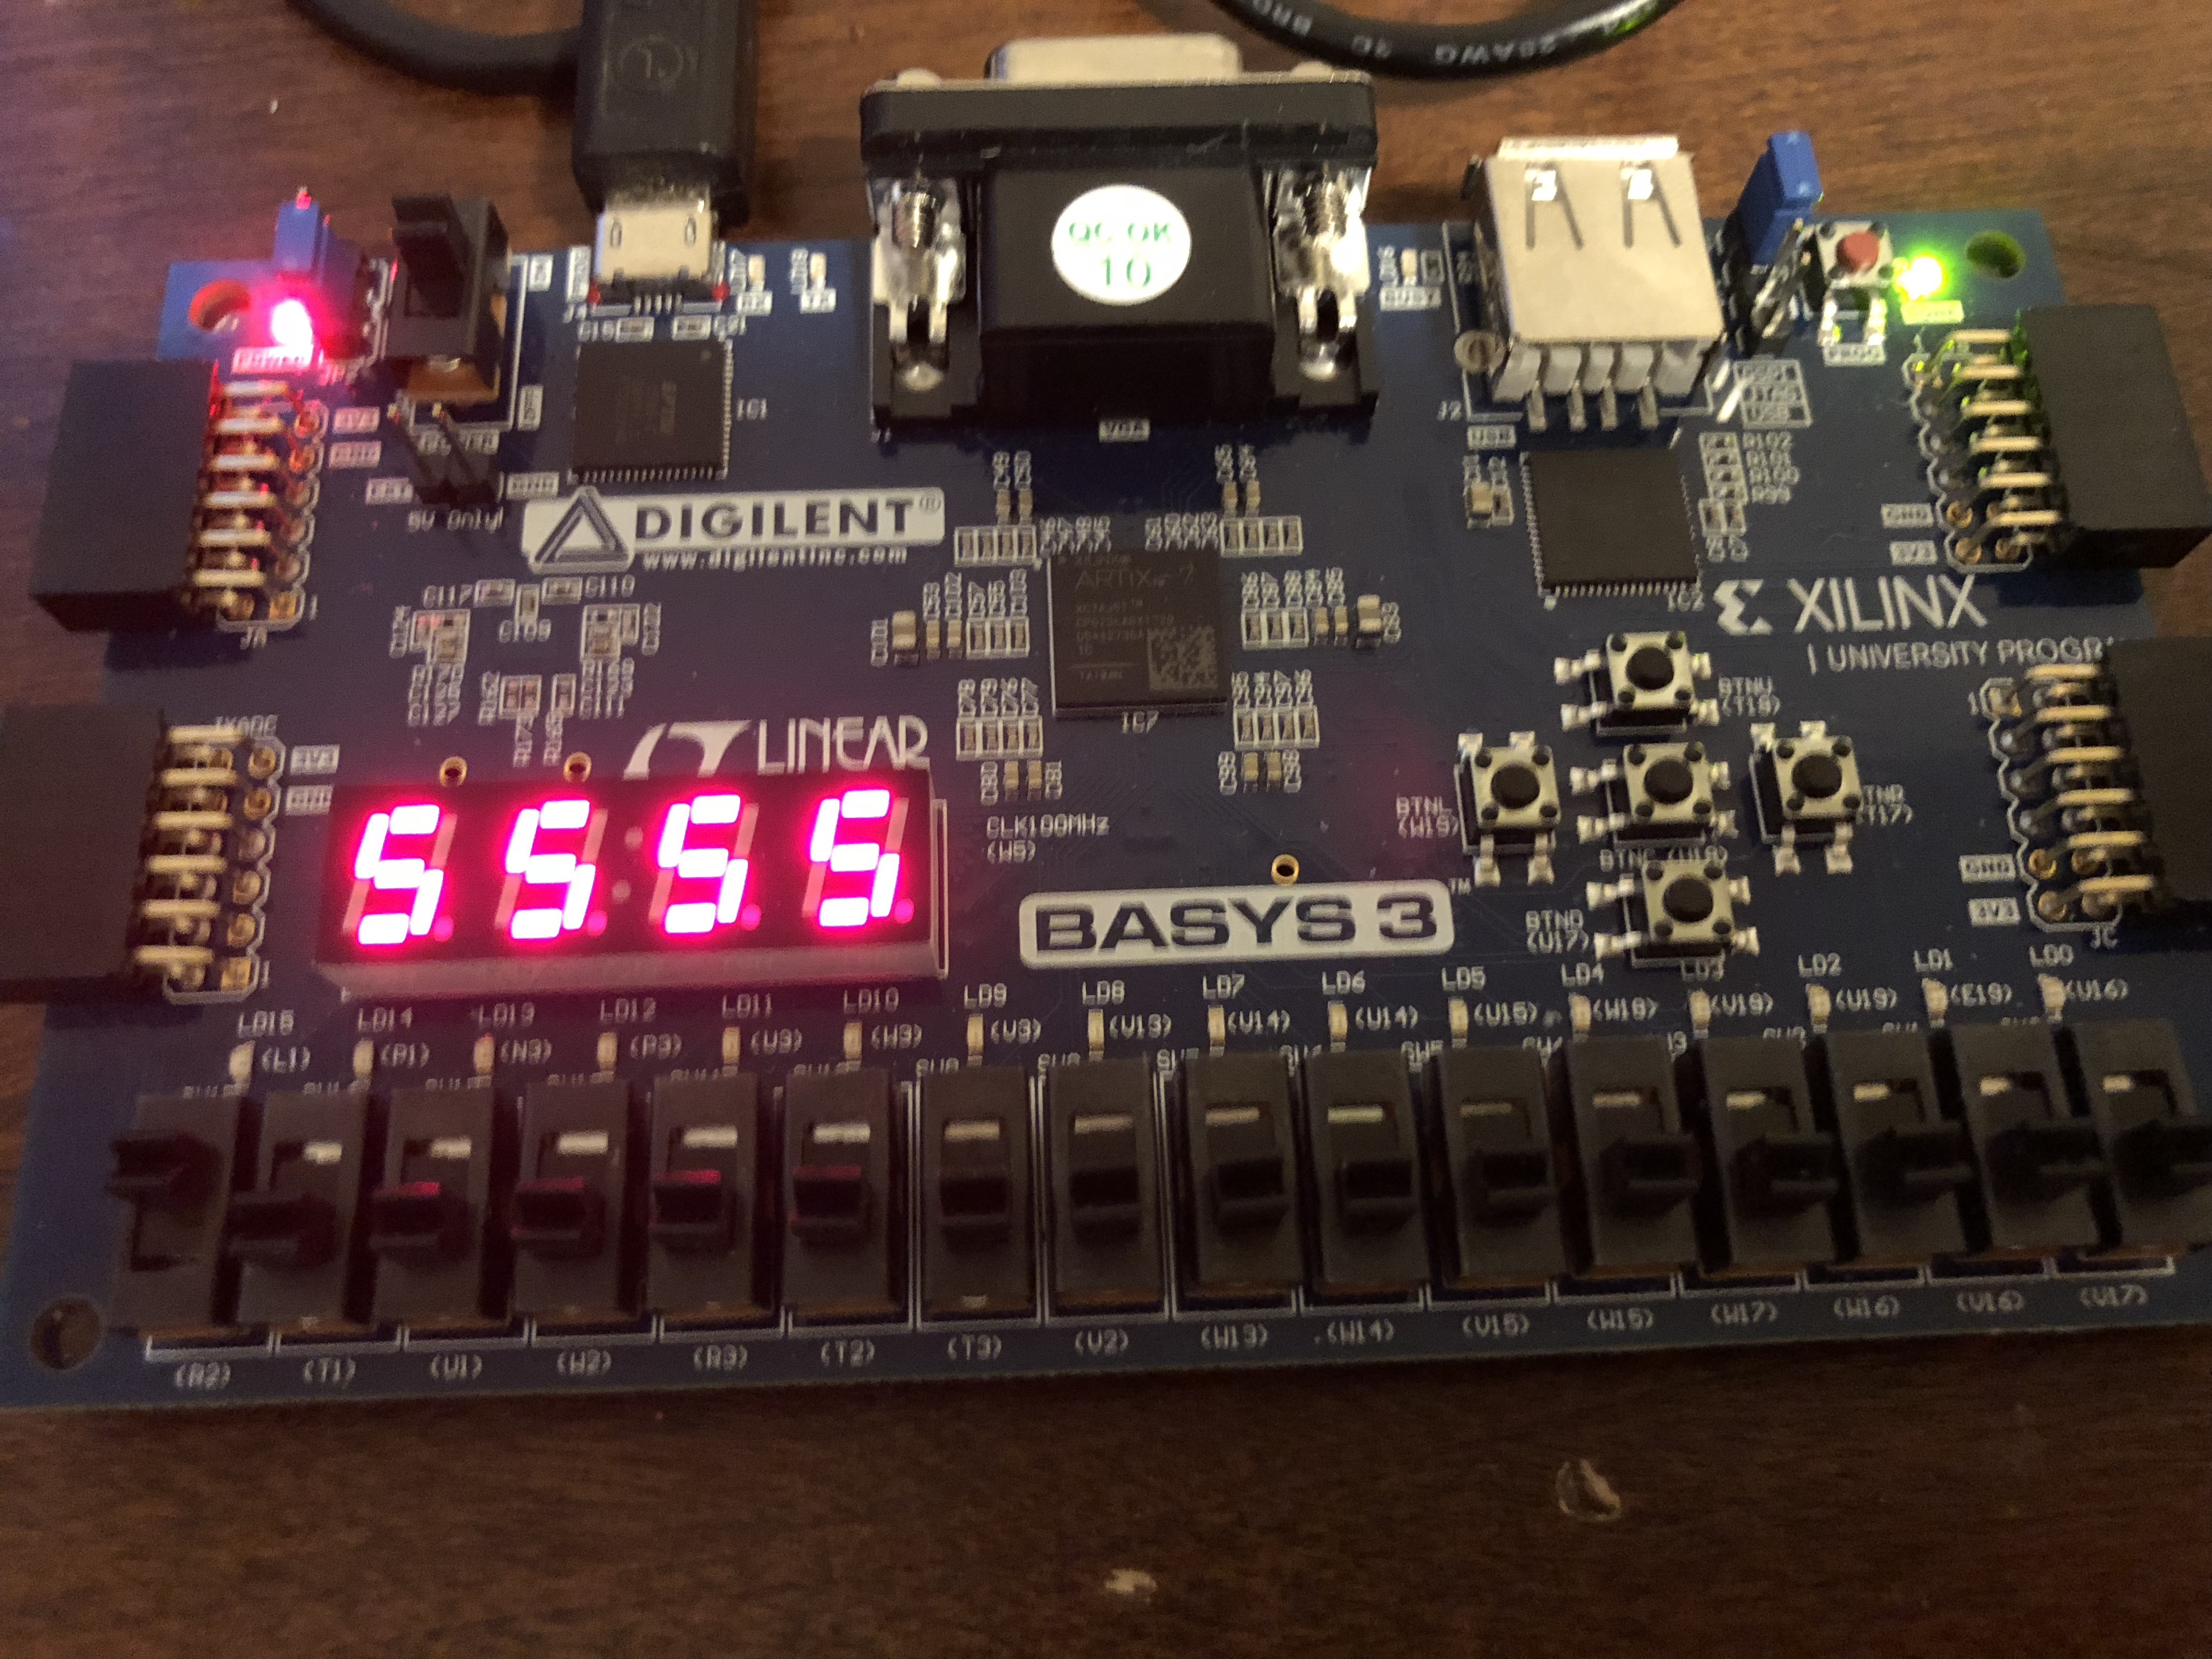
\includegraphics[width=0.5\textwidth]{./images/p3/IMG_1015.jpg}
	\caption{\label{fig:int_res2}Finite state machine has not detected a sequence, counting up.}
\end{center}
\end{figure}

\begin{figure}[H]
\begin{center}
	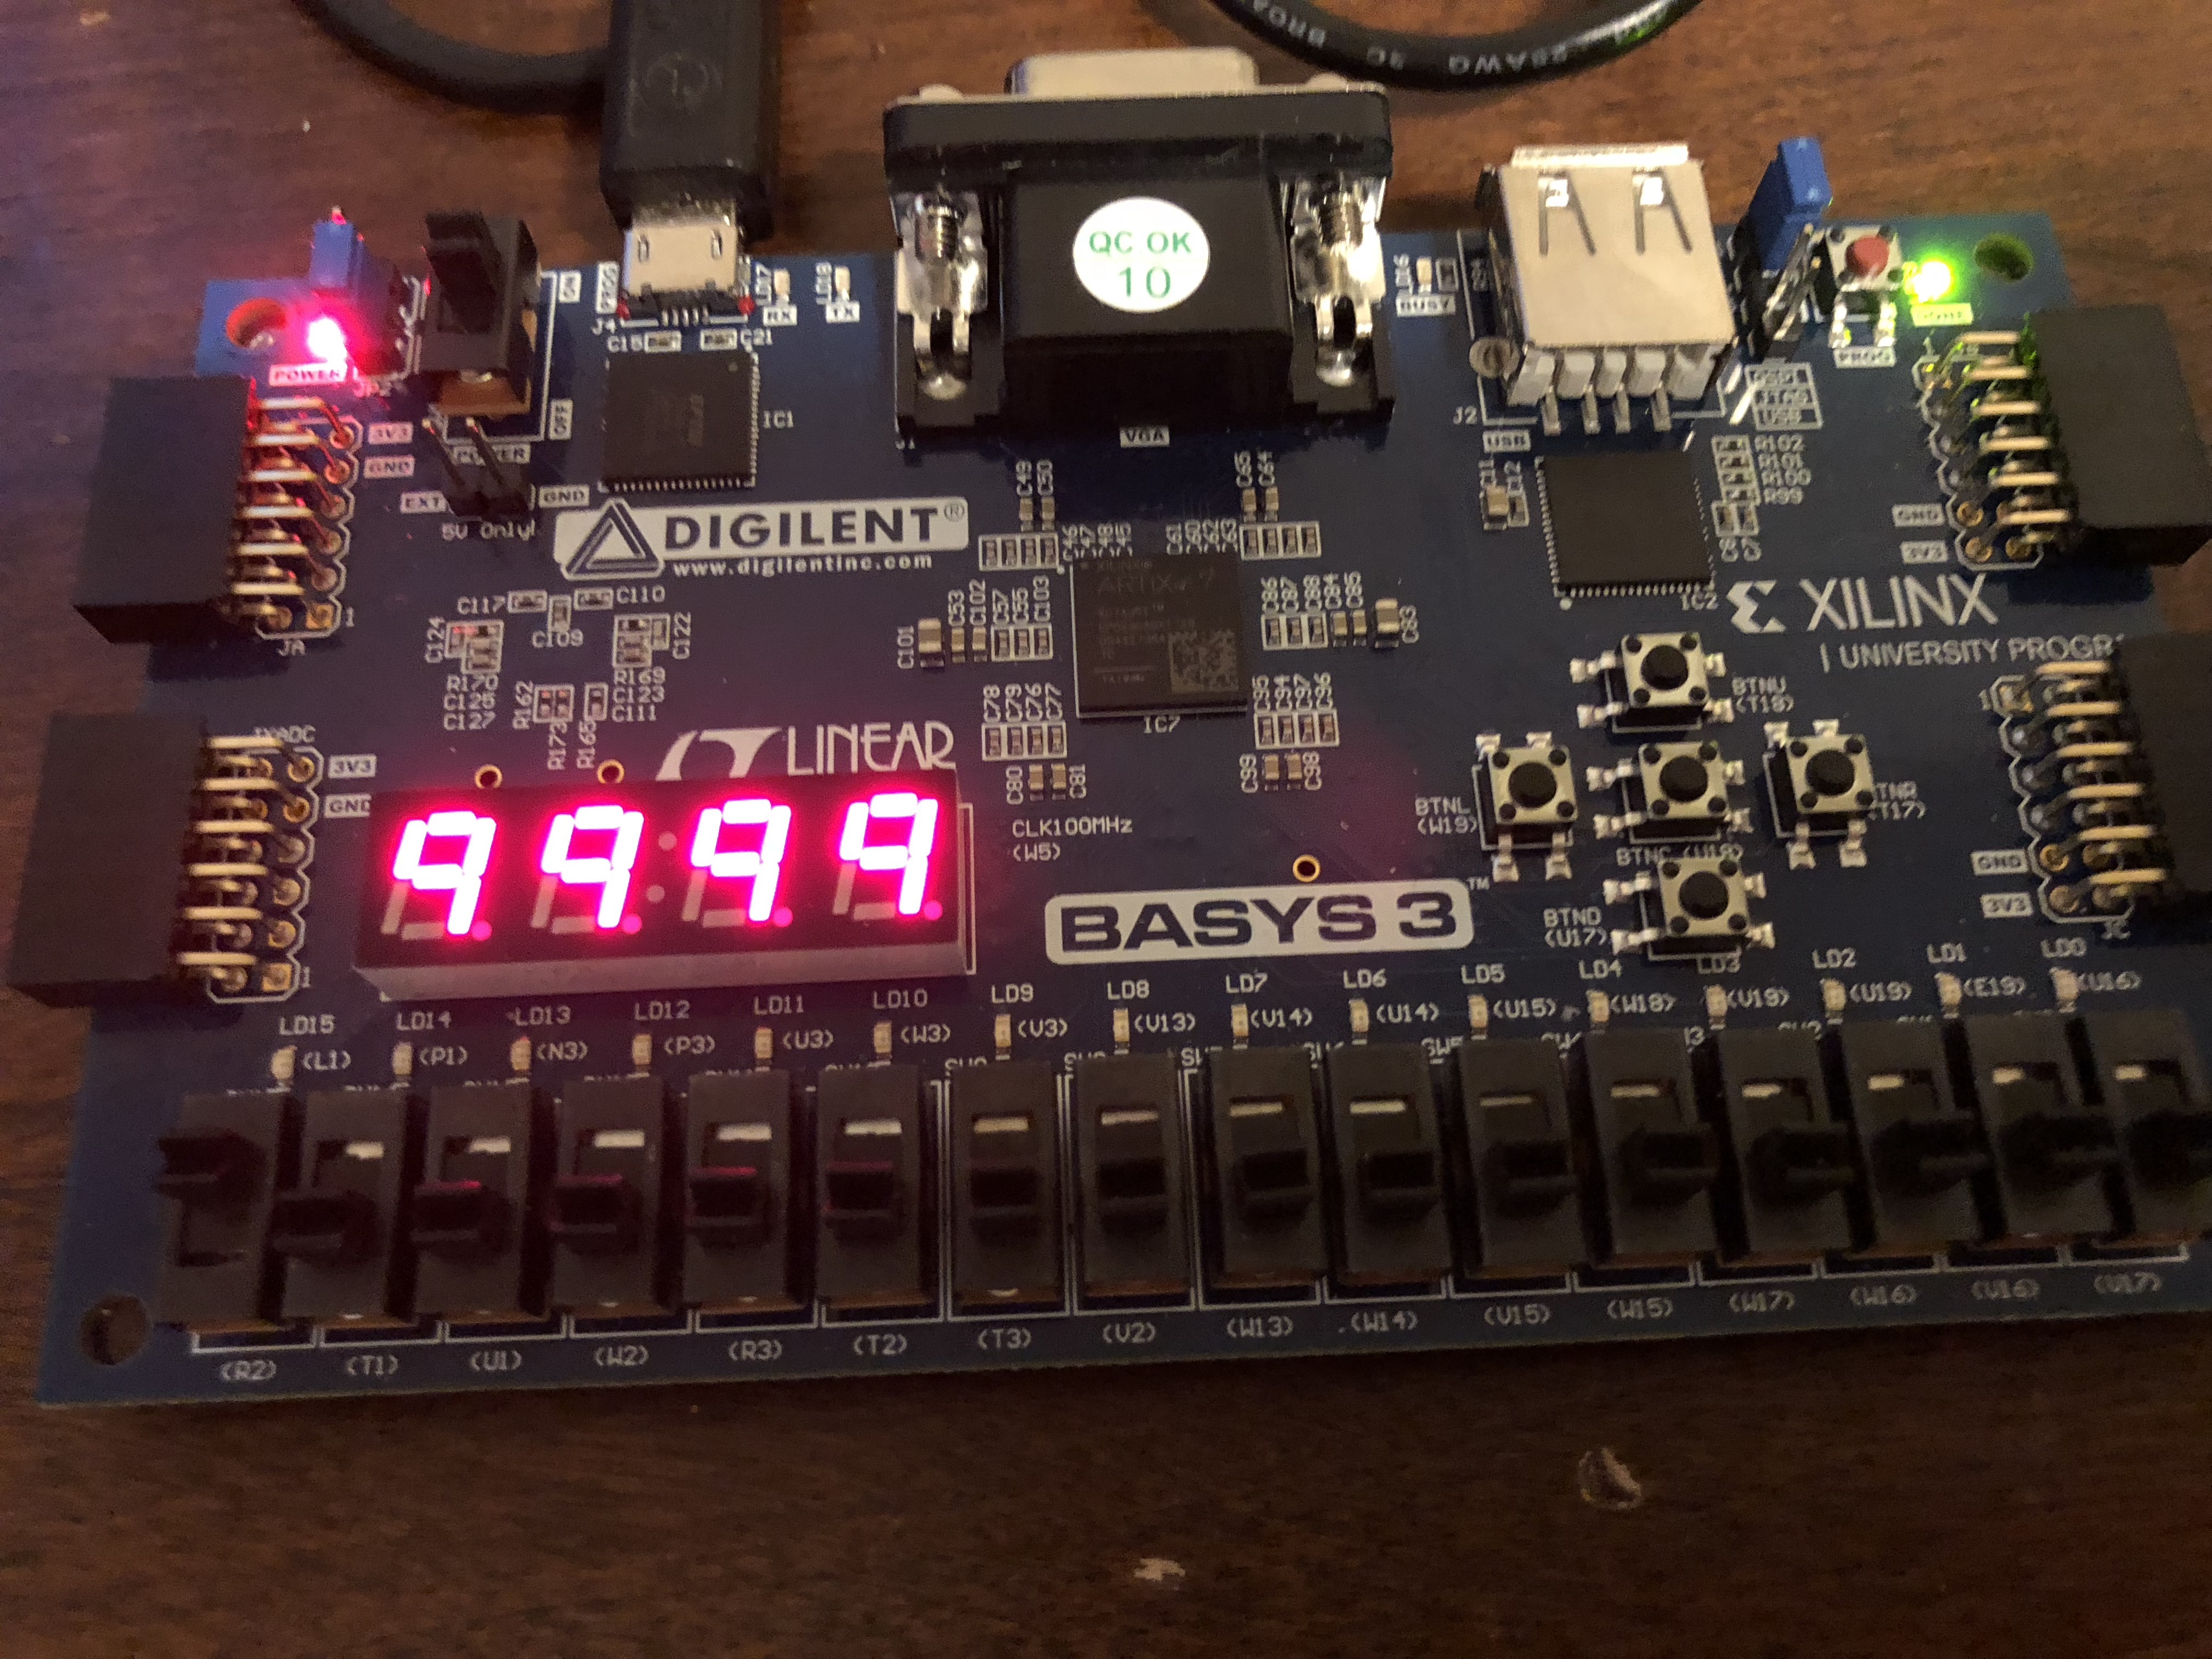
\includegraphics[width=0.5\textwidth]{./images/p3/IMG_1016.jpg}
	\caption{\label{fig:int_res3}Finite state machine has not detected a sequence, counting up.}
\end{center}
\end{figure}

\begin{figure}[H]
\begin{center}
	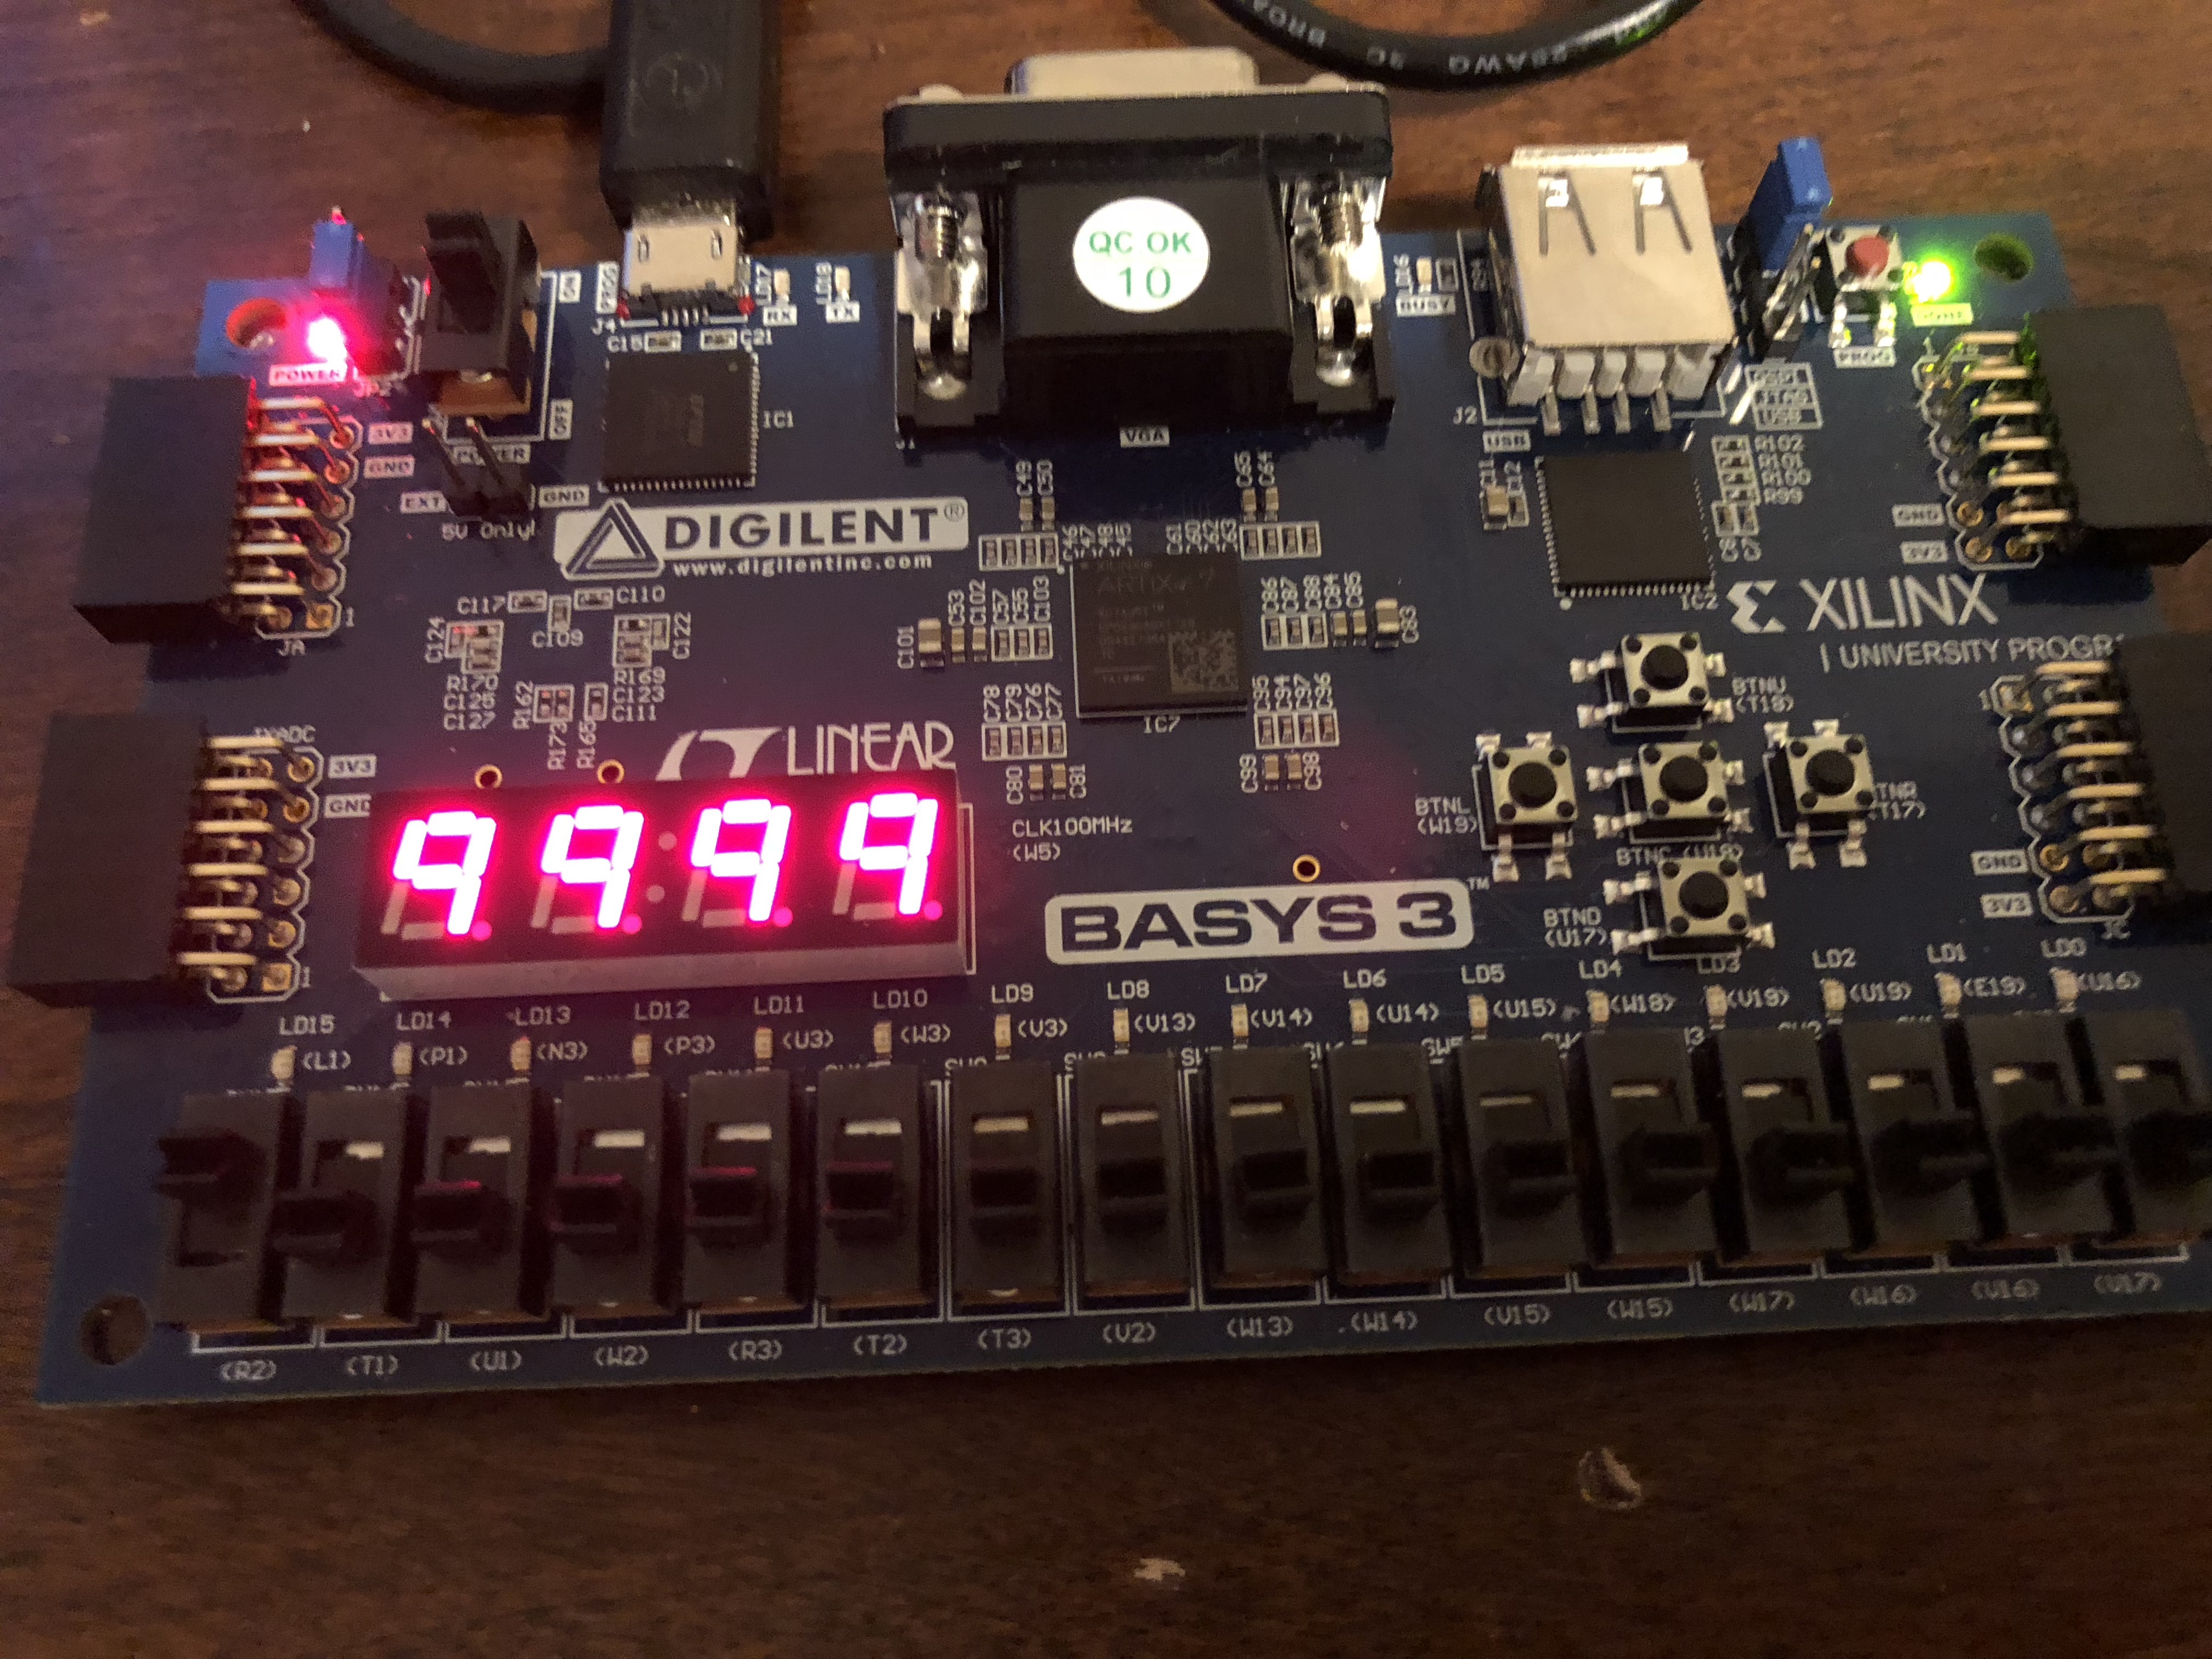
\includegraphics[width=0.5\textwidth]{./images/p3/IMG_1016.jpg}
	\caption{\label{fig:int_res4}Finite state machine has a sequence "010, counting down.}
\end{center}
\end{figure}

\begin{figure}[H]
\begin{center}
	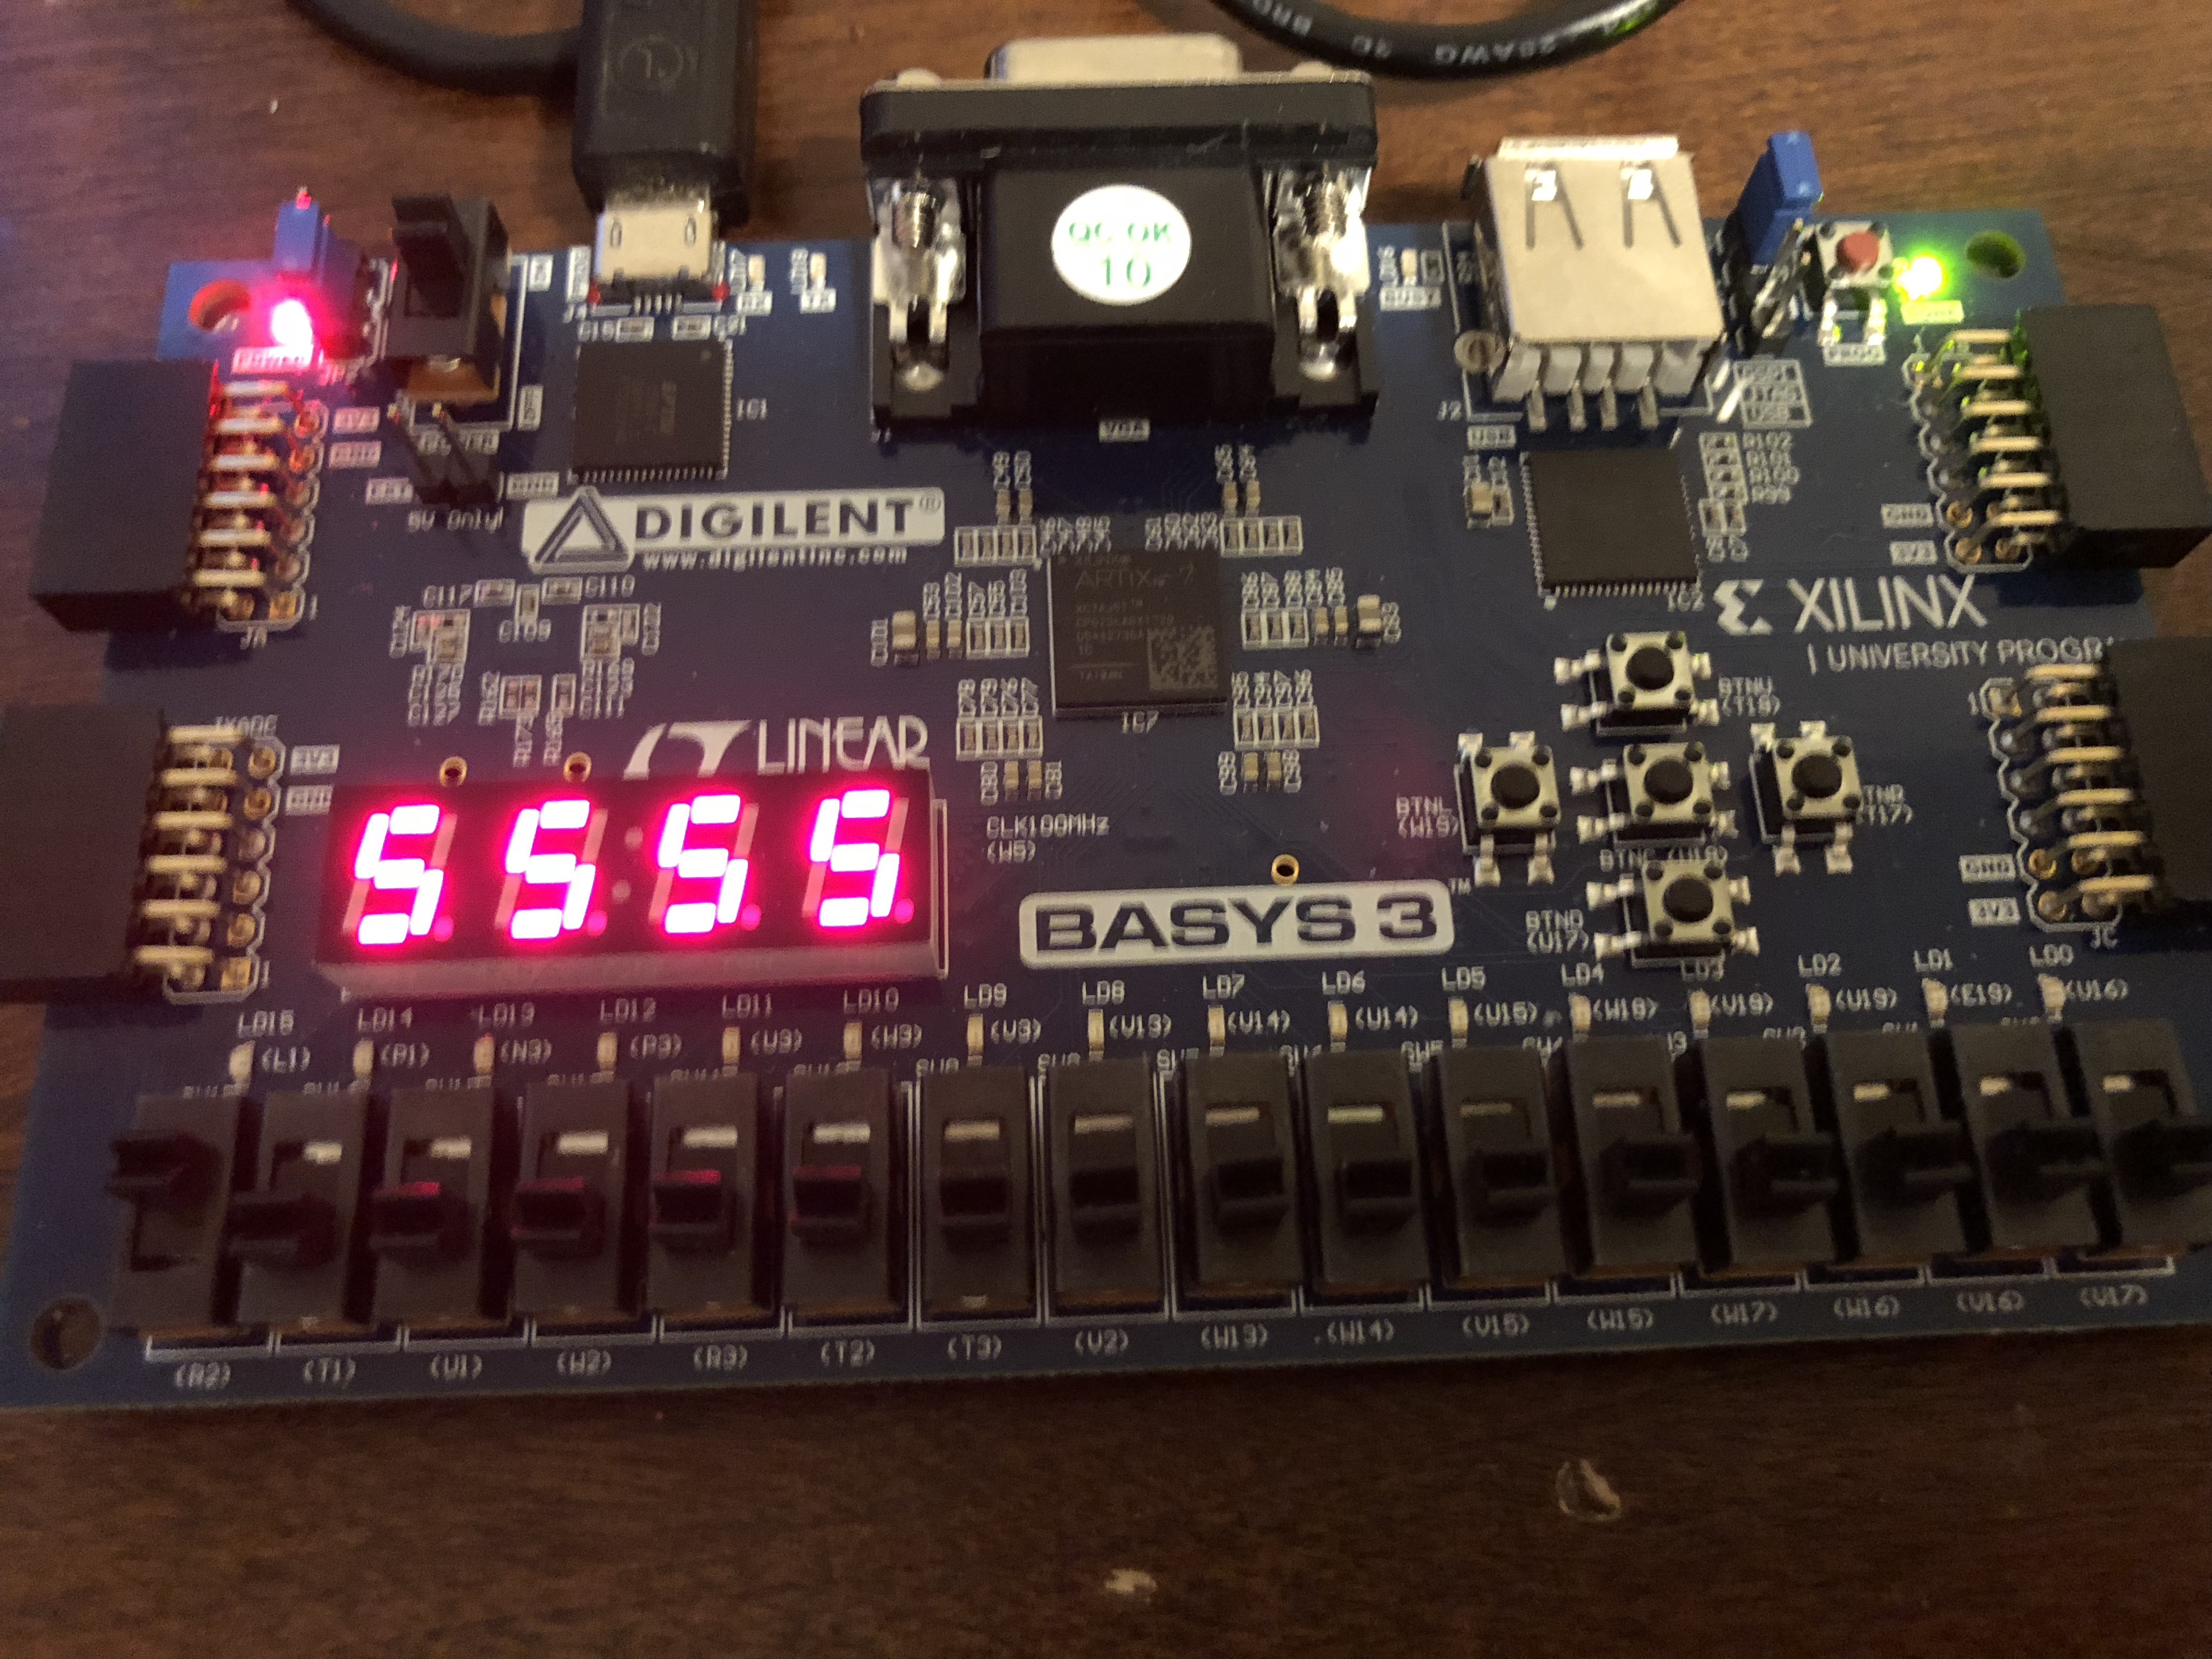
\includegraphics[width=0.5\textwidth]{./images/p3/IMG_1015.jpg}
	\caption{\label{fig:int_res5}Finite state machine has a sequence "010, counting down.}
\end{center}
\end{figure}

\begin{figure}[H]
\begin{center}
	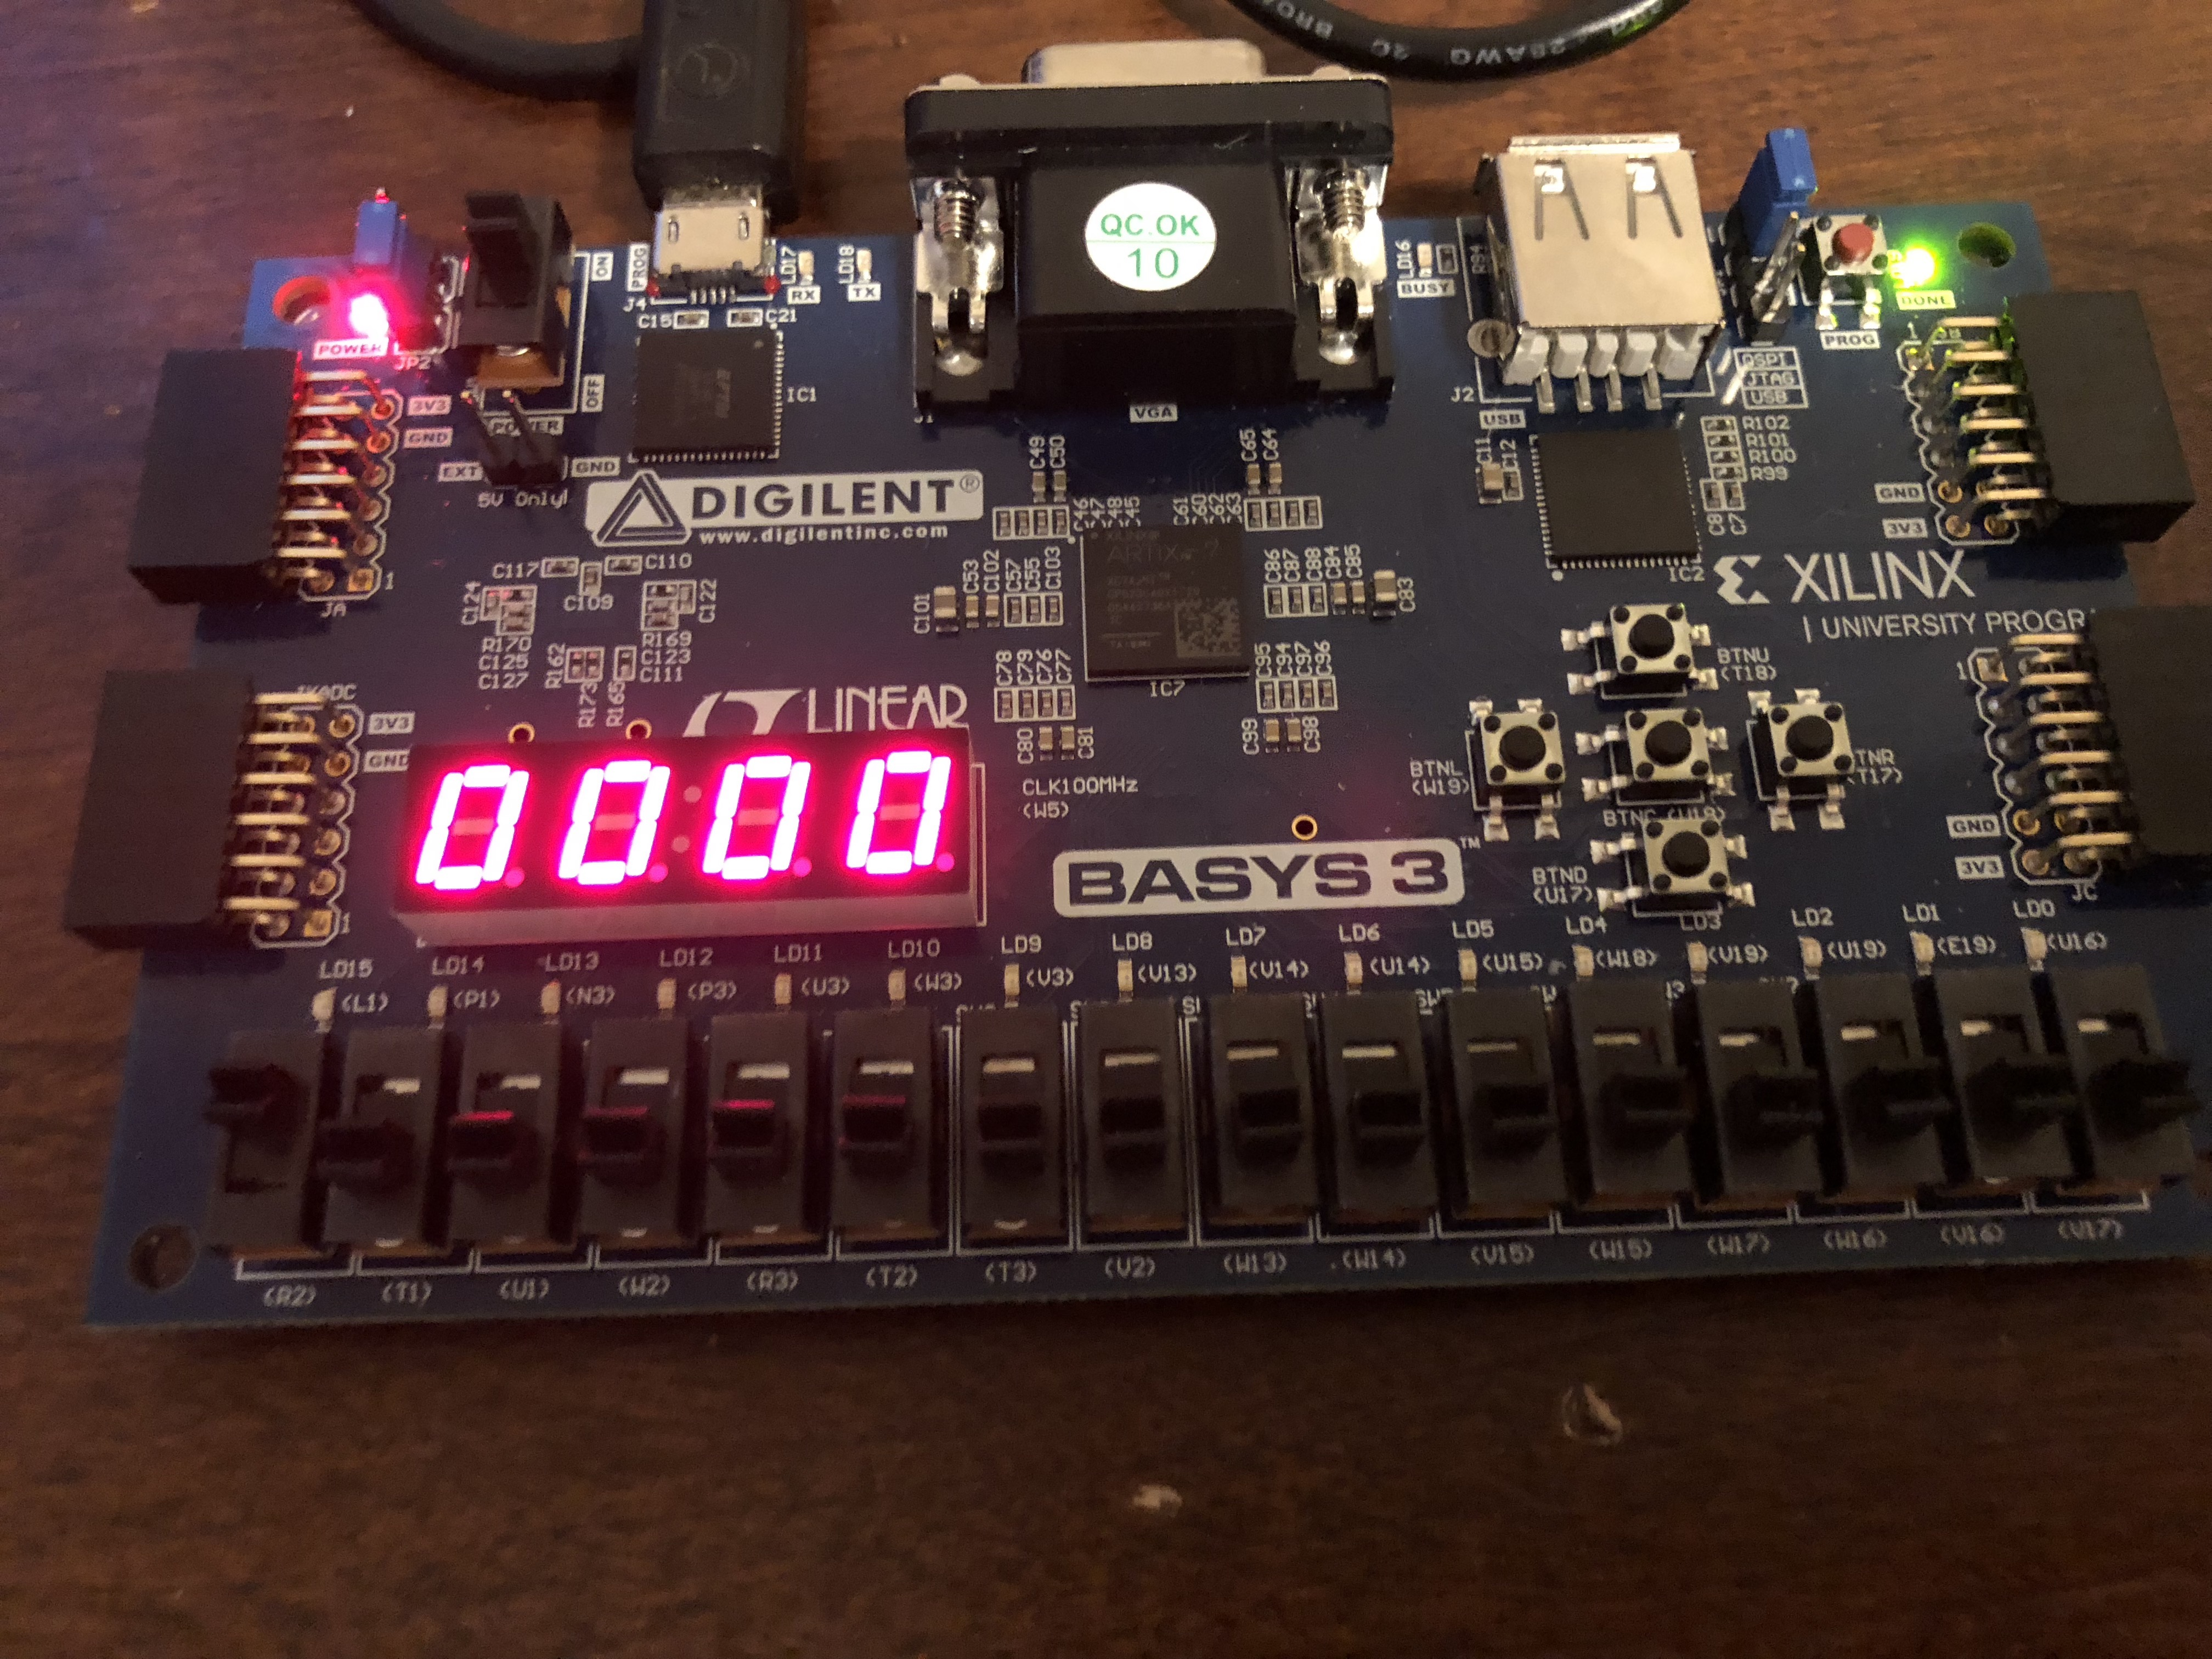
\includegraphics[width=0.5\textwidth]{./images/p3/IMG_1014.jpg}
	\caption{\label{fig:int_res6}Finite state machine has a sequence "010, counting down.}
\end{center}
\end{figure}

\section{Conclusion}
This lab combined two units that we hadn't previously integrated, and it was interesting to watch the counter become increasingly more complex. The most difficult technical challenge was to design a state diagram that would change the direction only when a sequence was detected. Several of our previous iterations would continuously change the counter back to counting down and we had to make adjustments to count correctly.

\pagebreak

\textbf{Appendices}

\begin{appendices}

\section{Problem 1 VHDL Code}

\begin{lstlisting}[language=VHDL]
library IEEE;
use IEEE.STD_LOGIC_1164.ALL;
use IEEE.NUMERIC_STD.ALL;

entity Clockdivider is
     port(clk : in std_logic;
          start_timer : in std_logic;
	  FastClock,MediumClock,SlowClock, led0 : out std_logic);
end Clockdivider;

architecture clockdivider_arch of Clockdivider is

signal slowClock_sig : STD_LOGIC;

begin
    process  
    variable cnt :	
    		std_logic_vector(26 downto 0):= "000000000000000000000000000";
    begin					 
        wait until ((clk'EVENT) AND (clk = '1'));
	       
		if (start_timer = '1') then
	       cnt := "000000000000000000000000000";
	    else  
           cnt := STD_LOGIC_VECTOR(unsigned(cnt) + 1);
	    end if;

   	    FastClock <= cnt(22);
   	    MediumClock <= cnt(24);	
   	    SlowClock <= cnt(26);
        slowClock_sig <= cnt(26);
	
        if (slowClock_sig = '1') then
		  led0 <= '1';
	    else
		  led0 <= '0';
	    end if;
	end process;
end clockdivider_arch;


library IEEE;
use IEEE.STD_LOGIC_1164.ALL;

entity counter is
    Port ( direction : in STD_LOGIC;
           reset : in STD_LOGIC;
           clk : in STD_LOGIC;
           clk_led : out STD_LOGIC;
           count : out STD_LOGIC_VECTOR(6 downto 0));
end counter;

architecture Behavioral of counter is

component Clockdivider is
     port(clk : in std_logic;
          start_timer : in std_logic;
	  FastClock,MediumClock,SlowClock, led0 : out std_logic);
end component Clockdivider;

signal fastClock : STD_LOGIC;
signal mediumClock : STD_LOGIC;
signal slowClock : STD_LOGIC;
signal start_timer : STD_LOGIC := '0';
signal tmp_count : STD_LOGIC_VECTOR(3 downto 0) := "0000";

begin
    clock_div : Clockdivider port map(clk, start_timer, fastClock, 
    		mediumClock, slowClock, clk_led);

    process(clk, reset)
    begin
        if(reset = '1') then tmp_count <= "0000";
        elsif(slowClock'event and (slowClock = '1')) then
            if(direction = '1') then
                case tmp_count is
                    when "0000" =>
                        tmp_count <= "0001";
                    when "0001" =>
                        tmp_count <= "0010";
                    when "0010" =>
                        tmp_count <= "0011";
                    when "0011" =>
                        tmp_count <= "0100";
                    when "0100" =>
                        tmp_count <= "0101";
                    when "0101" =>
                        tmp_count <= "0110";
                    when "0110" =>
                        tmp_count <= "0111";
                    when "0111" =>
                        tmp_count <= "1000";
                    when "1000" =>
                        tmp_count <= "1001";
                    when others =>
                        tmp_count <= "0000";
                end case;
            else
                case tmp_count is
                    when "1001" =>
                        tmp_count <= "1000";
                    when "1000" =>
                        tmp_count <= "0111";
                    when "0111" =>
                        tmp_count <= "0110";
                    when "0110" =>
                        tmp_count <= "0101";
                    when "0101" =>
                        tmp_count <= "0100";
                    when "0100" =>
                        tmp_count <= "0011";
                    when "0011" =>
                        tmp_count <= "0010";
                    when "0010" =>
                        tmp_count <= "0001";
                    when "0001" =>
                        tmp_count <= "0000";
                    when others =>
                        tmp_count <= "1001";
                end case;
            end if;
        end if;
    end process;
    process(tmp_count)
    begin
        case tmp_count is
            when "0000" =>
                count <= "0000001";
            when "0001" =>
                count <= "1001111";
            when "0010" =>
                count <= "0010010";
            when "0011" =>
                count <= "0000110";
            when "0100" =>
                count <= "1001100";
            when "0101" =>
                count <= "0100100";
            when "0110" =>
                count <= "0100000";
            when "0111" =>
                count <= "0001111";
            when "1000" =>
                count <= "0000000";
            when "1001" =>
                count <= "0001100";
            when others =>
                count <= "1111111";
        end case;
    end process;    
    
end Behavioral;
\end{lstlisting}

\section{Problem 1 Constraints File}
\begin{center}
\begin{figure}[H]
	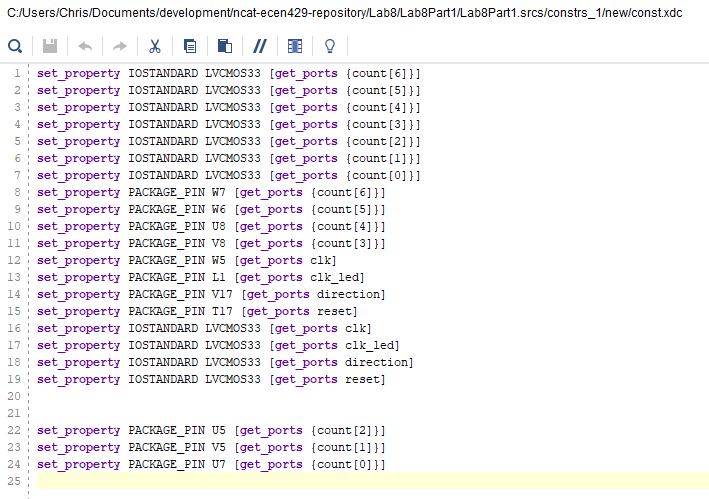
\includegraphics[scale=1]{./images/const1.png}
	\caption{\label{fig:Prob1Const}Constraints file for Problem 1.}
\end{figure}
\end{center}

\section{Problem 2 VHDL Code}
\begin{lstlisting}[language=VHDL]
--Uses ClockDivider from Problem 1.

library IEEE;
use IEEE.STD_LOGIC_1164.ALL;

entity counter is
    Port ( direction : in STD_LOGIC;
           reset : in STD_LOGIC;
           load : in STD_LOGIC;
           enable : in STD_LOGIC;
           clk : in STD_LOGIC;
           input : in STD_LOGIC_VECTOR(3 downto 0);
           clk_led : out STD_LOGIC;
           count : out STD_LOGIC_VECTOR(6 downto 0));
end counter;

architecture Behavioral of counter is

component Clockdivider is
     port(clk : in std_logic;
          start_timer : in std_logic;
	  FastClock,MediumClock,SlowClock, led0 : out std_logic);
end component Clockdivider;

signal fastClock : STD_LOGIC;
signal mediumClock : STD_LOGIC;
signal slowClock : STD_LOGIC;
signal start_timer : STD_LOGIC := '0';
signal tmp_count : STD_LOGIC_VECTOR(3 downto 0) := "0000";

begin
    clock_div : Clockdivider port map(clk, start_timer, fastClock, 
    		mediumClock, slowClock, clk_led);

    process(clk, reset)
    begin
        if(reset = '1') then tmp_count <= "0000";
        elsif(slowClock'event and (slowClock = '1') and enable = '1') then
            if(load = '1') then
                tmp_count <= input;
            elsif(direction = '1') then
                case tmp_count is
                    when "0000" =>
                        tmp_count <= "0001";
                    when "0001" =>
                        tmp_count <= "0010";
                    when "0010" =>
                        tmp_count <= "0011";
                    when "0011" =>
                        tmp_count <= "0100";
                    when "0100" =>
                        tmp_count <= "0101";
                    when "0101" =>
                        tmp_count <= "0110";
                    when "0110" =>
                        tmp_count <= "0111";
                    when "0111" =>
                        tmp_count <= "1000";
                    when "1000" =>
                        tmp_count <= "1001";
                    when others =>
                        tmp_count <= "0000";
                end case;
            else
                case tmp_count is
                    when "1001" =>
                        tmp_count <= "1000";
                    when "1000" =>
                        tmp_count <= "0111";
                    when "0111" =>
                        tmp_count <= "0110";
                    when "0110" =>
                        tmp_count <= "0101";
                    when "0101" =>
                        tmp_count <= "0100";
                    when "0100" =>
                        tmp_count <= "0011";
                    when "0011" =>
                        tmp_count <= "0010";
                    when "0010" =>
                        tmp_count <= "0001";
                    when "0001" =>
                        tmp_count <= "0000";
                    when others =>
                        tmp_count <= "1001";
                end case;
            end if;
        end if;
    end process;
    process(tmp_count)
    begin
        case tmp_count is
            when "0000" =>
                count <= "0000001";
            when "0001" =>
                count <= "1001111";
            when "0010" =>
                count <= "0010010";
            when "0011" =>
                count <= "0000110";
            when "0100" =>
                count <= "1001100";
            when "0101" =>
                count <= "0100100";
            when "0110" =>
                count <= "0100000";
            when "0111" =>
                count <= "0001111";
            when "1000" =>
                count <= "0000000";
            when "1001" =>
                count <= "0001100";
            when others =>
                count <= "1111111";
        end case;
    end process;    
    
end Behavioral;
\end{lstlisting}

\section{Problem 2 Constraints File}
\begin{center}
\begin{figure}[H]
	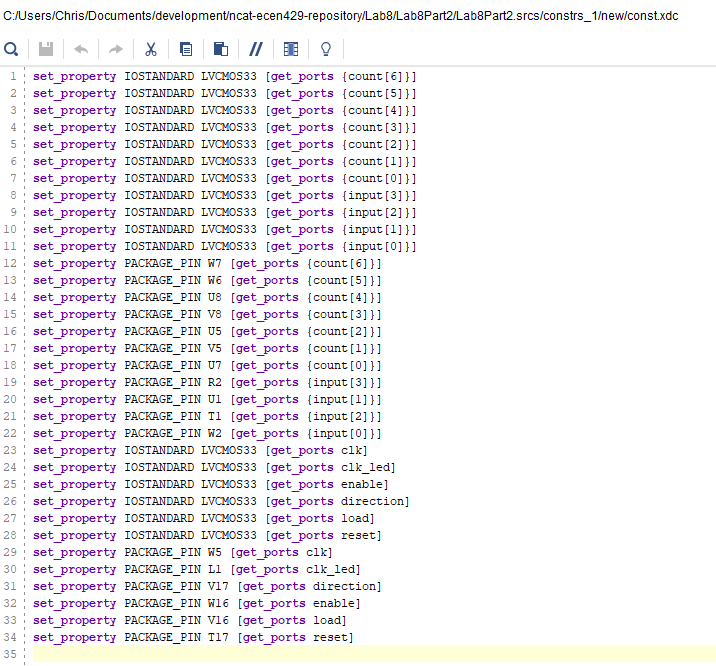
\includegraphics[scale=1]{./images/const2.png}
	\caption{\label{fig:Prob2Const}Constraints file for Problem 2.}
\end{figure}
\end{center}

\section{Problem 3 VHDL Code}
\begin{lstlisting}[language=VHDL]
-- Using Counter from Problem 2.

library IEEE;
use IEEE.STD_LOGIC_1164.ALL;

-- Uncomment the following library declaration if using
-- arithmetic functions with Signed or Unsigned values
--use IEEE.NUMERIC_STD.ALL;

-- Uncomment the following library declaration if instantiating
-- any Xilinx leaf cells in this code.
--library UNISIM;
--use UNISIM.VComponents.all;

entity fsm_control is
    Port ( reset : in STD_LOGIC;
           clk : in STD_LOGIC;
           load : in STD_LOGIC;
           enable : in STD_LOGIC;
           state_input : in STD_LOGIC;
           load_input : in STD_LOGIC_VECTOR(3 downto 0);
           output : out STD_LOGIC_VECTOR(6 downto 0));
end fsm_control;

architecture Behavioral of fsm_control is

component counter is
    Port ( direction : in STD_LOGIC;
           reset : in STD_LOGIC;
           load : in STD_LOGIC;
           enable : in STD_LOGIC;
           clk : in STD_LOGIC;
           input : in STD_LOGIC_VECTOR(3 downto 0);
           clk_led : out STD_LOGIC;
           count : out STD_LOGIC_VECTOR(6 downto 0));
end component counter;

signal state : STD_LOGIC_VECTOR(2 downto 0);
signal slowClock : STD_LOGIC;
signal count : STD_LOGIC_VECTOR(6 downto 0) := "0000000";
signal direction : STD_LOGIC;

begin
    counter_comp : counter port map(direction, reset, load, 
    		enable, clk, load_input, slowClock, count);
    
    process(slowClock, reset, state)
    begin
        if(reset = '1') then
            state <= "000";
        elsif(slowClock'event and slowClock = '1') then
            case state is
                when "000" =>
                    if(state_input = '1') then
                        state <= "001";
                    else
                        state <= "100";
                    end if;
                when "001" =>
                    if(state_input = '1') then
                        state <= "001";
                    else
                        state <= "010";
                    end if;
                when "010" =>
                    if(state_input = '1') then
                        state <= "011";
                        direction <= '1';
                    else
                        state <= "100";
                    end if;
                when "011" =>
                    state <= "000";
                when "100" =>
                    if(state_input = '1') then
                        state <= "101";
                    else
                        state <= "100";
                    end if;
                when "101" =>
                    if(state_input = '1') then
                        state <= "001";
                    else
                        state <= "110";
                        direction <= '0';
                    end if;
                when others =>
                    state <= "000";
            end case;
        end if;
    end process; 


    output <= count;

end Behavioral;
\end{lstlisting}

\section{Problem 3 Constraints File}
\begin{center}
\begin{figure}[H]
	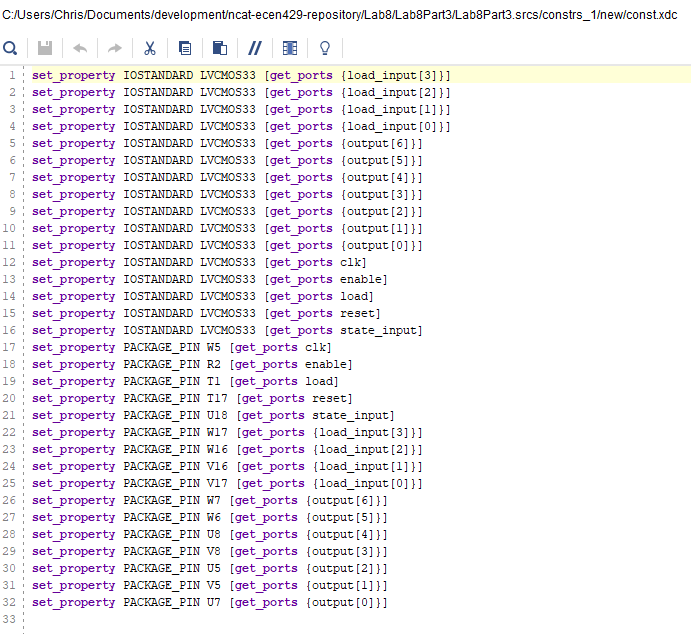
\includegraphics[scale=1]{./images/const3.png}
	\caption{\label{fig:Prob3Const}Constraints file for Problem 3.}
\end{figure}
\end{center}

\end{appendices}
\end{document}
